%!TEX encoding = UTF-8 Unicode
\documentclass[10pt,a4paper]{article}
\usepackage[T1]{fontenc}
\usepackage[utf8]{inputenc}
\usepackage{fourier}
\usepackage[scaled=0.875]{helvet}
\renewcommand{\ttdefault}{lmtt}
\usepackage{makeidx}
\makeindex
\usepackage{amsmath,amssymb}
\usepackage{fancybox}
\usepackage[normalem]{ulem}
\usepackage{pifont}
\usepackage{lscape}
\usepackage{multicol}
\usepackage{mathrsfs}
\usepackage{tabularx,array}
\usepackage{colortbl}
\usepackage{multirow}
\usepackage{textcomp}
\usepackage{enumitem}  
\newcommand{\euro}{\eurologo{}}
%Tapuscrit : Denis Vergès 
\usepackage{graphicx}
\usepackage{pst-plot,pst-tree,pstricks,pst-node,pst-func,pstricks-add}
\usepackage{pst-eucl}
\usepackage{pstricks-add}
\newcommand{\R}{\mathbb{R}}
\newcommand{\N}{\mathbb{N}}
\newcommand{\D}{\mathbb{D}}
\newcommand{\Z}{\mathbb{Z}}
\newcommand{\Q}{\mathbb{Q}}
\newcommand{\C}{\mathbb{C}}
\usepackage{diagbox}
\usepackage[left=3.5cm, right=3.5cm, top=2cm, bottom=3cm]{geometry}
\def\e{\text{e}}
\def\i{\text{i}}
\newcommand{\ds}{\displaystyle}%   displaystyle
\newcommand{\cg}{\texttt{]}}% crochet gauche
\newcommand{\cd}{\texttt{[}}% crochet droit
\newcommand{\pg}{\geqslant}%  plus grand ou égal
\newcommand{\pp}{\leqslant}%  plus petit ou égal
\newcommand{\vect}[1]{\overrightarrow{\,\mathstrut#1\,}}
\newcommand{\barre}[1]{\overline{\,\mathstrut#1\,}}
\renewcommand{\theenumi}{\textbf{\arabic{enumi}}}
\renewcommand{\labelenumi}{\textbf{\theenumi.}}
\renewcommand{\theenumii}{\textbf{\alph{enumii}}}
\renewcommand{\labelenumii}{\textbf{\theenumii.}}
\def\Oij{$\left(\text{O},~\vect{\imath},~\vect{\jmath}\right)$}
\def\Oijk{$\left(\text{O},~\vect{\imath},~\vect{\jmath},~\vect{k}\right)$}
\def\Ouv{$\left(\text{O},~\vect{u},~\vect{v}\right)$}
\usepackage{fancyhdr}
\usepackage[dvips,colorlinks=true,pdfstartview=FitV,linkcolor=blue,citecolor=blue,urlcolor=blue]{hyperref}
\hypersetup{%
pdfauthor = {APMEP},
pdfsubject = {Baccalauréat S},
pdftitle = {Baccalauréat S -  2018},
allbordercolors = white,
pdfstartview=FitH} 
\usepackage[frenchb]{babel}
\usepackage[np]{numprint}
\begin{document}
\setlength\parindent{0mm}
\rhead{\textbf{A. P{}. M. E. P{}.}}
\lhead{\small{Baccalauréat S : l'intégrale 2018}}
\pagestyle{fancy}
\thispagestyle{empty} 
\begin{center}
{\huge\textbf{\decofourleft~Baccalauréat S  
2018~\decofourright\\ \vspace{1cm} L'intégrale de mai à novembre
 2018}}

\vspace{1cm}

Pour un accès direct cliquez sur les liens {\Large 
\textcolor{blue}{bleus}}
\end{center}

\vspace{1cm}
 
\begin{tabularx}{\linewidth}{>{\Large}X} 
\Large \hyperlink{Pondichery}{Pondichéry  4 mai 2018} \dotfill \pageref{Pondichery}\\
\hyperlink{Liban}{Liban  29 mai 2018} \dotfill \pageref{Liban}\\
\hyperlink{AmeriqueNord}{Amérique du Nord 29 mai 2018} \dotfill \pageref{AmeriqueNord}\\
\hyperlink{Centresetrangers}{Centres étrangers 11  juin 2018} \dotfill \pageref{Centresetrangers}\\
\hyperlink{Antilles}{Antilles-Guyane 19 juin 2018} \dotfill \pageref{Antilles}\\
\hyperlink{Polynesie}{Polynésie 20 juin 2018} \dotfill \pageref{Polynesie}\\
\hyperlink{Asie}{Asie 21 juin 2018} \dotfill \pageref{Asie}\\
\hyperlink{Metropole}{Métropole  22 juin 2018} \dotfill \pageref{Metropole}\\
%\hyperlink{Polynesiesep}{Polynésie 5  septembre 2018} \dotfill \pageref{Polynesiesep}\\
\hyperlink{Antillessep}{Antilles-Guyane  6 septembre 2018} \dotfill \pageref{Antillessep}\\
\hyperlink{Metropolesep}{Métropole  12 septembre 2018} \dotfill \pageref{Metropolesep}\\
\hyperlink{AmeriSud}{Amérique du Sud  13 novembre 2018}\dotfill \pageref{AmeriSud}\\
\hyperlink{Caledonienov}{Nouvelle-Calédonie   27 novembre 2018} \dotfill \pageref{Caledonienov}\\
%\hyperlink{Caledoniefevrier}{Nouvelle-Calédonie   5 mars 2018} \dotfill \pageref{Caledoniefevrier}
\end{tabularx}
 
\vspace{1cm}\hyperlink{Index}{À la fin index des notions abordées}

%À la fin de chaque exercice cliquer sur {\blue *} pour aller à l'index
\newpage ~
\newpage
%%%%%%%%%%% Pondichéry 4 mai 2018
\hypertarget{Pondichery}{}

\label{Pondichery}
\lhead{\small Baccalauréat S}
\lfoot{\small{Pondichéry}}
\rfoot{\small{4 mai 2018}}
\pagestyle{fancy}
\thispagestyle{empty}

\begin{center}{\Large\textbf{\decofourleft~Baccalauréat S Pondichéry 4 mai 2018~\decofourright}}
\end{center}

\vspace{0,25cm}

\textbf{\textsc{Exercice 1} \hfill 6 points}
 
\textbf{Commun  à tous les candidats}

\medskip

\emph{Les parties } A \emph{et}   B \emph{peuvent être traitées de façon indépendante.}

\bigskip


Dans une usine, un four cuit des céramiques à la température de \np{1000}~\degres C. À la fin de la
cuisson, il est éteint et il refroidit.

\smallskip

On s'intéresse à la phase de refroidissement du four, qui débute dès l'instant où il est éteint.

\smallskip

La température du four est exprimée en degré Celsius (\degres~C).

\smallskip

La porte du four peut être ouverte sans risque pour les céramiques dès que sa température est
inférieure à $70$~\degres C. Sinon les céramiques peuvent se fissurer, voire se casser.

\bigskip

\textbf{Partie A}

\medskip

Pour un nombre entier naturel $n$, on note $T_n$ la température en degré Celsius du four au bout
de $n$ heures écoulées à partir de l'instant où il a été éteint. On a donc $T_0 = \np{1000}$.

La température $T_n$ est calculée par l'algorithme suivant :\index{algorithme}

\begin{center}
\begin{tabularx}{0.35\linewidth}{|X|}\hline
$T \gets \np{1000}$\\
Pour $i$ allant de $1$ à $n$\\
\hspace{1cm}$T \gets 0,82 \times T + 3,6$\\
Fin Pour\\\hline
\end{tabularx}
\end{center}

\medskip

\begin{enumerate}
\item Déterminer la température du four, arrondie à l'unité, au bout de $4$ heures de
refroidissement.
\item Démontrer que, pour tout nombre entier naturel $n$, on a : $T_n = 980 \times 0,82^n + 20$.
\item Au bout de combien d'heures le four peut-il être ouvert sans risque pour les céramiques ?
 \end{enumerate}
 
\bigskip

\textbf{Partie B}

\medskip

Dans cette partie, on note $t$ le temps (en heure) écoulé depuis l'instant où le four a été éteint.

La température du four (en degré Celsius) à l'instant $t$ est donnée par la fonction $f$ définie,
pour tout nombre réel $t$ positif, par : 

\[f(t) = a\text{e}^{- \frac{t}{5}} + b,\]\index{fonction exponentielle}

où $a$ et $b$ sont deux nombres réels.

On admet que $f$ vérifie la relation suivante : $f'(t) + \dfrac{1}{5}f(t) = 4$.\index{equation différentielle@équation différentielle}
\medskip

\begin{enumerate}
\item Déterminer les valeurs de $a$ et $b$ sachant qu'initialement, la température du four est de
$\np{1000}$~\degres C, c'est-à-dire que $f(0) = \np{1000}$.
\item  Pour la suite, on admet que, pour tout nombre réel positif $t$: 

\[f(t) = 980\text{e}^{- \frac{t}{5}} + 20.\]

\medskip

	\begin{enumerate}
		\item Déterminer la limite de $f$ lorsque $t$ tend vers $+ \infty$.\index{limite de fonction}
		\item Étudier les variations de $f$ sur $[0~;~+ \infty[$. 
		
En déduire son tableau de variations complet.
		\item Avec ce modèle, après combien de minutes le four peut-il être ouvert sans risque pour
 les céramiques ?
 	\end{enumerate}
\item  La température moyenne (en degré Celsius) du four entre deux instants $t_1$ et $t_2$ est donnée
par: $\dfrac{1}{t_2 - t_1}\displaystyle\int_{t_1}^{t_2} f(t)\:\text{d}t$.\index{valeur moyenne}

	\begin{enumerate}
		\item À l'aide de la représentation graphique de $f$ ci-dessous, donner une estimation de la
température moyenne $\theta$ du four sur les $15$ premières heures de refroidissement.\index{lecture graphique}
		
Expliquer votre démarche.
		
\begin{center}
\psset{xunit=0.6cm,yunit=0.01cm}
\begin{pspicture}(-1,-50)(19,1100)
\multido{\n=0+1}{20}{\psline[linestyle=dashed,linewidth=0.5pt](\n,0)(\n,1100)}
\multido{\n=0+100}{11}{\psline[linestyle=dashed,linewidth=0.5pt](0,\n)(19,\n)}
\psaxes[linewidth=1.25pt,Dy=200]{->}(0,0)(0,0)(19,1100)
\psaxes[linewidth=1.25pt,Dy=200](0,0)(0,0)(19,1100)
\uput[d](16.4,-40){temps écoulé (en heure)}
\uput[r](0,1080){température (en \degres C)}
\psplot[plotpoints=3000,linewidth=1.25pt,linecolor=blue]{0}{19}{980 2.71828 0.2 x mul exp div 20 add}
\end{pspicture}
\end{center}
\medskip

		\item  Calculer la valeur exacte de cette température moyenne $\theta$ et en donner la valeur
arrondie au degré Celsius.
	\end{enumerate}
\item  Dans cette question, on s'intéresse à l'abaissement de température (en degré Celsius) du
four au cours d'une heure, soit entre deux instants $t$ et $(t + 1)$. Cet abaissement est donné
par la fonction $d$ définie, pour tout nombre réel $t$ positif, par : $d(t) = f(t) - f(t + 1)$.
	\begin{enumerate}
		\item Vérifier que. pour tout nombre réel $t$ positif: $d(t) = 980\left(1 - \text{e}^{- \frac{1}{5}}\right)\text{e}^{- \frac{t}{5}}$.
		\item Déterminer la limite de $d(t)$ lorsque $t$ tend vers $+ \infty$.
		
Quelle interprétation peut-on en donner ?
 	\end{enumerate}
\end{enumerate}

\newpage

\textbf{\textsc{Exercice 2} \hfill 4 points}
 
\textbf{Commun  à tous les candidats}

\medskip

Le plan est muni d'un repère orthonormé \Ouv.

\smallskip

Les points A, B et C ont pour affixes respectives $a = - 4,\: b = 2$ et $c = 4$.\index{complexes}

\medskip

\begin{enumerate}
\item On considère les trois points A$'$, B$'$ et C$'$ d'affixes respectives $a'= \text{j}a$, $b'= \text{j}b$ et $c'= \text{j}c$ où j est le nombre complexe $-\dfrac{1}{2} + \text{i}\dfrac{\sqrt{3}}{2}$.

	\begin{enumerate}
		\item Donner la forme trigonométrique et la forme exponentielle de j.
		
En déduire les formes algébriques et exponentielles de $a'$, $b'$ et $c'$.
		\item Les points A, B et C ainsi que les cercles de centre O et de rayon 2, 3 et 4 sont
représentés sur le graphique fourni en \textbf{Annexe}.
		
Placer les points A$'$, B$'$ et C$'$ sur ce graphique.
	\end{enumerate}
\item Montrer que les points A$'$, B$'$ et C$'$ sont alignés.
\item On note M le milieu du segment [A$'$C], N le milieu du segment [C$'$C] et P le milieu du
segment [C$'$A]. 
	
Démontrer que le triangle MNP est isocèle.\index{géométrie plane}
\end{enumerate}

\vspace{0,5cm}

\textbf{\textsc{Exercice 3} \hfill 5 points}
 
\textbf{Commun à tous les candidats}

\medskip

Une entreprise conditionne du sucre blanc provenant de deux exploitations U et V en paquets
de 1 kg et de différentes qualités.

\smallskip

Le sucre extra fin est conditionné séparément dans des paquets portant le label \og  extra fin \fg.

\smallskip

\emph{Les parties \rm{A}, \rm{B} et \rm{C} peuvent être traitées de façon indépendante.}

\smallskip

Dans tout l'exercice, les résultats seront arrondis, si nécessaire, au millième.

\bigskip

\textbf{Partie A}

\medskip

Pour calibrer le sucre en fonction de la taille de ses cristaux, on le fait passer au travers d'une
série de trois tamis positionnés les uns au-dessus des autres et posés sur un récipient à fond
étanche.
Les ouvertures des mailles sont les suivantes :

\begin{center}
\psset{unit=1cm}
\begin{pspicture}(12,4)
%\psgrid
\uput[r](0.5,3){Tamis 1 : 0,8 mm} \psline[linewidth=1.5pt]{->}(4.6,1)(6.8,1)
\uput[r](0.5,2){Tamis 2 : 0,5 mm} \psline[linewidth=1.5pt]{->}(4.6,2)(6.8,2)
\uput[r](0.5,1){Tamis 3 : 0,2 mm} \psline[linewidth=1.5pt]{->}(4.6,3)(6.8,3)
\uput[r](0.5,0.5){Récipient à fond étanche}  \psline[linewidth=1.5pt]{->}(4.6,0.5)(7,0.5)
\psline[linewidth=2pt](7,3.75)(7,0)(12,0)(12,3.75)
\multido{\n=7.00+0.12}{42}{\psframe(\n,2.94)(\n,3.06)}
\multido{\n=7.00+0.1}{50}{\psframe(\n,1.96)(\n,2.04)}
\multido{\n=7.00+0.06}{84}{\psframe(\n,0.97)(\n,1.03)}
\end{pspicture}
\end{center}

Les cristaux de sucre dont la taille est inférieure à $0,2$ mm se trouvent dans le récipient à fond
étanche à la fin du calibrage. Ils seront conditionnés dans des paquets portant le label \og  sucre
extra fin \fg.

\medskip

\begin{enumerate}
\item On prélève au hasard un cristal de sucre de l'exploitation U. La taille de ce cristal,
exprimée en millimètre, est modélisée par la variable aléatoire $X_{\text{ U}}$ qui suit la loi normale
de moyenne $\mu_{\text{ U}} = 0,58$~mm et d'écart type $\sigma_{\text{ U}} = 0,21$~mm.\index{loi normale}
	\begin{enumerate}
	\item Calculer les probabilités des évènements suivants : $X_{\text{ U}} < 0,2$ et $0,5 \leqslant X_{\text{ U}} < 0,8$.
	\item On fait passer \np{1800} grammes de sucre provenant de l'exploitation U au travers de la
série de tamis.
	
Déduire de la question précédente une estimation de la masse de sucre récupérée dans
le récipient à fond étanche et une estimation de la masse de sucre récupérée dans le
tamis 2.
 		\end{enumerate}
\item On prélève au hasard un cristal de sucre de l'exploitation V. La taille de ce cristal,
exprimée en millimètre, est modélisée par la variable aléatoire $X_{\text{V}}$ qui suit la loi normale
de moyenne $\mu_{\text{V}} = 0,65$ mm et d'écart type $\sigma_{\text{V}}$ à déterminer.\index{loi normale}

Lors du calibrage d'une grande quantité de cristaux de sucre provenant de l'exploitation V,
on constate que 40\,\% de ces cristaux se retrouvent dans le tamis 2.

Quelle est la valeur de l'écart type $\sigma_{\text{V}}$ de la variable aléatoire $X_{\text{V}}$ ?\index{ecart-type@écart-type}
\end{enumerate}

\bigskip

\textbf{Partie B}

\medskip

Dans cette partie, on admet que 3\,\% du sucre provenant de l'exploitation U est extra fin et que
5\,\% du sucre provenant de l'exploitation V est extra fin.

On prélève au hasard un paquet de sucre dans la production de l'entreprise et, dans un souci
de traçabilité, on s'intéresse à la provenance de ce paquet.

On considère les évènements suivants:

\setlength\parindent{9mm}
\begin{itemize}
\item[$\bullet~~$] $U$ : \og Le paquet contient du sucre provenant de l'exploitation U \fg{} ;
\item[$\bullet~~$] $V$ : \og Le paquet contient du sucre provenant de l'exploitation V \fg{} ;
\item[$\bullet~~$] $E$ : \og Le paquet porte le label "extra fin" \fg{}.
 \end{itemize}
\setlength\parindent{0mm} 

\medskip
 
\begin{enumerate}
\item Dans cette question, on admet que l'entreprise fabrique 30\,\% de ses paquets avec du sucre
provenant de l'exploitation U et les autres avec du sucre provenant de l'exploitation V,
sans mélanger les sucres des deux exploitations.
	\begin{enumerate}
		\item Quelle est la probabilité que le paquet prélevé porte le label \og extra fin \fg{} ?\index{probabilité}
		\item Sachant qu'un paquet porte le label \og extra fin \fg, quelle est la probabilité que le sucre
qu'il contient provienne de l'exploitation U ?
 	\end{enumerate}
\item L'entreprise souhaite modifier son approvisionnement auprès des deux exploitations afin
que parmi les paquets portant le label \og extra fin \fg, 30\,\% d'entre eux contiennent du sucre
provenant de l'exploitation U.
	
Comment doit-elle s'approvisionner auprès des exploitations U et V ?
	
\emph{Toute trace de recherche sera valorisée dans cette question}.
\end{enumerate}

\bigskip

\textbf{Partie C}

\medskip

\begin{enumerate}
\item L'entreprise annonce que 30\,\% des paquets de sucre portant le label \og extra fin \fg{} qu'elle
conditionne contiennent du sucre provenant de l'exploitation U.

Avant de valider une commande, un acheteur veut vérifier cette proportion annoncée. Il
prélève $150$ paquets pris au hasard dans la production de paquets labellisés \og extra fin \fg{} de
l'entreprise. Parmi ces paquets, $30$ contiennent du sucre provenant de l'exploitation U.

A-t-il des raisons de remettre en question l'annonce de l'entreprise ?\index{intervalle de fluctuation asymptotique}
\item  L'année suivante, l'entreprise déclare avoir modifié sa production. L'acheteur souhaite
estimer la nouvelle proportion de paquets de sucre provenant de l'exploitation U parmi les
paquets portant le label \og extra fin \fg. 

Il prélève 150 paquets pris au hasard dans la production de paquets labellisés \og extra fin \fg{} de l'entreprise. Parmi ces paquets 42\,\% contiennent du sucre provenant de l'exploitation U.

Donner un intervalle de confiance, au niveau de confiance 95\,\%, de la nouvelle proportion
de paquets labellisés \og extra fin \fg{} contenant du sucre provenant de l'exploitation U.\index{intervalle de confiance}
\end{enumerate}

\vspace{0,5cm}

\textbf{\textsc{Exercice 4} \hfill 5 points}
 
\textbf{Candidats n'ayant pas suivi l'enseignement de spécialité}

\medskip

Dans l'espace muni du repère orthonormé \Oijk{} d'unité 1~cm, on considère les points
A, B, C et D de coordonnées respectives (2~;~1~;~4), $(4~;~-1~;~0)$, $(0~;~3~;~2)$ et $(4~;~3~;~-2)$.

\medskip

\begin{enumerate}
\item Déterminer une représentation paramétrique de la droite (CD).\index{equation parametrique@équation paramétrique}
\item Soit $M$ un point de la droite (CD).
	\begin{enumerate}
		\item Déterminer les coordonnées du point $M$ tel que la distance B$M$ soit minimale.
		\item On note H le point de la droite (CD) ayant pour coordonnées $(3~;~3~;~- 1)$.
Vérifier que les droites (BH) et (CD) sont perpendiculaires.
		\item Montrer que l'aire du triangle BCD est égale à 12 cm$^2$.
	\end{enumerate}
\item 
	\begin{enumerate}
		\item Démontrer que le vecteur $\vect{n}\begin{pmatrix}2\\1\\2\end{pmatrix}$  est un vecteur normal au plan (BCD).\index{vecteur normal}
		\item Déterminer une équation cartésienne du plan (BCD).\index{equation de plan@équation de plan}
		\item Déterminer une représentation paramétrique de la droite $\Delta$ passant par A et orthogonale
au plan (BCD).\index{equation parametrique@équation paramétrique}
		\item Démontrer que le point I, intersection de la droite $\Delta$ et du plan (BCD) a pour
coordonnées $\left(\dfrac{2}{3}~;~\dfrac{1}{3}~;~\dfrac{8}{3}\right)$.
	\end{enumerate}
\item  Calculer le volume du tétraèdre ABCD.
\end{enumerate}

\vspace{0,5cm}

\textbf{\textsc{Exercice 4} \hfill 5 points}
 
\textbf{Candidats ayant suivi l'enseignement de spécialité}

\medskip

À toute lettre de l'alphabet on associe un nombre entier $x$ compris entre 0 et 25 comme
indiqué dans le tableau ci-dessous:

\begin{center}
\begin{tabularx}{\linewidth}{|c|*{13}{>{\centering \arraybackslash}X|}}\hline
Lettre 	&A &B &C &D &E &F &G &H &I &J &K 	&L 	&M\\ \hline
$x$ 	&0 &1 &2 &3 &4 &5 &6 &7 &8 &9 &10 	&11 &12\\ \hline\hline
Lettre 	&N &O &P &Q &R &S &T &U &V &W &X 	&Y 	&Z\\ \hline
$x$ 	&13&14&15&16&17&18&19&20&21&22&23 	&24 &25\\ \hline
\end{tabularx}
\end{center}

\medskip

Le \og chiffre de RABIN \fg{} est un dispositif de cryptage asymétrique inventé en 1979 par
l'informaticien Michael Rabin.

\smallskip

Alice veut communiquer de manière sécurisée en utilisant ce cryptosystème. Elle choisit deux
nombres premiers distincts $p$ et $q$. Ce couple de nombres est sa clé privée qu'elle garde
secrète.

Elle calcule ensuite $n = p \times q$ et elle choisit un nombre entier naturel $B$ tel que $0 \leqslant B \leqslant n -1$.

Si Bob veut envoyer un message secret à Alice, il le code lettre par lettre.

Le codage d'une lettre représentée par le nombre entier $x$ est le nombre $y$ tel que :

\[y \equiv  x(x + B)\:\: [n] \:\text{ avec }\: 0 \leqslant y \leqslant n.\]

Dans tout l'exercice on prend $p = 3,\: q = 11$ donc $n = p \times q = 33$ et $B = 13$.

\bigskip

\textbf{Partie A : Cryptage}

\medskip

Bob veut envoyer le mot \og  NO \fg{} à Alice.

\medskip
\begin{enumerate}
\item Montrer que Bob code la lettre \og N \fg{} avec le nombre 8.
\item Déterminer le nombre qui code la lettre \og O \fg.
\end{enumerate}

\bigskip

\textbf{Partie B : Décryptage}

\medskip

Alice a reçu un message crypté qui commence par le nombre 3.

Pour décoder ce premier nombre, elle doit déterminer le nombre entier $x$ tel que :

\[x(x + 13) \equiv  3 \:\: [33]\:  \text{ avec }\: 0 \leqslant  x < 26.\]

\medskip

\begin{enumerate}
\item Montrer que $x(x + 13) \equiv 3\:\: [33]$ équivaut à $(x + 23)^2 \equiv 4\:\: [33]$.
\item
	\begin{enumerate}
		\item Montrer que si $(x + 23)^2 \equiv 4\:\: [33]$ alors le système d'équations $\left\{\begin{array}{l c l}
(x + 23)^2 &\equiv &4 \:\: [3]\\ 
(x + 23)^2 &\equiv &4 \:\: [11]
\end{array}\right.$ est vérifié.
		\item Réciproquement, montrer que si  $\left\{\begin{array}{l c l}
(x + 23)^2 &\equiv &4\:\: [3]\\ 
(x + 23)^2 &\equiv &4 \:\: [11]
\end{array}\right.$ alors $(x + 23)^2 \equiv 4\:\: [33]$.
		\item En déduire que $x(x + 13) \equiv 3\:\: [33] \iff  \left\{\begin{array}{l c l}
(x + 23)^2 &\equiv&1 \:\: [3]\\
(x + 23)^2 &\equiv& 4 \:\: [11]
\end{array}\right.$
	\end{enumerate}
\item
	\begin{enumerate}
		\item Déterminer les nombres entiers naturels $a$ tels que $0 \leqslant a < 3$ et $a^2 \equiv 1 \:\:  [3]$.
		\item Déterminer les nombres entiers naturels $b$ tels que $0 \leqslant b < 11$ et $b^2 \equiv 4\:\: [11]$.
 	\end{enumerate}
\item
	\begin{enumerate}
		\item En déduire que $x(x + 13) \equiv 3 \quad[33]$ équivaut aux quatre systèmes suivants :
		
\[\left\{\begin{array}{l c l}
x &\equiv&2\quad [3]\\
x&\equiv &8\quad[11]
\end{array}\right. \: \text{ ou } \left\{\begin{array}{l c l}
 x &\equiv& 0\quad[3]\\
 x &\equiv& 1 \quad[11]
 \end{array}\right.\: \text{ ou } \left\{\begin{array}{l c l}
x  &\equiv& 2\quad[3]\\
x &\equiv&1 \quad[11]
\end{array}\right.\: \text{ ou } \left\{\begin{array}{l c l}
x &\equiv& 0\quad [3]\\
x &\equiv& 8 \quad [11]
\end{array}\right.\]

		\item On admet que chacun de ces systèmes admet une unique solution entière $x$ telle que

$0 \leqslant x < 33$.

Déterminer, sans justification, chacune de ces solutions.
	\end{enumerate}
\item Compléter l'algorithme en \textbf{Annexe} pour qu'il affiche les quatre solutions trouvées dans la
question précédente.\index{algorithme}
\item Alice peut-elle connaître la première lettre du message envoyé par Bob ? 
	
Le \og chiffre de RABIN \fg{} est-il utilisable pour décoder un message lettre par lettre ?
\end{enumerate}

\newpage
\begin{center}

\textbf{\Large ANNEXE}

\bigskip

\textbf{\Large À COMPLÉTER ET À REMETTRE AVEC LA COPIE}

\begin{flushleft}
\textbf{\large EXERCICE 2}
\end{flushleft}

\bigskip

\psset{unit=1cm}
\begin{pspicture}(-4,-4)(4,4)
\psgrid[gridlabels=0pt,subgriddiv=1,gridwidth=0.1pt]
\psaxes[linewidth=1pt,Dx=10,Dy=10](0,0)(-4,-4)(4,4)
\psaxes[linewidth=1.5pt,Dx=10,Dy=10]{->}(0,0)(1,1)
\uput[d](0.5,0){$\vect{u}$}\uput[l](0,0.5){$\vect{v}$}\uput[dl](0,0){O}
\uput[dr](2,0){B} \uput[dr](4,0){C}\uput[dl](-4,0){A}
\pscircle(0,0){2}\pscircle(0,0){3}\pscircle(0,0){4}
\psdots(-4,0)(2,0)(4,0)
\end{pspicture}

\vspace{1.5cm}


\begin{flushleft}
\textbf{\large EXERCICE 4  (spécialité)}
\end{flushleft}

\vspace{1.5cm}

\begin{tabularx}{0.7\linewidth}{|X|}\hline
Pour ...... allant de ...... à .......\\
\quad Si le reste de la division de ....... par ....... est égal à ....... alors\\
\qquad Afficher .......\\
\quad Fin Si\\
Fin Pour\\ \hline
\end{tabularx}
\end{center}
%%%%%%%%%%%%   fin Pondichéry 4 mai 2018
\newpage
%%%%%%%%%%%%   Liban 29 mai 2018
\hypertarget{Liban}{}

\label{Liban}
\lfoot{\small{Liban}}
\rfoot{\small 29 mai 2018}
\pagestyle{fancy}
\thispagestyle{empty}
\begin{center}
\textbf{Durée : 4 heures }

\vspace{0.5cm}

{\Large \textbf{\decofourleft~Baccalauréat S Liban
29 mai 2018~\decofourright}}
\end{center}

\vspace{0.5cm}

\textbf{Exercice 1 \hfill  3 points}

\textbf{Commun à  tous les candidats}

\medskip

Les quinze jours précédant la rentrée universitaire, le standard téléphonique d'une mutuelle étudiante
enregistre un nombre record d'appels.

Les appelants sont d'abord mis en attente et entendent une musique d'ambiance et un message
préenregistré.

Lors de cette première phase, le temps d'attente, exprimé en secondes, est modélisé par la variable
aléatoire $X$ qui suit la loi exponentielle de paramètre $\lambda = 0,02$~s$^{-1}$.\index{loi exponentielle}

Les appelants sont ensuite mis en relation avec un chargé de clientèle qui répond à leurs questions.

Le temps d'échange, exprimé en secondes, lors de cette deuxième phase est modélisé par la
variable aléatoire $Y$, exprimée en secondes, qui suit la loi normale d'espérance $\mu = 96$~s et d'écart-type $\sigma = 26$~s.\index{loi normale}

\medskip

\begin{enumerate}
\item Quelle est la durée totale moyenne d'un appel au standard téléphonique (temps d'attente et
temps d'échange avec le chargé de clientèle) ?
\item  Un étudiant est choisi au hasard parmi les appelants du standard téléphonique.
	\begin{enumerate}
		\item Calculer la probabilité que l'étudiant soit mis en attente plus de 2 minutes.
		\item Calculer la probabilité pour que le temps d'échange avec le conseiller soit inférieur à 90
secondes.
 	\end{enumerate}
\item  Une étudiante, choisie au hasard parmi les appelants, attend depuis plus d'une minute d'être
mise en relation avec le service clientèle. Lasse, elle raccroche et recompose le numéro. Elle
espère attendre moins de trente secondes cette fois-ci.
	
Le fait de raccrocher puis de rappeler augmente-t-il ses chances de limiter à $30$~secondes
l'attente supplémentaire ou bien aurait-elle mieux fait de rester en ligne ?
\end{enumerate}

\vspace{0,5cm}

\textbf{EXERCICE 2 \hfill 3 points}

\textbf{Commun à tous les candidats}

\medskip

\begin{enumerate}
\item Donner les formes exponentielle et trigonométrique des nombres complexes $1 + \text{i}$ et $1 - \text{i}$.\index{complexes}
\item  Pour tout entier naturel $n$, on pose 
\[S_n = (1 + \text{i})^n + (1 - \text{i})^n.\]

	\begin{enumerate}
		\item Déterminer la forme trigonométrique de $S_n$.
		\item \emph{Pour chacune des deux affirmations suivantes, dire si elle est vraie ou fausse en justifiant la réponse. Une réponse non justifiée ne sera pas prise en compte et l'absence de réponse n'est
pas pénalisée.}\index{vrai-faux}
		
\smallskip
		
\textbf{Affirmation A }: Pour tout entier naturel $n$, le nombre complexe $S_n$ est un nombre réel.
		
\textbf{Affirmation B }: Il existe une infinité d'entiers naturels $n$ tels que $S_n = 0$.
 	\end{enumerate}
\end{enumerate}

\newpage

\textbf{EXERCICE 3 \hfill 4 points}

\textbf{Commun à tous les candidats}

\medskip

\begin{minipage}{0.5\linewidth}
L'objectif de cet exercice est d'étudier les trajectoires de deux sous-marins en phase de plongée.

On considère que ces sous-marins se déplacent en ligne droite, chacun à vitesse constante.\index{géométrie plane}

À chaque instant $t$, exprimé en minutes, le premier sous-marin est repéré par le point $S_1(t)$ et le second
sous-marin est repéré par le point $S_2(t)$ dans un repère orthonormé \Oijk{} dont l'unité est le mètre.
\end{minipage} \hfill
\begin{minipage}{0.47\linewidth}
\begin{flushright}
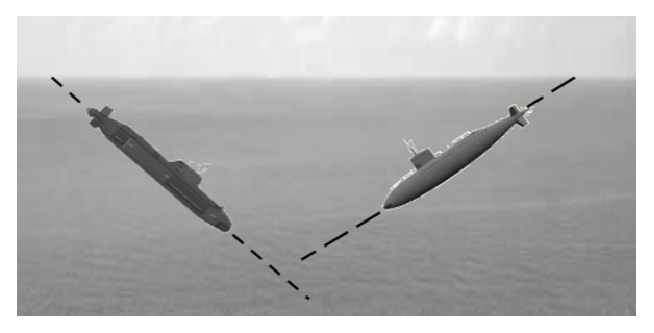
\includegraphics[scale=0.6]{Exo3_1}
\end{flushright}
\end{minipage}

Le plan défini par \Oij{} représente la surface de la mer. La cote $z$ est nulle au niveau de la
mer, négative sous l'eau.

\medskip

\begin{enumerate}
\item On admet que, pour tout réel $t \geqslant 0$, le point $S_1(t)$ a pour coordonnées:\index{equation parametrique@équation paramétrique}
\[\left\{\begin{array}{l c l}
x(t) &=& \phantom{-}140 - 60t\\
y(t) &=& \phantom{-}105 - 90t\\
z(t) &=& -170 - 30 t
\end{array}\right.\]

	\begin{enumerate}
		\item Donner les coordonnées du sous- marin au début de l'observation.
		\item Quelle est la vitesse du sous-marin ?
\item  On se place dans le plan vertical contenant la trajectoire du premier sous-marin.
		
\parbox{0.7\linewidth}{Déterminer l'angle $\alpha$ que forme la trajectoire du sous-marin avec le plan horizontal.
		
On donnera l'arrondi de $\alpha$ à $0,1$ degré près.}\hfill
\parbox{0.28\linewidth}{		
\begin{flushright}
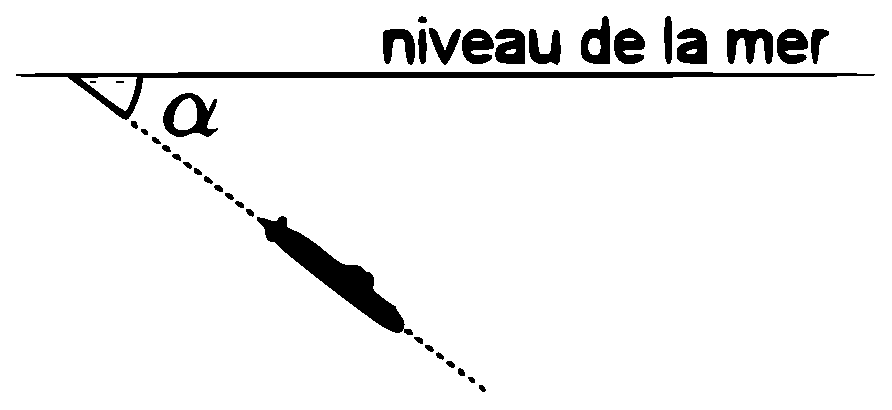
\includegraphics[scale=0.22]{Exo3_2}
\end{flushright}}

	\end{enumerate}
\item  Au début de l'observation, le second sous-marin est situé au point $S_2(0)$ de coordonnées
$(68~;~135~;~- 68)$ et atteint au bout de trois minutes le point $S_2(3)$ de coordonnées $(-202~;~-405~;~ - 248)$ avec une vitesse constante.

À quel instant $t$, exprimé en minutes, les deux sous-marins sont-ils à la même profondeur ?
\end{enumerate}

\vspace{0,5cm}

\textbf{EXERCICE 4 \hfill 5 points}

\textbf{Commun à tous les candidats}

\medskip

On considère, pour tout entier $n > 0$, les fonctions $f_n$ définies sur l'intervalle [1~;~5J par:

\[f_n(x) = \dfrac{\ln x}{x^n}.\]
 .
Pour tout entier $n > 0$, on note $\mathcal{C}_n$ la courbe représentative de la fonction $f_n$ dans un repère orthogonal.
 
Sur le graphique ci-dessous sont représentées les courbes $\mathcal{C}_n$ pour $n$ appartenant à 
 $\{1~;~2~;~3~;~4\}$.

\begin{center}
\psset{xunit=1.8cm,yunit=5cm,comma=true}
\begin{pspicture}(-0.2,-0.1)(5.2,0.7)
\psaxes[linewidth=1.25pt,Dy=0.5]{->}(0,0)(0,0)(5.2,0.7)
\psplot[plotpoints=300,linewidth=1.25pt,linecolor=blue]{1}{5}{x ln x div}
\psplot[plotpoints=300,linewidth=1.25pt,linecolor=red]{1}{5}{x ln x dup mul div}
\psplot[plotpoints=300,linewidth=1.25pt,linecolor=orange]{1}{5}{x ln x 3 exp  div}
\psplot[plotpoints=300,linewidth=1.25pt,linecolor=cyan]{1}{5}{x ln x 4 exp div}
\end{pspicture}
\end{center}

\medskip

\begin{enumerate}
\item Montrer que, pour tout entier $n > 0$ et tout réel $x$ de l'intervalle [1~;~5] :

\[f'_n(x) = \dfrac{1- n\ln (x)}{x^{n+1}}.\]\index{dérivée}

\item  Pour tout entier $n > 0$, on admet que la fonction $f_n$ admet un maximum sur l'intervalle [1~;~5].

On note $A_n$ le point de la courbe $\mathcal{C}_n$ ayant pour ordonnée ce maximum.\index{maximum}

Montrer que tous les points $A_n$ appartiennent à une même courbe $\Gamma$ d'équation

\[y = \dfrac{1}{\text{e}} \ln (x).\]

\item 
	\begin{enumerate}
		\item Montrer que, pour tout entier $n > 1$ et tout réel $x$ de l'intervalle [1~;~5] :

\[0 \leqslant \dfrac{\ln (x)}{x^n} \leqslant \dfrac{\ln (5)}{x^n}.\]
		
		\item  Montrer que pour tout entier $n > 1$ :
		
\[\displaystyle\int_1^5 \dfrac{1}{x^n} \:\text{d}x = \dfrac{1}{n - 1}\left(1 - \dfrac{1}{5^{n - 1}} \right).\]

		\item  Pour tout entier $n > 0$, on s'intéresse à l'aire, exprimée en unités d'aire, de la surface sous la courbe $f_n$, c'est-à-dire l'aire du domaine du plan délimité par les droites d'équations $x = 1$, $x = 5$, $y = 0$ et la courbe $\mathcal{C}_n$.\index{aire et intégrale}

Déterminer la valeur limite de cette aire quand $n$ tend vers $+ \infty$.
	\end{enumerate}
\end{enumerate}

\vspace{0.5cm}

\textbf{EXERCICE 5 \hfill 5 points}

\textbf{Candidats n'ayant pas suivi l'enseignement de spécialité}

\medskip

Un jeu de hasard sur ordinateur est paramétré de la façon suivante :\index{probabilité}

\medskip

\setlength\parindent{9mm}
\begin{itemize}
\item[$\bullet~~$]  Si le joueur gagne une partie, la probabilité qu'il gagne la partie suivante est 
$\dfrac{1}{4}$ ;
\item[$\bullet~~$] Si le joueur perd une partie, la probabilité qu'il perde la partie suivante est $\dfrac{1}{2}$ ;
\item[$\bullet~~$] La probabilité de gagner la première partie est $\dfrac{1}{4}$ .
\end{itemize}
\setlength\parindent{0mm}
\medskip

Pour tout entier naturel $n$ non nul, on note $G_n$ l'évènement \og la $n\up{e}$ partie est gagnée \fg{} et on note $p_n$ la probabilité de cet évènement. On a donc $p_1 = \dfrac{1}{4}$.
\medskip

\begin{enumerate}
\item Montrer que $p_2 = \dfrac{7}{16}$.
\item Montrer que, pour tout entier naturel $n$ non nul, $p_{n+1} = - \dfrac{1}{4}p_n + \dfrac{1}{2}$.
\item On obtient ainsi les premières valeurs de $p_n$ :

\begin{center}
\begin{tabularx}{0.8\linewidth}{|c|*{7}{>{\centering \arraybackslash}X|}}\hline
$n$ &1 &2 &3 &4 &5 &6 &7\\ \hline
$p_n$& 0,25 &\np{0,4375} &\np{0,3906} &\np{0,4023} &\np{0,3994} &\np{0,4001} &\np{0,3999}\\ \hline
\end{tabularx}
\end{center}

Quelle conjecture peut-on émettre ?
\item On définit, pour tout entier naturel $n$ non nul, la suite $\left(u_n\right)$ par $u_n = p_n - \dfrac{2}{5}$.\index{suite}
	\begin{enumerate}
		\item Démontrer que la suite $\left(u_n\right)$ est une suite géométrique dont on précisera la raison.\index{suite géométrique}
		\item En déduire que, pour tout entier naturel $n$ non nul, $p_n = \dfrac{2}{5} - \dfrac{3}{20}\left(- \dfrac{1}{4}\right)^{n-1}$.
		\item La suite $\left(p_n\right)$ converge-t-elle ? Interpréter ce résultat.
	\end{enumerate}
\end{enumerate}

\vspace{0.5cm}

\textbf{EXERCICE 5 \hfill 5 points}

\textbf{Candidats ayant suivi l'enseignement de spécialité}

\medskip

On définit la suite de réels $\left(a_n\right)$ par :
\[\left\{\begin{array}{l c l}
a_0 &= &0\\
a_1 &= &1\\
a_{n+1} &=& a_n + a_{n-1}\: \text{ pour }\: n \geqslant 1.
\end{array}\right.\]

On appelle cette suite la suite de Fibonacci.\index{suite}

\medskip

\begin{enumerate}
\item Recopier et compléter l'algorithme ci-dessous pour qu'à la fin de son exécution la variable $A$
contienne le terme $a_n$.\index{algorithme}

\begin{center}
\begin{tabularx}{0.4\linewidth}{|c X|}\hline
1&$A \gets 0$\\
2& $B \gets 1$\\
3& Pour $i$ allant de 2 à $n$ :\\
4& \multicolumn{1}{|l|}{\hspace{0.4cm} $C \gets A + B$}\\
5& \multicolumn{1}{|l|}{\hspace{0.4cm} $A \gets \ldots$}\\
6& \multicolumn{1}{|l|}{\hspace{0.4cm} $B \gets \ldots$}\\
7& Fin Pour\\ \hline
\end{tabularx}
\end{center}

On obtient ainsi les premières valeurs de la suite $a_n$ :

\begin{center}
\begin{tabularx}{\linewidth}{|c|*{11}{>{\centering \arraybackslash}X|}}\hline
$n$		&0 	&1 	&2 	&3 	&4 	&5 &6 	&7 		&8 	&9 &10\\ \hline
$a_n$	&0	& 1 &1	&2 	&3	&5 &8 	&13 	&21 &34 &55\\ \hline
\end{tabularx}
\end{center}
\item  Soit la matrice $A = \begin{pmatrix}1&1\\1&0\end{pmatrix}$.\index{matrice}

Calculer $A^2$, $A^3$ et $A^4$. 

Vérifier que $A^5 = \begin{pmatrix}8&5\\5&3\end{pmatrix}$.
\item On peut démontrer, et nous admettrons, que pour tout entier naturel $n$ non nul,

\[A^n = \begin{pmatrix}a_{n+1}&a_n\\a_n&a_{n-1}\end{pmatrix}.\]

	\begin{enumerate}
		\item Soit $p$ et $q$ deux entiers naturels non nuls. Calculer le produit $A^p \times A^q$ et en déduire que
		
		\[a_{p+q} = a_p \times a_{q+1} + a_{p-1} \times a_q.\]
		
		\item  En déduire que si un entier $r$ divise les entiers $a_p$ et $a_q$, alors $r$ divise également $a_{p+q}$.
		\item  Soit $p$ un entier naturel non nul.
		
Démontrer, en utilisant un raisonnement par récurrence sur $n$, que pour tout entier naturel
$n$ non nul, $a_p$ divise $a_{np}$.\index{récurrence}
	\end{enumerate}
\item 
	\begin{enumerate}
		\item Soit $n$ un entier supérieur ou égal à 5. Montrer que si $n$ est un entier naturel qui n'est pas premier, alors $a_n$ n'est pas un nombre premier.\index{nombre premier}
		\item On peut calculer $a_{19} = \np{4181} = 37 \times 113$.
		
Que penser de la réciproque de la propriété obtenue dans la question 4. a. ?
	\end{enumerate}
\end{enumerate}
%%%%%%%%%%%%   fin Liban 29 mai 2018
\newpage
%%%%%%%%%%%%   Amérique du Nord 29 mai 2018
\hypertarget{AmeriqueNord}{}

\label{AmeriqueNord}
\lfoot{\small{Amérique du Nord}}
\rfoot{\small 29 mai 2018}
\pagestyle{fancy}
\thispagestyle{empty}
\begin{center}\textbf{Durée : 4 heures}

\vspace{0,5cm}

{\Large \textbf{\decofourleft~Baccalauréat S Amérique du Nord 29 mai 2018~\decofourright}}
\end{center}

\vspace{0,5cm}

\textbf{Exercice 1 \hfill  6 points}

\textbf{Commun à  tous les candidats}

\medskip

On étudie certaines caractéristiques d'un supermarché d'une petite ville.

\bigskip

\textbf{Partie A - Démonstration préliminaire}

\medskip

Soit $X$ une variable aléatoire qui suit la loi exponentielle de paramètre $0,2$.\index{loi exponentielle}

On rappelle que l'espérance de la variable aléatoire $X$, notée $E(X)$, est égale à:

\[\displaystyle\lim_{x \to + \infty}\displaystyle\int_{0}^{x}  0,2t\text{e}^{-0,2t}\:\text{d}t.\]

Le but de cette partie est de démontrer que $E(X) = 5$.

\medskip

\begin{enumerate}
\item On note $g$ la fonction définie sur l'intervalle $[0~;~+\infty[$ par $g(t) = 0,2t\text{e}^{-0,2t}$.

On définit la fonction $G$ sur l'intervalle $[0~;~+\infty[$ par $G(t) = (- t - 5)\text{e}^{-0,2t}$.

Vérifier que $G$ est une primitive de $g$ sur l'intervalle $[0~;~+\infty[$.\index{primitive}
\item  En déduire que la valeur exacte de $E(X)$ est 5.

\emph{Indication : on pourra utiliser, sans le démontrer, le résultat suivant }:

\[\displaystyle\lim_{x \to + \infty} x \text{e}^{- 0,2x} = 0.\]
\end{enumerate}

\bigskip

\textbf{Partie B - Étude de la durée de présence d'un client dans le supermarché}

\medskip

Une étude commandée par le gérant du supermarché permet de modéliser la durée, exprimée en
minutes, passée dans le supermarché par un client choisi au hasard par une variable aléatoire $T$.

Cette variable $T$ suit une loi normale d'espérance $40$ minutes et d'écart type un réel positif noté $\sigma$.\index{loi normale}

Grâce à cette étude, on estime que $P(T < 10) = 0,067$.

\medskip

\begin{enumerate}
\item Déterminer une valeur arrondie du réel $\sigma$ à la seconde près.
\item Dans cette question, on prend $\sigma = 20$~minutes. Quelle est alors la proportion de clients qui
passent plus d'une heure dans le supermarché ?
\end{enumerate}

\bigskip

\textbf{Partie C - Durée d'attente pour le paiement}

\medskip

Ce supermarché laisse le choix au client d'utiliser seul des bornes automatiques de paiement ou
bien de passer par une caisse gérée par un opérateur.

\medskip

\begin{enumerate}
\item La durée d'attente à une borne automatique, exprimée en minutes, est modélisée par une
variable aléatoire qui suit la loi exponentielle de paramètre $0,2$~min$^{-1}$.\index{loi exponentielle}
	\begin{enumerate}
		\item Donner la durée moyenne d'attente d'un client à une borne automatique de paiement.
		\item Calculer la probabilité, arrondie à $10^{-3}$, que la durée d'attente d'un client à une borne automatique de paiement soit supérieure à $10$ minutes.
	\end{enumerate}
\item L'étude commandée par le gérant conduit à la modélisation suivante:
	
\setlength\parindent{9mm}
\begin{itemize}
\item[$\bullet~~$] parmi les clients ayant choisi de passer à une borne automatique, 86\,\% attendent moins de $10$ minutes ;
\item[$\bullet~~$] parmi les clients passant en caisse, 63\,\% attendent moins de $10$ minutes.
\end{itemize}
\setlength\parindent{0mm}

\medskip

On choisit un client du magasin au hasard et on définit les évènements suivants :

$B$ : \og le client paye à une borne automatique \fg{} ;

$\overline{B}$ : \og le client paye à une caisse avec opérateur \fg{} ;

$S$ : \og la durée d'attente du client lors du paiement est inférieure à $10$ minutes \fg.

Une attente supérieure à dix minutes à une caisse avec opérateur ou à une borne automatique
engendre chez le client une perception négative du magasin. Le gérant souhaite que
plus de 75\,\% des clients attendent moins de $10$ minutes.

Quelle est la proportion minimale de clients qui doivent choisir une borne automatique de
paiement pour que cet objectif soit atteint ?
 \end{enumerate}
 
\bigskip

\textbf{Partie D - Bons d'achat}

\medskip

Lors du paiement, des cartes à gratter, gagnantes ou perdantes, sont distribuées aux clients. Le
nombre de cartes distribuées dépend du montant des achats. Chaque client a droit à une carte à
gratter par tranche de $10$~\euro{} d'achats.

Par exemple, si le montant des achats est 58,64~\euro, alors le client obtient $5$ cartes ; si le montant est $124,31$~\euro, le client obtient $12$~cartes.

Les cartes gagnantes représentent $0,5$\,\% de l'ensemble du stock de cartes. De plus, ce stock est
suffisamment grand pour assimiler la distribution d'une carte à un tirage avec remise.

\medskip

\begin{enumerate}
\item Un client effectue des achats pour un montant de 158,02~\euro.

Quelle est la probabilité, arrondie à $10^{-2}$, qu'il obtienne au moins une carte gagnante ?\index{probabilité}
\item  À partir de quel montant d'achats, arrondi à 10~\euro, la probabilité d'obtenir au moins une carte
gagnante est-elle supérieure à 50\,\% ?
\end{enumerate}

\vspace{0,5cm}

\textbf{Exercice 2 \hfill  4 points}

\textbf{Commun à  tous les candidats}

\medskip

\parbox{0.6\linewidth}{Lors d'une expérience en laboratoire, on lance un projectile dans un milieu fluide. L'objectif est de déterminer pour quel angle de tir
$\theta$ par rapport à l'horizontale la hauteur du projectile ne dépasse
pas $1,6$ mètre.

Comme le projectile ne se déplace pas dans l'air mais dans un
fluide, le modèle parabolique usuel n'est pas adopté.

On modélise ici le projectile par un point qui se déplace, dans un
plan vertical, sur la courbe représentative de la fonction $f$ définie
sur l'intervalle [0~;~1[ par:

\[f(x) = bx + 2\ln (1- x)\]\index{fonction logarithme}

où $b$ est un paramètre réel supérieur ou égal à $2$, $x$ est l'abscisse
du projectile, $f(x)$ son ordonnée, toutes les deux exprimées en mètres.}
\hfill
\parbox{0.38\linewidth}{
\psset{unit=4cm,comma=true}
\begin{pspicture*}(-0.15,-0.15)(1.1,1.7)
\psgrid[gridlabels=0pt,subgriddiv=10,gridwidth=0.3pt,subgridwidth=0.15pt](0,0)(1.1,1.7)
\psaxes[linewidth=1pt,Dx=0.5,Dy=0.5,labelFontSize=\scriptstyle](0,0)(0,0)(1.1,1.7)
\psaxes[linewidth=1.5pt]{->}(0,0)(1,1)
\psplot[plotpoints=3000,linewidth=1.25pt,linecolor=blue]{0}{0.932}{5.69 x mul 1 x sub ln 2 mul add}
\psline[linestyle=dotted,linewidth=1pt](0.4,1.5)
\psarc(0,0){0.15}{0}{72}
\end{pspicture*}}

\medskip

\begin{enumerate}
\item La fonction $f$ est dérivable sur l'intervalle [0~;~1[. On note $f'$ sa fonction dérivée.

On admet que la fonction $f$ possède un maximum sur l'intervalle [0~;~1[ et que, pour tout réel
$x$ de l'intervalle [0~;~1[ :\index{maximum}

\[f'(x) = \dfrac{- bx + b - 2}{1 - x}.\]

Montrer que le maximum de la fonction $f$ est égal à $b - 2 + 2\ln \left(\dfrac{2}{b}\right)$.
\item  Déterminer pour quelles valeurs du paramètre $b$ la hauteur maximale du projectile ne dépasse
pas $1,6$~mètre.
\item  Dans cette question, on choisit $b = 5,69$.

L'angle de tir $\theta$ correspond à l'angle entre l'axe des abscisses et la tangente à la courbe de la
fonction $f$ au point d'abscisse $0$ comme indiqué sur le schéma donné ci-dessus.\index{tangente}

Déterminer une valeur approchée au dixième de degré près de l'angle $\theta$.
\end{enumerate}
 
\vspace{0,5cm}

\textbf{Exercice 3 \hfill  5 points}

\textbf{Commun à  tous les candidats}

\medskip

On se place dans l'espace muni d'un repère orthonormé dont l'origine est le point A.

On considère les points B$(10~;~-8~;~2)$, C$(-1~;~-8~;~5)$ et D(14~;~4~;~8).\index{géométrie dans l'espace}

\medskip

\begin{enumerate}
\item 
	\begin{enumerate}
		\item Déterminer un système d'équations paramétriques de chacune des droites (AB) et (CD).\index{equation parametrique@équation paramétrique}
		\item Vérifier que les droites (AB) et (CD) ne sont pas coplanaires.
	\end{enumerate}
\item On considère le point I de la droite (AB) d'abscisse 5 et le point J de la droite (CD) d'abscisse
4.
	\begin{enumerate}
		\item Déterminer les coordonnées des points I et J et en déduire la distance IJ.
		\item Démontrer que la droite (IJ) est perpendiculaire aux droites (AB) et (CD).
		
La droite (IJ) est appelée perpendiculaire commune aux droites (AB) et (CD).
 	\end{enumerate}
\item Cette question a pour but de vérifier que la distance IJ est la distance minimale entre les
droites (AB) et (CD).
	
Sur le schéma ci -dessous on a représenté les droites (AB) et (CD), les points I et J, et la droite
$\Delta$ parallèle à la droite (CD) passant par I.
	
On considère un point $M$ de la droite (AB) distinct du point I.
	
On considère un point $M'$ de la droite (CD) distinct du point J.
	
\begin{center}
\psset{unit=1cm}
\begin{pspicture}(12.3,7.8)
\pspolygon[fillstyle=solid,fillcolor=lightgray](0.7,1.2)(5.8,0.5)(11.5,3.8)(6.4,4.5)
%\psgrid
\psline(0,2)(12.3,2)%(AB)
\psline(1.5,0)(12.3,6)%\Delta
\psline(0,2.8)(10.8,8.8)%(CD)
\psline(5.1,2)(4.3,5.22)%IJ
\psline(7.3,3.22)(6.5,6.45)%PM'
\psline(7.3,3.22)(6.5,2)(6.5,6.45)%PMM'	
\uput[u](4.3,5.22){J}\uput[dr](5.1,2){I}
\uput[d](6.5,2){$M$}\uput[dr](7.3,3.22){$P$}
\uput[u](6.5,6.45){$M'$}
\uput[d](10.5,2){(AB)}\uput[ul](5.5,5.7){(CD)}
\uput[u](10,4.7){$\Delta$}
\psline(4.38,5)(4.55,5.07)(4.48,5.28)
\psline(5.08,2.258)(4.82,2.1)(4.88,1.9)
\end{pspicture}	
\end{center}

\medskip

	\begin{enumerate}
		\item Justifier que la parallèle à la droite (IJ) passant par le point $M'$ coupe la droite $\Delta$ en un point que l'on notera $P$.
		\item Démontrer que le triangle $MPM'$ est rectangle en $P$.
		\item Justifier que $MM' > IJ$ et conclure.
	\end{enumerate}
\end{enumerate}

\vspace{0,5cm}

\textbf{Exercice 4 \hfill  5 points}

\textbf{Candidats n'ayant pas suivi l'enseignement de spécialité}

\medskip

\textbf{Les deux graphiques donnés en annexe seront à compléter et à rendre avec la copie}

\medskip

Un scooter radio commandé se déplace en ligne droite à la vitesse constante de 1 m.s$^{-1}$. Il est poursuivi
par un chien qui se déplace à la même vitesse. 

On représente la situation vue de dessus dans un repère orthonormé du plan d'unité 1 mètre. L'origine de ce repère est la position initiale du chien. Le scooter est représenté par un point appartenant à la droite d'équation $x = 5$. Il se déplace sur cette droite dans le sens des ordonnées croissantes.

\smallskip

Dans la suite de l'exercice, on étudie deux modélisations différentes de la trajectoire du chien.

\bigskip

\textbf{Partie A - Modélisation à l'aide d'une suite}

\medskip

La situation est représentée par le graphique \no 1 donné en annexe.

À l'instant initial, le scooter est représenté par le point $S_0$. Le chien qui le poursuit est représenté
par le point $M_0$. On considère qu'à chaque seconde, le chien s'oriente instantanément en direction
du scooter et se déplace en ligne droite sur une distance de 1 mètre.

Ainsi, à l'instant initial, le chien s'oriente en direction du point $S_0$, et une seconde plus tard il se
trouve un mètre plus loin au point $M_1$. À cet instant, le scooter est au point $S_1$. Le chien s'oriente
en direction de $S_1$ et se déplace en ligne droite en parcourant 1 mètre, et ainsi de suite.

On modélise alors les trajectoires du chien et du scooter par deux suites de points notées $\left(M_n\right)$ et $\left(S_n\right)$.\index{suite}

Au bout de $n$ secondes, les coordonnées du point $S_n$ sont $(5~;~n)$. On note $\left(x_n~;~y_n\right)$ les coordonnées du point $M_n$.

\medskip

\begin{enumerate}
\item Construire sur le graphique \no 1 donné en annexe les points $M_2$ et $M_3$.
\item On note $d_n$ la distance entre le chien et le scooter $n$ secondes après le début de la poursuite.

On a donc $d_n = M_nS_n$.

Calculer $d_0$ et $d_1$.
\item  Justifier que le point $M_2$ a pour coordonnées $\left(1 + \dfrac{4}{\sqrt{17}}~;~\dfrac{1}{\sqrt{17}}\right)$.
\item  On admet que, pour tout entier naturel $n$ :\index{suite}

\[\left\{\begin{array}{l c l}
x_{n+1}& = &x_n + \dfrac{5 - x_n}{d_n}\\
y_{n+1}&=&y_n + \dfrac{n - y_n}{d_n}
\end{array}\right.\]

	\begin{enumerate}
		\item Le tableau ci-dessous, obtenu à l'aide d'un tableur, donne les coordonnées des points $M_n$
et $S_n$ ainsi que la distance $d_n$ en fonction de $n$. Quelles formules doit-on écrire dans les
cellules C5 et F5 et recopier vers le bas pour remplir les colonnes C et F ?\index{tableur}
		
\begin{center}
		\begin{tabularx}{\linewidth}{|c|*{6}{>{\centering \arraybackslash}X|}}\cline{2-7}
\multicolumn{1}{c|}{~}&A &B &C &D &E &F\\ \hline
1 &$n$& \multicolumn{2}{|c|}{$M_n$} & \multicolumn{2}{|c|}{$S_n$} &$d_n$\\ \hline
2 &&$x_n$& $y_n$& 5 &n&\\ \hline
3 &0& 0& 0& 5 &0& 5\\ \hline
4 &1 &1 &0 &5 &1 &\np{4,12310563}\\ \hline
5 &2 &\np{1,9701425} &\np{0,24253563} &5 &2 &\np{3,50267291}\\ \hline
6 &3 &\np{2,83515547} &\np{0,74428512} &5 &3 &\np{3,12646789}\\ \hline
7 &4 &\np{3,52758047} &\np{1,46577498} &5 &4 &\np{2,93092404}\\ \hline
\ldots&\ldots&\ldots&\ldots&\ldots&\ldots&\ldots\\ \hline
28 &24 &\np{4,99979751} &\np{21,2268342} &5 &24 &\np{2,7731658}\\ \hline
29 &25 &\np{4,99987053} &\np{22,2268342} &5 &25 &\np{2,7731658}\\ \hline
\end{tabularx}	
\end{center}

\medskip

		\item On admet que la suite $\left(d_n\right)$ est strictement décroissante.

Justifier que cette suite est convergente et conjecturer sa limite à l'aide du tableau.\index{limite de suite}
 	\end{enumerate}
\end{enumerate}
 
\bigskip
 
\textbf{Partie B - Modélisation à l'aide d'une fonction}
 
 \medskip
 
On modélise maintenant la trajectoire du chien à l'aide de la courbe $\mathcal{F}$ de la fonction $f$ définie pour tout réel $x$ de l'intervalle [0~;~5[ par:
 
\[f(x) = -2,5\ln (1 - 0, 2x) - 0,5x + 0,05x^2.\]\index{fonction logarithme}
 
 \medskip
 
Cela signifie que le chien se déplace sur la courbe $\mathcal{F}$ de la fonction $f$.
 
 \medskip
 
\begin{enumerate}
\item Lorsque le chien se trouve au point $M$ de coordonnées $(x~;~f(x))$ de la courbe $\mathcal{F}$, où $x$  appartient à l'intervalle [0~;~5[, le scooter se trouve au point $S$, d'ordonnée notée $y_S$. Ainsi le point $S$
a pour coordonnées $\left(5~;~y_S\right)$. La tangente à la courbe $\mathcal{F}$ au point $M$ passe par le point $S$. Cela traduit le fait que le chien s'oriente toujours en direction du scooter. On note $d(x)$ la distance $MS$ entre le chien et le scooter lorsque $M$ a pour abscisse $x$.
	\begin{enumerate}
		\item Sur le graphique \no 2 donné en annexe, construire, sans calcul, le point $S$ donnant la position du scooter lorsque le chien se trouve au point d'abscisse 3 de la courbe $\mathcal{F}$ et lire les
coordonnées du point $S$.
		\item On note $f'$ la fonction dérivée de la fonction $f$ sur l'intervalle [0~;~5[ et on admet que, pour tout réel $x$ de l'intervalle [0~;~5[ :

\[f'(x) = \dfrac{x(1  - 0,1x)}{5 - x}.\]\index{dérivée}

Déterminer par le calcul une valeur approchée au centième de l'ordonnée du point $S$ lorsque
le chien se trouve au point d'abscisse 3 de la courbe $\mathcal{F}$.
	\end{enumerate}
\item  On admet que $d(x) = 0,1x^2 - x + 5$ pour tout réel $x$ de l'intervalle [0~;~5[.

Justifier qu'au cours du temps la distance $MS$ se rapproche d'une valeur limite que l'on déterminera.\index{limite de fonction}
\end{enumerate}

\vspace{0,5cm}

\textbf{Exercice 4 \hfill  5 points}

\textbf{Candidats ayant suivi l'enseignement de spécialité}

\medskip

Dans une région, on s'intéresse à la cohabitation de deux espèces animales : les campagnols et les
renards, les renards étant les prédateurs des campagnols. 

Au 1\up{er} juillet 2012, on estime qu'il y a dans cette région approximativement deux millions de campagnols et cent-vingt renards.

On note $u_n$ le nombre de campagnols et $v_n$ le nombre de renards au 1\up{er} juillet de l'année $2012+ n$.\index{suite}

\bigskip

\textbf{Partie A - Un modèle simple}

\medskip

On modélise l'évolution des populations par les relations suivantes :

\[\left\{\begin{array}{l c r}
u_{n+1}& =& 1,1u_n - \np{2000}v_n\\
v_{n+1} &=& 2 \times 10^{-5}u_n + 0,6v_n
\end{array}\right. \quad \text{pour tout entier }\:n \geqslant 0,\: \text{avec } \:u_0 = \np{2000000}\:  \text{ et} \: v_0 = 120.\]\index{suite}

\medskip

\begin{enumerate}
\item 
	\begin{enumerate}
		\item On considère la matrice colonne $U_n = \begin{pmatrix}u_n\\v_n\end{pmatrix}$ pour tout entier $n \geqslant 0$.\index{matrice}
		
Déterminer la matrice $A$ telle que $U_{n+1} = A \times U_n$ pour tout entier $n$ et donner la matrice $U_0$.
		\item Calculer le nombre de campagnols et de renards estimés grâce à ce modèle au 1\up{er} juillet
2018.
	\end{enumerate}
\item Soit les matrices $P = \begin{pmatrix}\np{20000}&\np{5000}\\1&1\end{pmatrix}$, \:$D = \begin{pmatrix}1&0\\0&0,7\end{pmatrix}$ et $P^{-1} = \dfrac{1}{\np{15000}}\begin{pmatrix}1& \np{-5000}\\- 1&\np{20000}\end{pmatrix}$.
	
On admet que $P^{- 1}$ est la matrice inverse de la matrice $P$ et que $A = P \times D \times P^{- 1}$.\index{matrice inverse}
	\begin{enumerate}
		\item Montrer que pour tout entier naturel $n$,\: $U_n = P \times D^n \times P^{- 1} \times U_0$.
		\item Donner sans justification l'expression de la matrice $D^n$ en fonction de $n$.
		\item On admet que, pour tout entier naturel $n$ :
	
\renewcommand\arraystretch{1.8}	
\[\left\{\begin{array}{l c r}
u_n &=& \dfrac{2,8 \times 10^7 + 2 \times 10^6 \times 0,7^n}{15}\\

v_n &=&\dfrac{\np{1400} + 400 \times 0,7^n}{15}
		\end{array}\right.\]
\renewcommand\arraystretch{1}	
Décrire l'évolution des deux populations.
	\end{enumerate}
\end{enumerate}

\bigskip

\textbf{Partie B - Un modèle plus conforme à la réalité}

\medskip

Dans la réalité, on observe que si le nombre de renards a suffisamment baissé, alors le nombre de
campagnols augmente à nouveau, ce qui n'est pas le cas avec le modèle précédent. 

On construit donc un autre modèle, plus précis, qui tient compte de ce type d'observations à l'aide des relations suivantes :\index{suite}

\[\left\{\begin{array}{l c r}
u_{n+1} &=& 1,1u_n - 0,001u_n \times v_n\\
v_{n+1} &=& 2 \times 10^{-7} u_n \times v_n + 0,6v_n
\end{array}\right.\quad \text{pour tout entier }\:n \geqslant 0,\: \text{avec }\:u_0 = \np{2000000}\: \text{et }\: v_0 = 120.\]

\medskip

Le tableau ci-dessous présente ce nouveau modèle sur les $25$ premières années en donnant les
effectifs des populations arrondis à l'unité :
\begin{center}
\begin{tabularx}{0.7\linewidth}{|>{\columncolor[gray]{0.7}}c|*{3}{>{\centering \arraybackslash}X|}}\hline
\rowcolor[gray]{0.7}&A &B &C\\ \hline
1& \multicolumn{3}{c|}{Modèle de la \textbf{partie B}}\\ \hline
2& $n$ 	&$u_n$ 			&$v_n$\\ \hline
3&0		& \np{2000000} 	&120\\ \hline
4&1		& \np{1960000} 	&120\\ \hline
5&2		& \np{1920800} 	&119\\ \hline
6&3		& \np{1884228} 	&117\\ \hline
7&4		& \np{1851905} 	&114\\ \hline
8&5		& \np{1825160} 	&111\\ \hline
9&6		& \np{1804988} 	&107\\ \hline
10&7	& \np{1792049} 	&103\\ \hline
11&8	& \np{1786692} 	&99\\ \hline
12&9	& \np{1789005} 	&94\\ \hline
13&10	& \np{1798854} 	&91\\ \hline
14&11	& \np{1815930} 	&87\\ \hline
15&12	& \np{1839780} 	&84\\ \hline
16&13	& \np{1869827} 	&81\\ \hline
17&14	& \np{1905378} 	&79\\ \hline
18&15	& \np{1945622} 	&77\\ \hline
19&16	& \np{1989620} 	&77\\ \hline
20&17	& \np{2036288} 	&76\\ \hline
21&18	& \np{2084374} 	&77\\ \hline
22&19	& \np{2132440} 	&78\\ \hline
23&20	& \np{2178846} 	&80\\ \hline
24&21	& \np{2221746} 	&83\\ \hline
25&22	& \np{2259109} 	&87\\ \hline
26&23	& \np{2288766} 	&91\\ \hline
27&24	& \np{2308508} 	&97\\ \hline
\end{tabularx}
\end{center}

\medskip

\begin{enumerate}
\item Quelles formules faut-il écrire dans les cellules B4 et C4 et recopier vers le bas pour remplir
les colonnes B et C ?\index{tableur}
\item  Avec le deuxième modèle, à partir de quelle année observe-t-on le phénomène décrit (baisse
des renards et hausse des campagnols) ?
\end{enumerate}

\bigskip

\textbf{Partie C}

\medskip

Dans cette partie on utilise le modèle de la partie B.

Est - il possible de donner à $u_0$ et $v_0$ des valeurs afin que les deux populations restent stables d'une
année sur l'autre, c'est-à-dire telles que pour tout entier naturel $n$ on ait $u_{n+1} = u_n$ et $v_{n+1} = v_n$ ? (On parle alors d'état stable.)

\newpage

\begin{center}
\textbf{\large Annexe}

\vspace{1cm}

\textbf{À rendre avec la copie}
\vspace{1cm}
\textbf{EXERCICE 4}

\textbf{Candidats n'ayant pas suivi l'enseignement de spécialité}

\bigskip

\textbf{Partie A}, question 1

Graphique \no 1

\bigskip

\psset{unit=1.4cm}
\begin{pspicture}(-0.2,-0.2)(5.5,4.5)
\psgrid[gridlabels=0pt,subgriddiv=1](0,0)(5,4)
\psaxes[linewidth=1pt,labelFontSize=\scriptstyle](0,0)(0,0)(5.5,4.5)
\uput[dr](0,0){$M_0$}\uput[dr](1,0){$M_1$}\uput[ur](5,0){$S_0$}
\uput[ur](5,1){$S_1$}\uput[ur](5,2){$S_2$}\uput[ur](5,3){$S_3$}
\end{pspicture}

\vspace{1cm}

\textbf{Partie B}, question 1

Graphique \no 2

\bigskip

\psset{unit=1.4cm}
\begin{pspicture*}(-0.5,-0.5)(5.5,5.5)
\psgrid[gridlabels=0pt,subgriddiv=1,gridwidth=0.3pt](0,0)(5,6)
\psaxes[linewidth=1pt,labelFontSize=\scriptstyle](0,0)(0,0)(5.5,5.5)
\psaxes[linewidth=1.5pt,labelFontSize=\scriptstyle]{->}(0,0)(1,1)
\psplot[plotpoints=3000,linewidth=1.25pt,linecolor=blue]{0}{4.8}{0.05 x dup mul mul 0.5 x mul sub 1 0.2 x mul sub ln 2.5 mul sub}
\psdots(3,1.23)\uput[ul](3,1.23){$M$}\uput[l](4.5,5){\blue $\mathcal{F}$}
\end{pspicture*}
\end{center}
%%%%%%%%%%%%   fin Amérique du Nord 29 mai 2018
\newpage
%%%%%%%%%%%%   Centres étrangers 11 juin 2018
\hypertarget{Centresetrangers}{}

\label{Centresetrangers}
\lfoot{\small{Centres étrangers}}
\rfoot{\small{11 juin 2018}}
\pagestyle{fancy}
\thispagestyle{empty} 

\begin{center} {\Large{\textbf{\decofourleft~Baccalauréat S  Centres étrangers 11 juin 2018~\decofourright}}}
\end{center}

\textbf{Exercice 1\hfill 4 points}
 
\textbf{Pour tous les candidats}

\medskip

Dans une usine, on se propose de tester un prototype de hotte aspirante pour un local industriel.

Avant de lancer la fabrication en série, on réalise l'expérience suivante : dans un local clos équipé
du prototype de hotte aspirante, on diffuse du dioxyde de carbone (CO$_2$) à débit constant.

Dans ce qui suit, $t$ est le temps exprimé en minute.

À l'instant $t = 0$, la hotte est mise en marche et on la laisse fonctionner pendant $20$ minutes. Les
mesures réalisées permettent de modéliser le taux (en pourcentage) de CO$_2$ contenu dans le local au
bout de $t$ minutes de fonctionnement de la hotte par l'expression $f(t)$, où $f$ est la fonction définie
pour tout réel $t$ de l'intervalle [0~;~20] par :

\[f(t) = (0,8t + 0,2)\text{e}^{-0,5t} + 0,03.\]\index{fonction exponentielle}

\parbox{0.57\linewidth}{On donne ci-contre le tableau de variation de la fonction $f$ sur l'intervalle [0~;~20].

Ainsi, la valeur $f(0) = 0,23$ traduit le fait que le taux 
de CO$_2$ à l'instant $0$ est égal à 23\,\%.}\hfill
\parbox{0.41\linewidth}{\psset{unit=1.2cm}
\begin{pspicture}(5,2.5)
\psframe(5,2.5)\psline(0,1.5)(5,1.5)\psline(0,2)(5,2)\psline(1,0)(1,2.5)
\uput[u](0.5,1.9){$t$}\uput[u](1.1,1.9){$0$}\uput[u](3,1.9){$1,75$}\uput[u](4.8,1.9){$20$}
\rput(0.5,1.75){$f'(t)$}\rput(2,1.75){$+$}\rput(3,1.75){$0$}\rput(4,1.75){$-$}
\rput(0.5,0.75){$f$}\uput[u](1.3,0){\small $0,23$}
\psline{->}(1.5,0.5)(2.5,1.25)\psline{->}(3.5,1.25)(4.5,0.5)
\end{pspicture}}

\bigskip

\begin{enumerate}
\item Dans cette question, on arrondira les deux résultats au millième.
	\begin{enumerate}
		\item Calculer $f (20)$.
		\item Déterminer le taux maximal de CO$_2$ présent dans le local pendant l'expérience.
 	\end{enumerate}
\item  On souhaite que le taux de CO$_2$ dans le local retrouve une valeur $V$ inférieure ou égale à $3,5$\,\%.
	\begin{enumerate}
		\item Justifier qu'il existe un unique instant $T$ satisfaisant cette condition.
		\item On considère l'algorithme suivant :\index{algorithme}
		
\begin{center}
\begin{tabularx}{0.5\linewidth}{|X|}\hline
$t \gets 1,75$\\
$p \gets 0,1$\\
$V \gets 0,7$\\
Tant que $V > 0,035$\\
\hspace{0.75cm}$t \gets t + p$\\
\hspace{0.75cm}$V \gets (0,8t + 0,2)\text{e}^{-0,5t} + 0,03$\\
Fin Tant que\\ \hline
\end{tabularx}
\end{center}		
		
Quelle est la valeur de la variable $t$ à la fin de l'algorithme ?
		
Que représente cette valeur dans le contexte de l'exercice ?
 	\end{enumerate}
\item  On désigne par $V_m$ le taux moyen (en pourcentage) de CO$_2$ présent dans le local pendant les $11$
premières minutes de fonctionnement de la hotte aspirante.
	\begin{enumerate}
		\item Soit $F$ la fonction définie sur l'intervalle [0~;~11] par : 
		
		\[F(t) = (-1,6t -3,6)\text{e}^{-0,5t} +0,03t.\]
		
Montrer que la fonction $F$ est une primitive de la fonction $f$ sur l'intervalle [0~;~11].\index{primitive}
		\item En déduire le taux moyen $V_m$, valeur moyenne de la fonction $f$ sur l'intervalle [0~;~11].
Arrondir le résultat au millième, soit à $0,1$\,\%.\index{valeur moyenne}
	\end{enumerate}
\end{enumerate}

\textbf{Exercice 2\hfill 4 points}
 
\textbf{Pour tous les candidats}

\medskip

Pour chacune des quatre affirmations suivantes, indiquer si elle est vraie ou fausse, en justifiant la
réponse. Il est attribué un point par réponse exacte correctement justifiée. Une réponse inexacte ou
non justifiée ne rapporte ni n'enlève aucun point.\index{vrai-faux}

\bigskip

\begin{enumerate}
\item Un type d'oscilloscope a une durée de vie, exprimée en année, qui peut être modélisée par une
variable aléatoire $D$ qui suit une loi exponentielle de paramètre $\lambda$.

On sait que la durée de vie moyenne de ce type d'oscilloscope est de $8$ ans.

\smallskip

\textbf{Affirmation 1 :} pour un oscilloscope de ce type choisi au hasard et ayant déjà fonctionné $3$ ans,
la probabilité que la durée de vie soit supérieure ou égale à $10$ ans, arrondie au centième, est
égale à $0,42$.

\emph{On rappelle que si $X$ est une variable aléatoire qui suit une loi exponentielle de paramètre $\lambda$, on a pour tout réel $t$ positif :} $P(X \leqslant t) = 1 - \text{e}^{-\lambda t}$.
\item  En 2016, en France, les forces de l'ordre ont réalisé $9,8$ millions de dépistages d'alcoolémie
auprès des automobilistes, et 3,1\,\% de ces dépistages étaient positifs.\index{loi exponentielle}

Source : \emph{OFDT (Observatoire Français des Drogues et des Toxicomanies)}

Dans une région donnée, le 15 juin 2016, une brigade de gendarmerie a effectué un dépistage
sur $200$ automobilistes.

\smallskip

\textbf{Affirmation 2 :} en arrondissant au centième, la probabilité que, sur les $200$ dépistages, il y ait
eu strictement plus de $5$ dépistages positifs, est égale à $0,59$.
\item  On considère dans $\R$ l'équation :

\[\ln (6 x - 2) + \ln (2x - 1) = \ln (x).\]\index{fonction logarithme}

\smallskip

\textbf{Affirmation 3 :} l'équation admet deux solutions dans l'intervalle $\left]\dfrac{1}{2}~;~+ \infty\right[$.
\item  On considère dans $\C$ l'équation : 

\[\left(4z^2 - 20z + 37\right)(2z -7 + 2\text{i}) = 0.\]


\smallskip

\textbf{Affirmation 4 :} les solutions de l'équation sont les affixes de points appartenant à un même
cercle de centre le point P d'affixe $2$.\index{complexes}
\end{enumerate}

\textbf{Exercice 3\hfill 7 points}
 
\textbf{Pour tous les candidats}

\medskip

\emph{Les parties} A \emph{et} B \emph{sont indépendantes}

\medskip

Un détaillant en fruits et légumes étudie l'évolution de ses ventes de melons afin de pouvoir
anticiper ses commandes.

\bigskip

\textbf{Partie A}

\medskip

Le détaillant constate que ses melons se vendent bien lorsque leur masse est comprise entre $900$ g et
\np{1200}~g. Dans la suite, de tels melons sont qualifiés \og conformes \fg.

Le détaillant achète ses melons auprès de trois maraîchers, notés respectivement A, B et C.

Pour les melons du maraîcher A, on modélise la masse en gramme par une variable aléatoire $M_{\text{A}}$
qui suit une loi uniforme sur l'intervalle $[850~;~x]$, où $x$ est un nombre réel supérieur à \np{1200}.\index{loi uniforme}

La masse en gramme des melons du maraîcher B est modélisée par une variable aléatoire $M_{\text{B}}$ qui
suit une loi normale de moyenne \np{1050} et d'écart-type inconnu $\sigma$.\index{loi normale}

Le maraîcher C affirme, quant à lui, que 80\,\% des melons de sa production sont conformes.

\medskip

\begin{enumerate}
\item Le détaillant constate que 75\,\% des melons du maraîcher A sont conformes. Déterminer $x$.
\item Il constate que 85\,\% des melons fournis par le maraîcher B sont conformes.

Déterminer l'écart-type $\sigma$ de la variable aléatoire $M_{\text{B}}$. En donner la valeur arrondie à l'unité.\index{ecart-type@écart-type}
\item Le détaillant doute de l'affirmation du maraîcher C. Il constate que sur $400$ melons livrés par ce
maraîcher au cours d'une semaine, seulement $294$ sont conformes.

Le détaillant a-t-il raison de douter de l'affirmation du maraîcher C ?\index{intervalle de confiance}
\end{enumerate}

\bigskip

\textbf{Partie B}

\medskip

Le détaillant réalise une étude sur ses clients. Il constate que:

\begin{itemize}
\item parmi les clients qui achètent un melon une semaine donnée, 90\,\% d'entre eux achètent un
melon la semaine suivante;
\item parmi les clients qui n'achètent pas de melon une semaine donnée, 60\,\% d'entre eux n'achè\-tent
pas de melon la semaine suivante.
\end{itemize}

\smallskip

On choisit au hasard un client ayant acheté un melon au cours de la semaine 1 et, pour $n \geqslant 1$, on
note $A_n$ l'évènement : \og le client achète un melon au cours de la semaine $n$ \fg.

On a ainsi $p\left(A_1\right) = 1$.

\medskip

\parbox{0.6\linewidth}{\begin{enumerate}
\item 
	\begin{enumerate}
		\item Reproduire et compléter l'arbre de probabilités
ci-contre, relatif aux trois premières semaines.\index{probabilité}
		\item Démontrer que $p\left(A_3\right) = 0,85$.
		\item Sachant que le client achète un melon au cours
de la semaine 3, quelle est la probabilité qu'il en ait acheté un au cours de la semaine 2 ?
		
Arrondir au centième.\index{arbre}
	\end{enumerate}
\end{enumerate}
}\hfill 
\parbox{0.31\linewidth}{\pstree[treemode=R,nodesepA=0pt,nodesepB=3pt]{\TR{$A_1$~}}
{
   \pstree{\TR{$A_2$~}}
      {
      \TR{$A_3$} 
      \TR{$\overline{A_3}$}
      }

   \pstree{\TR{$\overline{A_2}$~} }
     {
     \TR{$A_3$} 
     \TR{$\overline{A_3}$}
     }
}
}
\medskip
	
Dans la suite, on pose pour tout entier $n \geqslant 1$ : \:$p_n = P\left(A_n\right)$. On a ainsi $p_1 = 1$.

\medskip

\begin{enumerate}[resume,start=2]
\item Démontrer que, pour tout entier $n \geqslant 1$ : $p_{n+1} = 0,5p_n + 0,4$.\index{suite}
\item 
	\begin{enumerate}
		\item Démontrer par récurrence que, pour tout entier $n \geqslant 1$ : $p_n > 0,8$.
		\item Démontrer que la suite $\left(p_n\right)$ est décroissante.
		\item La suite $\left(p_n\right)$ est-elle convergente ?
 	\end{enumerate}
\item On pose pour tout entier $n \geqslant 1$ : $v_n = p_n - 0,8$.
	\begin{enumerate}
		\item Démontrer que $\left(v_n\right)$ est une suite géométrique dont on donnera le premier terme $v_1$ et la raison.\index{suite géométrique}
		\item  Exprimer $v_n$ en fonction de $n$.
		
En déduire que, pour tout $n \geqslant 1$,\: $p_n = 0,8 + 0,2 \times  0,5^{n-1}$.
		\item  Déterminer la limite de la suite $\left(p_n\right)$.
	\end{enumerate}
\end{enumerate}

\textbf{Exercice 4\hfill 5 points}
 
\textbf{Candidats n'ayant pas suivi la spécialité mathématique}

\medskip

\parbox{0.54\linewidth}{La figure ci-contre représente un cube ABCDEFGH.\index{géométrie dans l'espace}

Les trois points I, J, K sont définis par les conditions
suivantes :

\begin{itemize}
\item I est le milieu du segment [AD] ;
\item J est tel que $\vect{\text{AJ}} = \dfrac{3}{4} \vect{\text{AE}}$ ;
\item K est le milieu du segment [FG].
\end{itemize}}
\hfill
\parbox{0.44\linewidth}{
\psset{unit=0.75cm}
\begin{pspicture}(-0.5,-0.5)(8,7.8)
\psframe(0,0)(4.5,4.5)%ABFE
\psline(4.5,0)(6.7,2.3)(6.7,6.8)(4.5,4.5)%BCGF
\psline(6.7,6.8)(2.2,6.8)(0,4.5)%GHE
\psline[linestyle=dashed](0,0)(2.2,2.3)(6.7,2.3)
\psline[linestyle=dashed](2.2,2.3)(2.2,6.8)
\uput[dl](0,0){A} \uput[dr](4.5,0){B} \uput[r](6.7,2.3){C} 
\uput[ur](2.2,2.3){D} \uput[l](0,4.5){E} \uput[r](4.5,4.5){F} 
\uput[r](6.7,6.8){G} \uput[u](2.2,6.8){H} \uput[ul](1.1,1.15){I} 
\uput[l](0,3.375){J} \uput[dr](5.6,5.65){K}
\psdots(1.1,1.15)(0,3.375)(5.6,5.65) 
\end{pspicture}
}

\bigskip

\textbf{Partie A}

\medskip

\begin{enumerate}
\item Sur la figure donnée en annexe, construire sans justifier le point d'intersection P du plan (IJK) et
de la droite (EH). On laissera les traits de construction sur la figure.\index{construction dans l'espace}
\item En déduire, en justifiant, l'intersection du plan (IJK) et du plan (EFG).
\end{enumerate}
 
\bigskip

\textbf{Partie B}

\medskip

On se place désormais dans le repère orthonormé $\left(\text{A}~;~\vect{\text{AB}}, \vect{\text{AD}}, \vect{\text{AE}}\right)$.

\medskip

\begin{enumerate}
\item 
	\begin{enumerate}
		\item Donner sans justification les coordonnées des points I, J et K.
		\item Déterminer les réels $a$ et $b$ tels que le vecteur $\vect{n} (4~;~a~;~b)$ soit orthogonal aux vecteurs $\vect{\text{IJ}}$ et $\vect{\text{IK}}$.\index{vecteur normal}
		\item  En déduire qu'une équation cartésienne du plan (IJK) est : $4x - 6y - 4z + 3 = 0$.\index{equation de plan@équation de plan}
	\end{enumerate}
\item 
	\begin{enumerate}
		\item Donner une représentation paramétrique de la droite (CG).\index{equation parametrique@équation paramétrique}
		\item Calculer les coordonnées du point N, intersection du plan (IJK) et de la droite (CG).
		\item Placer le point N sur la figure et construire en couleur la section du cube par le plan (IJK).\index{section plane}
	\end{enumerate}
\end{enumerate}

\bigskip

\textbf{Partie C}

\medskip

On note R le projeté orthogonal du point F sur le plan (IJK). Le point R est donc l'unique point du
plan (IJK) tel que la droite (FR) est orthogonale au plan (IJK).


On définit l'intérieur du cube comme l'ensemble des points $M(x~;~y~;~z)$ tels que $\left\{\begin{array}{l}
0 < x < 1\\
0 < y < 1\\
0 < z < 1
\end{array}\right.$

Le point R est-il à l'intérieur du cube ?

\textbf{Exercice 4\hfill 5 points}
 
\textbf{Candidats ayant suivi la spécialité mathématique}

\medskip

Le but de cet exercice est d'envisager une méthode de cryptage à clé publique d'une information
numérique, appelée système RSA, en l'honneur des mathématiciens Ronald Rivest, Adi Shamir et
Leonard Adleman, qui ont inventé cette méthode de cryptage en 1977 et l'ont publiée en 1978.

\smallskip

Les questions 1 et 2 sont des questions préparatoires, la question 3 aborde le cryptage, la question 4
le décryptage.

\bigskip

\begin{enumerate}
\item Cette question envisage de calculer le reste dans la division euclidienne par $55$ de certaines
puissances de l'entier $8$.
	\begin{enumerate}
		\item Vérifier que $8^7 \equiv 2 \mod 55$.\index{division euclidienne}
		
En déduire le reste dans la division euclidienne par $55$ du nombre $8^{21}$.
		\item Vérifier que $8^2 \equiv 9 \mod 55$, puis déduire de la question \textbf{a.} le reste dans la division
euclidienne par $55$ de $8^{23}$.
 	\end{enumerate}
\item  Dans cette question, on considère l'équation $(E)$\: $23 x - 40 y = 1$, dont les solutions sont des
couples $(x~;~y)$ d'entiers relatifs.\index{equation diophantienne@équation diophantienne}
	\begin{enumerate}
		\item Justifier le fait que l'équation $(E)$ admet au moins un couple solution.
		\item Donner un couple, solution particulière de l'équation $(E)$.
		\item Déterminer tous les couples d'entiers relatifs solutions de l'équation $(E)$.
		\item En déduire qu'il existe un unique entier $d$ vérifiant les conditions $0 \leqslant d < 40$ et $23 d \equiv  1 \mod 40$.
 	\end{enumerate}
\item  Cryptage dans le système RSA
	
Une personne A choisit deux nombres premiers $p$ et $q$, puis calcule les produits $N = p q$ et
$n = (p - 1)(q - 1)$. Elle choisit également un entier naturel $c$ premier avec $n$.\index{nombre premier}
	
La personne A publie le couple $(N~;~c)$, qui est une clé publique permettant à quiconque de lui
envoyer un nombre crypté.
	
Les messages sont numérisés et transformés en une suite d'entiers compris entre $0$ et $N -1$.
	
Pour crypter un entier $a$ de cette suite, on procède ainsi : on calcule le reste $b$ dans la division
euclidienne par $N$ du nombre $a^c$, et le nombre crypté est l'entier $b$.

\smallskip

Dans la pratique, cette méthode est sûre si la personne A choisit des nombres premiers $p$ et $q$
très grands, s'écrivant avec plusieurs dizaines de chiffres.\index{nombre premier}

On va l'envisager ici avec des nombres plus simples : $p = 5$ et $q = 11$.

La personne A choisit également $c = 23$.
	\begin{enumerate}
		\item Calculer les nombres $N$ et $n$, puis justifier que la valeur de $c$ vérifie la condition voulue.
		\item Un émetteur souhaite envoyer à la personne A le nombre $a = 8$.
		
Déterminer la valeur du nombre crypté $b$.
	\end{enumerate}
\item  Décryptage dans le système RSA

La personne A calcule dans un premier temps l'unique entier naturel $d$ vérifiant les conditions
$0 \leqslant d < n$ et $cd \equiv 1 \mod n$.

Elle garde secret ce nombre $d$ qui lui permet, et à elle seule, de
décrypter les nombres qui lui ont été envoyés cryptés avec sa clé publique.

Pour décrypter un nombre crypté $b$, la personne A calcule le reste $a$ dans la division euclidienne
par $N$ du nombre $b^d$, et le nombre en clair -- c'est-à-dire le nombre avant cryptage -- est le
nombre $a$.

On admet l'existence et l'unicité de l'entier $d$, et le fait que le décryptage fonctionne.

Les nombres choisis par A sont encore $p = 5$, $q = 11$ et $c = 23$.
	\begin{enumerate}
		\item Quelle est la valeur de $d$ ?
		\item En appliquant la règle de décryptage, retrouver le nombre en clair lorsque le nombre crypté
est $b = 17$.
	\end{enumerate}
\end{enumerate}

\newpage

\begin{center}
\textbf{\large Annexe (à rendre avec la copie)}

\vspace{3cm}

\psset{unit=1.5cm}
\begin{pspicture}(-0.5,-0.5)(8,7.8)
\psframe(0,0)(4.5,4.5)%ABFE
\psline(4.5,0)(6.7,2.3)(6.7,6.8)(4.5,4.5)%BCGF
\psline(6.7,6.8)(2.2,6.8)(0,4.5)%GHE
\psline[linestyle=dashed](0,0)(2.2,2.3)(6.7,2.3)
\psline[linestyle=dashed](2.2,2.3)(2.2,6.8)
\uput[dl](0,0){A} \uput[dr](4.5,0){B} \uput[r](6.7,2.3){C} 
\uput[ur](2.2,2.3){D} \uput[l](0,4.5){E} \uput[r](4.5,4.5){F} 
\uput[r](6.7,6.8){G} \uput[u](2.2,6.8){H} \uput[ul](1.1,1.15){I} 
\uput[l](0,3.375){J} \uput[dr](5.6,5.65){K}
\psdots(1.1,1.15)(0,3.375)(5.6,5.65) 
\end{pspicture}
\end{center}
%%%%%%%%%%%%   fin Centres étrangers 11 juin 2018
\newpage
%%%%%%%%%%%%   Antilles--Guyane 19 juin 2018
\hypertarget{Antilles}{}

\label{Antilles}
\lfoot{\small{Antilles-Guyane}}
\rfoot{\small{19 juin 2018}}
\pagestyle{fancy}
\thispagestyle{empty} 
\begin{center}
{\Large\textbf{\decofourleft~ Baccalauréat S Antilles-Guyane 19 juin 2018 
~\decofourright}}
\end{center}

\def\labelitemi{$\bullet$}

%: EXERCICE 1
\vspace{1cm}\textbf{\textsc{Exercice 1} \hfill 5 points}

\smallskip
\textsc{Commun à tous les candidats}

\bigskip

L'exploitant d'une forêt communale décide d'abattre des arbres afin de les vendre, soit aux habitants, soit à des entreprises. On admet que:
\begin{itemize}
\item parmi les arbres abattus, 30~\% sont des chênes, 50~\% sont des sapins et les autres sont des arbres d'essence secondaire (ce qui signifie qu'ils sont de moindre valeur);
\item \np{45,9}~\% des chênes et 80~\% des sapins abattus sont vendus aux habitants de la commune ;
\item les trois quarts des arbres d'essence secondaire abattus sont vendus à des entreprises. 
\end{itemize}

\medskip

\textbf{Partie A}

\smallskip

Parmi les arbres abattus, on en choisit un au hasard.

On considère les évènements suivants :\index{probabilité}
\begin{itemize}
\item $C$: \og l'arbre abattu est un chêne\fg{};
\item $S$: \og l'arbre abattu est un sapin\fg{};
\item $E$: \og l'arbre abattu est un arbre d'essence secondaire\fg{};
\item $H$: \og l'arbre abattu est vendu à un habitant de la commune\fg{}.
\end{itemize}

\medskip

\begin{enumerate}
\item Construire un arbre pondéré complet traduisant la situation.\index{arbre}
\item Calculer la probabilité que l'arbre abattu soit un chêne  vendu à un habitant de la commune.
\item Justifier que la probabilité que l'arbre abattu soit vendu à un habitant de la commune est égale à \np{0,5877}.
\item Quelle est la probabilité qu'un arbre abattu vendu à un habitant de la commune soit un sapin~?\\On donnera le résultat arrondi  à $10^{-3}$.
\end{enumerate}

\medskip

\textbf{Partie B}

\smallskip

Le nombre d'arbres sur un hectare de cette forêt peut être modélisé par une variable aléatoire $X$ suivant une loi normale d'espérance $\mu=\np{4000}$ et d'écart-type $\sigma=300$.\index{loi normale}

\medskip

\begin{enumerate}
\item Déterminer la probabilité qu'il y ait entre \np{3400} et \np{4600} arbres sur un hectare donné de cette forêt. On donnera le résultat arrondi à $10^{-3}$.
\item Calculer la probabilité qu'il y ait plus de \np{4500} arbres sur un hectare donné de cette forêt.
On donnera le résultat arrondi à $10^{-3}$.
\end{enumerate}

\medskip

\textbf{Partie C}

\smallskip

L'exploitant affirme que la densité de sapins dans cette forêt communale est de 1 sapin pour 2 arbres.

\smallskip

Sur une parcelle, on a compté $106$ sapins dans un échantillon de $200$ arbres.
Ce résultat remet-il en cause l'affirmation de l'exploitant~?\index{intervalle de fluctuation asymptotique}

%: EXERCICE 2
\vspace{1cm}\textbf{\textsc{Exercice 2} \hfill 5 points}

\smallskip
\textsc{Commun à tous les candidats}

\bigskip

Un artiste souhaite réaliser une sculpture composée d'un tétraèdre posé sur un cube de 6 mètres d'arête.

Ces deux solides sont représentés par le cube $ABCDEFGH$ et par le tétraèdre $SELM$ ci-dessous.\index{géométrie dans l'espace}

\begin{center}
\psset{unit=0.8cm}
\begin{pspicture}(0,0)(8,8)
\pstGeonode[PosAngle=-135](0,0){B}
\pstGeonode[PosAngle=135](0,4){F}
\pstGeonode[PosAngle=-45](4,0){C}
\pstGeonode[PosAngle=0](4,4){G}
\pstGeonode[PosAngle=45](2,2){A}
\pstTranslation[PosAngle=-45]{B}{A}{C}[D]
\pstTranslation[PosAngle=45]{B}{A}{G}[H]
\pstTranslation[PosAngle=45]{B}{A}{F}[E]
\pstHomO[HomCoef=0.166666666667,PosAngle=-45]{A}{B}[I]
\pstHomO[HomCoef=0.166666666667,PosAngle=-45]{A}{D}[J]
\pstHomO[HomCoef=0.166666666667,PosAngle=135]{A}{E}[K]
\psline(B)(C)(G)(F)(B)
\psline[linestyle=dashed](B)(A)(E)
\psline[linestyle=dashed](A)(D)
\psline(G)(H)(D)(C)
\pstHomO[HomCoef=.3333333,PosAngle=45]{E}{H}[M]
\pstHomO[HomCoef=.3333333,PosAngle=135]{E}{F}[L]
\pstInterLL[PosAngle=90]{B}{L}{M}{D}{S}
\psline(S)(L)(M)(S)
\psline(F)(L)
\psline(M)(H)
\psline[linestyle=dashed](L)(E)(S)
\psline[linestyle=dashed](E)(M)
\psline[linestyle=dashed](L)(B)(D)(M)
\psline[linecolor=red]{->}(A)(I)
\psline[linecolor=red]{->}(A)(J)
\psline[linecolor=red]{->}(A)(K)
\end{pspicture}
\end{center}

\medskip

On munit l'espace du repère orthonormé $\left(A~;~\vect{AI}, \vect{AJ}, \vect{AK}\right)$ tel que: $I\in[AB]$, $J\in[AD]$, $K\in[AE]$ et 

$AI=AJ=AK=1$, l'unité graphique représentant 1 mètre.

Les points $L$, $M$ et $S$ sont définis de la façon suivante:
\begin{itemize}
\item $L$ est le point tel que $\vect{FL}=\frac23\vect{FE}$;
\item $M$ est le point d'intersection du plan $(BDL)$ et de la droite $(EH)$;
\item $S$ est le point d'intersection des droites $(BL)$ et $(AK)$.\index{construction dans l'espace}
\end{itemize}

\medskip

\begin{enumerate}
\item Démontrer, sans calcul de coordonnées, que les droites $(LM)$ et $(BD)$ sont parallèles.
\item Démontrer que les coordonnées du point $L$ sont $(2~;~0~;~6)$.
\item 
	\begin{enumerate}
		\item Donner une représentation paramétrique de la droite $(BL)$.
		\item Vérifier que les coordonnées du point $S$ sont $(0~;~0~;~9)$.
	\end{enumerate}
\item Soit $\vect{n}$ le vecteur de coordonnées $(3~;~3~;~2)$.
	\begin{enumerate}
		\item Vérifier que $\vect{n}$ est normal au plan $(BDL)$.\index{vecteur normal}
		\item Démontrer qu'une équation cartésienne du plan $(BDL)$ est:\index{equation de plan@équation de plan}
\[
3x+3y+2z-18=0.
\]
		\item On admet que la droite $(EH)$ a pour représentation paramétrique:
\[
\left\{
\begin{array}{rcl}
x&=&0\\
y&=&s~~~~(s\in\R)\\
z&=&6
\end{array}
\right.
\]
Calculer les coordonnées du point $M$.
\end{enumerate}
\item Calculer le volume du tétraèdre $SELM$. On rappelle que le volume $V$ d'un tétraèdre est donné par la formule suivante:
\[
V=\frac13\times\text{Aire de la base}\times\text{Hauteur}.
\]
\item L'artiste souhaite que la mesure de l'angle $\widehat{SLE}$ soit comprise entre 55\up{o} et 60\up{o}.\\
Cette contrainte d'angle est-elle respectée~?\index{trigonométrie}
\end{enumerate}

%: EXERCICE 3
\vspace{1cm}\textbf{\textsc{Exercice 3 \hfill 5 points}}

\smallskip
\textsc{Commun à tous les candidats}

\bigskip

Un publicitaire souhaite imprimer le logo ci-dessous sur un T-shirt:

\begin{center}
\psset{xunit=2.0cm,yunit=2.0cm,algebraic=true,dimen=middle,dotstyle=o,dotsize=5pt 0,linewidth=1.6pt,arrowsize=3pt 2,arrowinset=0.25}
\begin{pspicture*}(-2.,-2.)(5.,1.)
\pscustom[linewidth=0.8pt,fillcolor=lightgray!60,fillstyle=solid]{\psplot{-1.57}{4.6}{EXP(-x)*(-COS(x)+SIN(x)+1.0)}\lineto(4.6,0)\psplot{4.6}{-1.57}{-EXP(-x)*COS(x)}\lineto(-1.57,0)\closepath}
\psplot[linewidth=2.pt,plotpoints=200]{-1.57}{4.6}{EXP(-x)*(-COS(x)+SIN(x)+1.0)}
\psplot[linewidth=2.pt,plotpoints=200]{-1.57}{4.6}{-EXP(-x)*COS(x)}
\end{pspicture*}
\end{center}

Il dessine ce logo à l'aide des courbes de deux fonctions $f$ et $g$ définies sur $\R$ par:
\[
f(x)=\e^{-x}(-\cos x+\sin x+1)\text{~~et~~}
g(x)=-\e^{-x}\cos x.
\]

On admet que les fonctions $f$ et $g$ sont dérivables sur $\R$.\index{trigonométrie}

\medskip
 
\textbf{Partie A — Étude de la fonction $f$}

\medskip

\begin{enumerate}
\item Justifier que, pour tout $x\in\R$:\[
-\e^{-x}\leqslant f(x)\leqslant 3\e^{-x}.\]
\item En déduire la limite de $f$ en $+\infty$.
\item Démontrer que, pour tout $x\in\R$, $f'(x)=\e^{-x}(2\cos x-1)$ où $f'$ est la fonction dérivée de $f$.\index{dérivée}
\item Dans cette question, on étudie la fonction $f$ sur l'intervalle $[-\pi~;~\pi]$.
	\begin{enumerate}
		\item Déterminer le signe de $f'(x)$ pour $x$ appartenant à l'intervalle $[-\pi~;~\pi]$.
		\item En déduire les variations de $f$ sur $[-\pi~;~\pi]$.
	\end{enumerate}
\end{enumerate}

\medskip

\textbf{Partie B — Aire du logo}

\smallskip

On note $\mathcal{C}_f$ et $\mathcal{C}_g$ les représentations graphiques des fonctions $f$ et $g$ dans un repère orthonormé \Oij. L'unité graphique est de 2 centimètres. Ces deux courbes sont tracées en ANNEXE.

\medskip

\begin{enumerate}
\item Étudier la position relative de la courbe $\mathcal{C}_f$ par rapport à la courbe $\mathcal{C}_g$ sur $\R$.
\item Soit $H$ la fonction définie sur $\R$ par:
\[
H(x)=\left(-\frac{\cos x}{2}-\frac{\sin x}{2}-1\right)\e^{-x}.\index{fonction exponentielle}
\]
On admet que $H$ est une primitive de la fonction $x\mapsto (\sin x+1)\e^{-x}$ sur $\R$.\index{primitive}

On note $\mathcal{D}$ le domaine délimité par la courbe $\mathcal{C}_f$, la courbe $\mathcal{C}_g$ est les droites d'équation $x=-\frac{\pi}{2}$ et $x=\frac{3\pi}{2}$.\index{aire et primitive}
	\begin{enumerate}
		\item Hachurer le domaine $\mathcal{D}$ sur le graphique en annexe à rendre avec la copie.
		\item Calculer, en unité d'aire, l'aire du domaine $\mathcal{D}$, puis en donner une valeur approchée à $10^{-2}$ près en cm\up{2}.
	\end{enumerate}
\end{enumerate}

\newpage

%: EXERCICE 4
\vspace{0,5cm}\textbf{\textsc{Exercice 4 \hfill 5 points}}

\smallskip
\textsc{Candidats n'ayant pas suivi l'enseignement de spécialité}

\bigskip

Le directeur d'une réserve marine a recensé \np{3000} cétacés dans cette réserve au 1\up{er} juin 2017. Il est inquiet car il sait que le classement de la zone en \og réserve marine\fg{} ne sera pas reconduit si le nombre de cétacés de cette réserve devient inférieur à \np{2000}.

\smallskip

Une étude lui permet d'élaborer un modèle selon lequel, chaque année :

\begin{itemize}
\item entre le 1\up{er} juin et le 31 octobre, 80 cétacés arrivent dans la réserve marine;
\item entre le 1\up{er} novembre et le 31 mai, la réserve subit une baisse de 5~\% de son effectif par rapport à celui du 31 octobre qui précède.
\end{itemize}

On modélise l'évolution du nombre de cétacés par une suite $(u_n)$. Selon ce modèle, pour tout entier naturel $n$, $u_n$ désigne le nombre de cétacés au 1\up{er} juin de l'année $2017+n$. On a donc $u_0 = \np{3000}$.\index{suite}

\medskip

\begin{enumerate}
\item Justifier que $u_1 = \np{2926}$.
\item Justifier que, pour tout entier naturel $n$, $u_{n+1}=\np{0,95}u_n+76$.
\item À l'aide d'un tableur, on a calculé les 8 premiers termes de la suite $(u_n)$. Le directeur a configuré le format des cellules pour que ne soient affichés que des nombres arrondis à l'unité.
\begin{center}
\begin{tabular}{|c|c|c|c|c|c|c|c|c|c|}\hline
\rowcolor{lightgray!50}		&A		&B			&C&D&E&F&G&H&I\\\hline
\cellcolor{lightgray!50}1	&$n$	&0			&1&2&3&4&5&6&7\\\hline
\cellcolor{lightgray!50}2	&$u_n$	&\np{3000}	&\np{2926}&\np{2856}&\np{2789}&\np{2725}&\np{2665}&\np{2608}&\np{2553}\\\hline
\end{tabular}
\end{center}

Quelle formule peut-on entrer dans la cellule C2 afin d'obtenir, par recopie vers la droite, les termes de la suite $\left(u_n\right)$~?
\item 
	\begin{enumerate}
		\item Démontrer que, pour tout entier naturel $n$, $u_n \geqslant \np{1520}$.
		\item Démontrer que la suite $\left(u_n\right)$ est décroissante.
		\item Justifier que la suite $\left(u_n\right)$ est convergente. On ne cherchera pas ici la valeur de la limite.
	\end{enumerate}
\item On désigne par $\left(v_n\right)$ la suite définie par, pour tout entier naturel $n$,\: $v_n=u_n-\np{1520}$.
\begin{enumerate}
\item Démontrer que la suite $\left(v_n\right)$ est une suite géométrique de raison \np{0,95} dont on précisera le premier terme.\index{suite géométrique}
\item En déduire que, pour tout entier naturel $n$, $u_n = \np{1480}\times\np{0,95}^n + \np{1520}$.
\item Déterminer la limite de la suite $\left(u_n\right)$.
\end{enumerate}
\item Recopier et compléter l'algorithme suivant pour déterminer l'année à partir de laquelle le nombre de cétacés présents dans la réserve marine sera inférieur à \np{2000}.
\begin{center}
\fbox{
\begin{minipage}{4cm}
$n\leftarrow 0$\\
$u\leftarrow\np{3000}$\\
Tant que \ldots\\
\phantom{xxxx}$n\leftarrow \ldots$\\
\phantom{xxxx}$u\leftarrow \ldots$\\
Fin de Tant que
\end{minipage}
}
\end{center}
La notation \og $\leftarrow$\fg{} correspond à une affectation de valeur, ainsi \og $n\leftarrow 0$\fg{} signifie \og Affecter à $n$ la valeur $0$\fg.
\item La réserve marine fermera-t-elle un jour~? Si oui, déterminer l'année de la fermeture.
\end{enumerate}

%: EXERCICE 4
\vspace{0,5cm}\textbf{\textsc{Exercice 4 \hfill 5 points}}

\smallskip

\textsc{Candidats ayant  suivi l'enseignement de spécialité}

\bigskip

Le droit de pêche dans une réserve marine est réglementé : chaque pêcheur doit posséder une carte d'accréditation annuelle. Il existe deux types de cartes :

\begin{itemize}
\item une carte de pêche dite \og libre \fg{} (le pêcheur n'est pas limité en nombre de poissons pêchés);
\item une carte de pêche dite \og avec quota \fg{} (le pêcheur ne doit pas dépasser une certaine quantité hebdomadaire de poisson).
\end{itemize}

\smallskip

On suppose que le nombre total de pêcheurs reste constant d'année en année.

On note, pour l'année $2017+n$:
\begin{itemize}
\item $\ell_n$ la proportion de pêcheurs possédant la carte de pêche libre ;
\item $q_n$ la proportion de pêcheurs possédant la carte de pêche avec quota.
\end{itemize}

On observe que:
\begin{itemize}
\item chaque année, 65~\% des possesseurs de la carte de pêche libres achète de nouveaux une carte de pêche libre l'année suivante;
\item Chaque année, 45~\% des possesseurs de la carte de pêche avec quota acheté une carte de pêche libre l'année suivante ;
\item En 2017, 40~\% des pêcheurs ont acheté une carte de pêche libre. On a donc $\ell_0=\np{0,4}$ et $q_0=\np{0,6}$.
\end{itemize}

On note, pour tout entier naturel $n$, $P_n=\begin{pmatrix}
\ell_n\\q_n
\end{pmatrix}$.\index{matrice}

\medskip

\begin{enumerate}
\item Démontrer que, pour tout entier naturel $n$, $P_{n+1}= MP_n$, où $M$ est la matrice carrée $\begin{pmatrix}
\np{0,65}&\np{0,45}\\
\np{0,35}&\np{0,55}
\end{pmatrix}$.\index{suite}
\item Calculer la proportion de pêcheurs achetant une carte de pêche avec quota en 2019.
\item Un logiciel de calcul formel donne les résultats ci-dessous :
\begin{center}
\begin{tabular}{cc}
\begin{tabular}{|c|l|}
\hline
\cellcolor{lightgray!50}\begin{tabular}{c}1\\$\circ$\end{tabular} & 
\begin{tabular}{l}
$M:=\{\{\np{0.65},\np{0,45}\},\{\np{0.35},\np{0.55}\}\}$\\
$\checkmark~~ M:=\begin{pmatrix}
0,65&0,45\\0,35&0,55
\end{pmatrix}$
\end{tabular}
\\
\hline
\cellcolor{lightgray!50}\begin{tabular}{c}2\\$\circ$\end{tabular} & 
\begin{tabular}{l}
$P_0:=\{\{ 0,4 \},\{ 0,6 \}\}$\\
$\checkmark~~ P_0:=\begin{pmatrix}
0,4\\0,6
\end{pmatrix}$
\end{tabular}
\\
\hline
\cellcolor{lightgray!50}\begin{tabular}{c}3\\$\circ$\end{tabular} & 
\begin{tabular}{l}
$Q:=\{\{ 9,1 \},\{ 7,$- 1$ \}\}$\\
$\checkmark~~ Q:=\begin{pmatrix}
9&1\\7&-1
\end{pmatrix}$
\end{tabular}
\\
\hline
\cellcolor{lightgray!50}\begin{tabular}{c}4\\$\circ$\end{tabular} & 
\begin{tabular}{l}
$T:=\{\{ 1/16,1/16 \},\{ 7/16,- 9/16 \}\}$\\
$\checkmark~~ T:=\begin{pmatrix}
\frac{1}{16}&\frac{1}{16}\\\frac{7}{16}&-\frac{9}{16}
\end{pmatrix}$\\[-0.5ex]\quad
\end{tabular}
\\
\hline
\end{tabular}
&
\begin{tabular}{|c|l|}
\hline
\cellcolor{lightgray!50}\begin{tabular}{c}5\\$\circ$\end{tabular} & 
\begin{tabular}{l}
$TQ$\\
$\rightarrow~~ \begin{pmatrix}
1&0\\0&1
\end{pmatrix}$
\end{tabular}
\\
\hline
\cellcolor{lightgray!50}\begin{tabular}{c}6\\$\circ$\end{tabular} & 
\begin{tabular}{l}
$QT$\\
$\rightarrow~~ \begin{pmatrix}
1&0\\0&1
\end{pmatrix}$
\end{tabular}
\\
\hline
\cellcolor{lightgray!50}\begin{tabular}{c}7\\$\circ$\end{tabular} & 
\begin{tabular}{l}
$D:=TMQ$\\
$\rightarrow~~ D:=\begin{pmatrix}
1&0\\0&\frac15
\end{pmatrix}$
\\[-0.5ex]\quad
\end{tabular}
\\
\hline
\end{tabular}
\end{tabular}
\end{center}

En vous appuyant sur les résultats précédents, répondre aux deux questions suivantes :
\begin{enumerate}
\item Justifier que $Q$ est une matrice inversible et préciser sa matrice inverse.\index{matrice inverse}

On notera $Q^{-1}$ la matrice inverse de $Q$.
\item Justifier que $M = QDQ^{-1}$ et démontrer que, pour tout entier naturel $n$ non nul :
\[M^n=QD^nQ^{-1}.\]
\end{enumerate}
\item On admet que, pour tout entier naturel $n$ non nul,
\[
M^n=\frac{1}{16}\begin{pmatrix}
9+7\times\np{0,2}^n&9-9\times\np{0,2}^n\\
7-7\times\np{0,2}^n&7+9\times\np{0,2}^n
\end{pmatrix}.
\]
\begin{enumerate}
\item
Démontrer que pour tout entier naturel $n$, $P_n = M^nP_0$.
\item Justifier que, pour tout entier naturel $n$:
\[
\ell_n =\frac{9}{16}-\frac{13}{80}\times\np{0,2}^n.
\]
\end{enumerate}
\item La proportion de pêcheurs achetant la carte de pêche libre dépassera-t-elle 60~\%~?
\end{enumerate}

\newpage

\begin{center}
\textbf{Exercice 3}

\vspace{1.5cm}

\psset{unit=1.85cm,algebraic=true}
\begin{pspicture*}(-2.5,-2.1)(5.1,3.1)
\psgrid[gridlabels=0pt,subgriddiv=1,gridwidth=0.25pt]
\psaxes[linewidth=1pt](0,0)(-2,-2.1)(5,3)
\psaxes[linewidth=1.5pt]{->}(0,0)(1,1)
\uput[d](0.5,0){$\vect{\imath}$}
\uput[l](0,0.5){$\vect{\jmath}$}
\psplot[plotpoints=3000,linewidth=1.25pt,linestyle=dashed]{-2}{5}{(1+sin(x)-cos(x))*2.71828^(-x)}
\uput[u](1.5,0.4){$\mathcal{C}_f$}
\psplot[plotpoints=3000,linewidth=1.25pt,linecolor=blue]{-2}{5}{-cos(x)*2.71828^(-x)}
\uput[d](1.5,0){\blue $\mathcal{C}_g$}
\end{pspicture*}
\end{center}
%%%%%%%%%%%%   fin Antilles--Guyane 19 juin 2018
\newpage
%%%%%%%%%%%%   Polynésie 20 juin 2018
\hypertarget{Polynesie}{}

\label{Polynesie}
\lfoot{\small{Polynésie}}
\rfoot{\small{20 juin 2018}}
\pagestyle{fancy}
\thispagestyle{empty} 

\begin{center} {\Large{\textbf{\decofourleft~Baccalauréat S Polynésie 20 juin 2018~\decofourright}}}
\end{center}

\vspace{0,5cm}

\textbf{\textsc{Exercice 1} \hfill 5 points}
 
\textbf{Commun à tous les candidats}

\medskip

\textbf{Rappel de connaissances :}

\medskip

L'intervalle de fluctuation asymptotique au seuil de 95\,\% est donné par la formule\index{intervalle de fluctuation asymptotique}

\[\left[p- 1,96\dfrac{\sqrt{p(1 - p)}}{\sqrt{n}}~;~p + 1,96\dfrac{\sqrt{p(1 + p)}}{\sqrt{n}}\right]\]

où $n$ désigne la taille de l'échantillon et $p$ la proportion des individus possédant le caractère étudié dans cette population. Les conditions de validité de cet intervalle sont les suivantes :

\[n \geqslant 30,\: np \geqslant 5,\: n(1 - p) \geqslant 5.\]

La municipalité d'une grande ville dispose d'un stock de DVD qu'elle propose en location aux usagers des différentes médiathèques de cette ville.

Afin de renouveler son offre de location, la municipalité décide de retirer des DVD de son stock.

Parmi les DVD retirés, certains sont défectueux, d'autres non.

Parmi les 6\,\% de DVD défectueux sur l'ensemble du stock, 98\,\% sont retirés.

On admet par ailleurs que parmi les DVD non défectueux, 92\,\% sont maintenus dans le stock; les autres sont retirés.

\medskip

\textbf{Les trois parties sont indépendantes.}

\bigskip

\textbf{Partie A}

\medskip

On choisit un DVD au hasard dans le stock de la municipalité.

On considère les évènements suivants:

\setlength\parindent{9mm}
\begin{itemize}
\item[$\bullet~~$] $D$ : \og le DVD est défectueux \fg{} ;
\item[$\bullet~~$] $R$ : \og le DVD est retiré du stock \fg.
\end{itemize}
\setlength\parindent{0mm}

On note $\overline{D}$ et $\overline{R}$ les évènements contraires respectifs des évènements $D$ et $R$.

\medskip

\begin{enumerate}
\item Démontrer que la probabilité de l'évènement $R$ est $0,134$.\index{probabilité}
\item Une association caritative contacte la municipalité dans l'objectif de récupérer l'ensemble des DVD qui sont retirés du stock. Un responsable de la ville affirme alors que parmi ces DVD retirés, plus de la moitié est composée de DVD défectueux.

Cette affirmation est-elle vraie ?\index{intervalle de fluctuation asymptotique}
\end{enumerate}

\bigskip

\textbf{Partie B}

\medskip

Une des médiathèques de la ville se demande si le nombre de DVD défectueux qu'elle possède
n'est pas anormalement élevé. Pour cela, elle effectue des tests sur un échantillon de $150 $~DVD de son propre stock qui est suffisamment important pour que cet échantillon soit assimilé à un tirage successif avec remise. Sur cet échantillon, on détecte $14$ DVD défectueux.

Peut-on rejeter l'hypothèse selon laquelle, dans cette médiathèque, 6\,\% des DVD sont défectueux ?\index{intervalle de fluctuation asymptotique}

\bigskip

\textbf{Partie C}

\medskip

Une partie du stock de DVD de la ville est constituée de DVD de films d'animation destinés au jeune public. On choisit un film d'animation au hasard et on note $X$ la variable aléatoire qui donne la durée, en minutes, de ce film. $X$ suit une loi normale d'espérance $\mu = 80$ min et d'écart-type $\sigma$.\index{loi normale}

De plus, on estime que $P(X \geqslant 92) = 0,10$.

\medskip

\begin{enumerate}
\item Déterminer le réel $\sigma$ et en donner une valeur approchée à $0,01$.
\item Un enfant regarde un film d'animation dont il ne connaît pas la durée. Sachant qu'il en a déjà vu une heure et demie, quelle est la probabilité que le film se termine dans les cinq minutes qui suivent ?
\end{enumerate}

\vspace{0,5cm}

\textbf{\textsc{Exercice 2} \hfill 6 points}
 
\textbf{Commun  à tous les candidats}

\medskip

Dans cet exercice, on s'intéresse au volume d'une ampoule basse consommation.

\bigskip

\textbf{Partie A - Modélisation de la forme de l'ampoule}

\medskip

Le plan est muni d'un repère orthonormé \Oij.

On considère les points A$(-1~;~1)$, B(0~;~1), C(4~;~3), D(7~;~0), E$(4~;~-3)$, F$(0~;~-1)$ et G$(- 1~;~- 1)$.

On modélise la section de l'ampoule par un plan passant par son axe de révolution à l'aide de la figure ci-dessous :
\begin{center}
\psset{unit=1cm,algebraic=true}
\begin{pspicture*}(-2,-3.5)(8,3.5)
\psgrid[gridlabels=0pt,subgriddiv=1,gridwidth=0.3pt]
\psaxes[linewidth=1pt,Dx=10,Dy=10](0,0)(-2,-3.5)(8,3.5)
\psaxes[linewidth=1.5pt,Dx=10,Dy=10]{->}(0,0)(1,1)
\uput[d](0.5,0){$\vect{\imath}$}
\uput[l](0,0.5){$\vect{\jmath}$}
\psline(-1,1)(0,1)\psline(-1,-1)(0,-1)
\psplot[linewidth=1pt,plotpoints=3000]{0}{4}{2-cos(x*3.141659/4)}
\psplot[linewidth=1pt,plotpoints=3000]{0}{4}{cos(x*3.141659/4)-2}
\psarc[linewidth=1pt](4,0){3}{-90}{90}
\psdots(-1,1)(0,1)(4,3)(7,0)(4,-3)(0,-1)(-1,-1)
\uput[dl](0,0){\small O}\uput[ul](-1,1){\small A}\uput[ur](0,1){\small B}\uput[u](4,3){\small C}
\uput[ur](7,0){\small D}\uput[d](4,-3){\small E}\uput[dr](0,-1){\small F}\uput[d](-1,-1){\small G}
\end{pspicture*}
\end{center}

\medskip

La partie de la courbe située au-dessus de l'axe des abscisses se décompose de la manière suivante:

\setlength\parindent{9mm}
\begin{itemize}
\item[$\bullet~~$] la portion située entre les points A et B est la représentation graphique de la fonction constante
$h$ définie sur l'intervalle $[-1~;~0]$ par $h(x) = 1$ ;
\item[$\bullet~~$] la portion située entre les points B et C est la représentation graphique d'une fonction $f$ définie sur l'intervalle [0~;~4] par $f(x) = a + b \sin \left(c + \frac{\pi}{4} x\right)$, où $a$, $b$ et $c$ sont des réels non nuls
fixés et où le réel $c$ appartient à l'intervalle $\left[0~;~\frac{\pi}{2}\right]$ ;
\item[$\bullet~~$] la portion située entre les points C et D est un quart de cercle de diamètre [CE].
\end{itemize}
\setlength\parindent{0mm}

La partie de la courbe située en-dessous de l'axe des abscisses est obtenue par symétrie par rapport à l'axe des abscisses.

\medskip

\begin{enumerate}
\item 
	\begin{enumerate}
		\item On appelle $f'$ la fonction dérivée de la fonction $f$. Pour tout réel $x$ de l'intervalle [0~;~4], déterminer $f'(x)$.\index{dérivée}
		\item On impose que les tangentes aux points B et C à la représentation graphique de la fonction $f$ soient parallèles à l'axe des abscisses. Déterminer la valeur du réel $c$.
	\end{enumerate}
\item  Déterminer les réels $a$ et $b$.
\end{enumerate}

\bigskip

\textbf{Partie B - Approximation du volume de l'ampoule}

\medskip

Par rotation de la figure précédente autour de l'axe des abscisses, on obtient un modèle de l'ampoule.

Afin d'en calculer le volume, on la décompose en trois parties comme illustré ci-dessous:

\begin{center}
\psset{unit=1cm,algebraic=true}
\begin{pspicture*}(-2,-4)(8,3.5)
%\psgrid[gridlabels=0pt,subgriddiv=1,gridwidth=0.3pt]
\psline(-1,1)(0,1)\psline(-1,-1)(0,-1)
\psplot[linewidth=1pt,plotpoints=3000]{0}{4}{2-cos(x*3.141659/4)}
\psplot[linewidth=1pt,plotpoints=3000]{0}{4}{cos(x*3.141659/4)-2}
\psarc[linewidth=1pt](4,0){3}{-90}{90}
\psdots(-1,1)(0,1)(4,3)(7,0)(4,-3)(0,-1)(-1,-1)
\uput[dl](0,0){\small O}\uput[ul](-1,1){\small A}\uput[ur](0,1){\small B}\uput[u](4,3){\small C}
\uput[ur](7,0){\small D}\uput[d](4,-3){\small E}\uput[dr](0,-1){\small F}\uput[d](-1,-1){\small G}
\pscustom[fillstyle=solid,fillcolor=lightgray]{
\psplot[linewidth=1pt,plotpoints=3000]{0}{4}{2-cos(x*3.141659/4)}
\psplot[linewidth=1pt,plotpoints=3000]{4}{0}{cos(x*3.141659/4)-2}}
\pscustom[fillstyle=crosshatch]{
\psline(4,3)(4,-3)\psarc[linewidth=1pt](4,0){3}{-90}{90}}
\psframe[fillstyle=hlines](-1,-1)(0,1)
\rput(3,-3.75){Vue dans le plan (BCE)}
\psaxes[linewidth=1pt,Dx=10,Dy=10](0,0)(-2,-3.5)(8,3.5)
\psaxes[linewidth=1.5pt,Dx=10,Dy=10]{->}(0,0)(1,1)
\uput[d](0.5,0){$\vect{\imath}$}
\uput[l](0,0.5){$\vect{\jmath}$}
\end{pspicture*}
\end{center}

\medskip

On rappelle que:

\setlength\parindent{9mm}
\begin{itemize}
\item[$\bullet~~$] le volume d'un cylindre est donné par la formule $\pi r^2 h$ où $r$ est le rayon du disque de base et $h$ est la hauteur ;
\item[$\bullet~~$] le volume d'une boule de rayon $r$ est donné par la formule $\dfrac{4}{3}\pi r^3$.
\end{itemize}
\setlength\parindent{0mm}

On admet également que, pour tout réel $x$ de l'intervalle [0~;~4], $f(x) = 2 - \cos \left(\frac{\pi}{4}x\right)$.

\medskip

\begin{enumerate}
\item Calculer le volume du cylindre de section le rectangle ABFG.
\item Calculer le volume de la demi-sphère de section le demi-disque de diamètre [CE].
\item Pour approcher le volume du solide de section la zone grisée BCEF, on partage le segment [OO$'$] en $n$ segments de même longueur $\dfrac{4}{n}$ puis on construit $n$ cylindres de même hauteur $\dfrac{4}{n}$.
	\begin{enumerate}
		\item \textbf{Cas particulier :} dans cette question uniquement on choisit $n = 5$.
		
Calculer le volume du troisième cylindre, grisé dans les figures ci-dessous, puis en donner
la valeur arrondie à $10^{-2}$.

\begin{center}
\psset{unit=1cm,algebraic=true}
\begin{pspicture*}(-2,-4)(8,3.5)
%\psgrid[gridlabels=0pt,subgriddiv=1,gridwidth=0.3pt]
\psaxes[linewidth=1pt,Dx=10,Dy=10](0,0)(-2,-3.5)(8,3.5)
\psline(-1,1)(0,1)\psline(-1,-1)(0,-1)
\psplot[linewidth=1pt,plotpoints=3000]{0}{4}{2-cos(x*3.141659/4)}
\psplot[linewidth=1pt,plotpoints=3000]{0}{4}{cos(x*3.141659/4)-2}
\psarc[linewidth=1pt](4,0){3}{-90}{90}
\psdots(-1,1)(0,1)(4,3)(7,0)(4,-3)(0,-1)(-1,-1)
\uput[dl](0,0){\small O}
\uput[dr](4,0){\small O$'$}
\uput[ur](0,1){\small B}\uput[u](4,3){\small C}
\uput[ur](7,0){\small D}\uput[d](4,-3){\small E}\uput[dr](0,-1){\small F}
%\uput[d](-1,-1){\small G}
\psframe[fillstyle=solid,fillcolor=lightgray](0,-1)(0.8,1)
\psframe[fillstyle=solid,fillcolor=lightgray](0.8,-1.2)(1.6,1.2)
\psframe[fillstyle=solid,fillcolor=gray](1.6,-1.7)(2.4,1.7)
\psframe[fillstyle=solid,fillcolor=lightgray](2.4,-2.3)(3.2,2.3)
\psframe[fillstyle=solid,fillcolor=lightgray](3.2,-2.8)(4,2.8)
\rput(3,-3.8){Vue dans le plan (BCE)}
\psline(-1,-1)(-1,1)\psline(4,3)(4,-3)
\psaxes[linewidth=1.25pt,Dx=10,Dy=10]{->}(0,0)(1,1)
\uput[d](0.5,0){$\vect{\imath}$}
\uput[l](0,0.5){$\vect{\jmath}$}
\end{pspicture*}
\end{center}

\medskip

\begin{center}
\psset{unit=1cm,algebraic=true}
\begin{pspicture*}(-2,-4)(8,3.5)
%\psgrid
\psline(-1,1)(0,1)\psline(-1,-1)(0,-1)
\psplot[linewidth=1pt,plotpoints=3000]{0}{4}{2-cos(x*3.141659/4)}
\psplot[linewidth=1pt,plotpoints=3000]{0}{4}{cos(x*3.141659/4)-2}
\psarc[linewidth=1pt](4,0){3}{-90}{90}
\rput(3,-3.8){Vue dans l'espace}
\psline(-1,-1)(-1,1)
\psframe[fillstyle=solid,fillcolor=lightgray,linewidth=0pt](3.2,-2.8)(4,2.8)
\psellipse[fillstyle=solid,fillcolor=lightgray,linewidth=0pt](3.2,0)(0.3,2.8)
\psellipse[fillstyle=solid,fillcolor=lightgray,linewidth=0pt](4,0)(0.3,2.8)
\psframe[fillstyle=solid,fillcolor=lightgray,linewidth=0pt](2.4,-2.3)(3.2,2.3)
\psellipse[fillstyle=solid,fillcolor=lightgray,linewidth=0pt](2.4,0)(0.3,2.3)
\psellipse[fillstyle=solid,fillcolor=lightgray,linewidth=0pt](3.2,0)(0.3,2.3)
\psframe[fillstyle=solid,fillcolor=lightgray,linewidth=0pt](0.8,-1.2)(1.6,1.2)
\psellipse[fillstyle=solid,fillcolor=lightgray,linewidth=0pt](0.8,0)(0.3,1.2)
\psellipse[fillstyle=solid,fillcolor=lightgray,linewidth=0pt](1.6,0)(0.3,1.2)
\psframe[fillstyle=solid,fillcolor=lightgray,linewidth=0pt](0,-1)(0.8,1)
\psellipse[fillstyle=solid,fillcolor=lightgray,linewidth=0pt](0,0)(0.3,1)
\psellipse[fillstyle=solid,fillcolor=lightgray,linewidth=0pt](0.8,0)(0.3,1)
\psframe[fillstyle=solid,fillcolor=gray,linewidth=0pt](1.6,-1.7)(2.4,1.7)
\psellipse[fillstyle=solid,fillcolor=gray,linewidth=0pt](1.6,0)(0.3,1.7)
\psellipse[fillstyle=solid,fillcolor=gray,linewidth=0pt](2.4,0)(0.3,1.7)
\end{pspicture*}
\end{center}

		\item \textbf{Cas général :} dans cette question, $n$ désigne un entier naturel quelconque non nul.

On approche le volume du solide de section BCEF par la somme des volumes des $n$ cylindres
ainsi créés en choisissant une valeur de $n$ suffisamment grande.

Recopier et compléter l'algorithme suivant de sorte qu'à la fin de son exécution, la variable $V$ contienne la somme des volumes des $n$ cylindres créés lorsque l'on saisit $n$.\index{algorithme}

\begin{center}
\begin{tabularx}{0.45\linewidth}{|l X|}\hline
1&$V \gets 0$\\
2& Pour $k$ allant de \ldots à \ldots :\\
3& \hspace{0.5cm}| $V \gets \ldots$\\
4& Fin Pour\\ \hline
\end{tabularx}
\end{center}
	\end{enumerate}
\end{enumerate}
\vspace{0,5cm}

\textbf{\textsc{Exercice 3} \hfill 4 points}
 
\textbf{Commun  à tous les candidats}

\medskip

On considère la fonction $f$ définie sur l'intervalle $[0~;~ +\infty[$ par $f(x) = k\text{e}^{-kx}$  où $k$ est un nombre réel strictement positif.

On appelle $\mathcal{C}_f$ sa représentation graphique dans le repère orthonormé \Oij.

On considère le point A de la courbe $\mathcal{C}_f$ d'abscisse 0 et le point B de la courbe $\mathcal{C}_f$ d'abscisse 1.

Le point C a pour coordonnées (1~;~0).

\begin{center}
\psset{unit=3cm}
\begin{pspicture}(-0.2,-0.1)(2.2,2)
\psaxes[linewidth=1.pt,Dx=10,Dy=10](0,0)(0,0)(2.2,2)
\psaxes[linewidth=1.5pt,Dx=10,Dy=10]{->}(0,0)(1,1)
\pscustom[fillstyle=hlines]{
\psplot[plotpoints=3000,linewidth=1.25pt,linecolor=blue]{0}{1}{1.5 2.71828 1.5 x mul exp div}
\psline(1,0.335)(0,0)}
\rput(0.3,0.4){$\mathcal{D}$}
\rput(0.2,1.5){\blue $\mathcal{C}_f$}
\uput[d](0.5,0){$\vect{\imath}$}
\uput[l](0,0.5){$\vect{\jmath}$}
\psdots(0,1.5)(1,0.335)(1,0)%ABC
\uput[l](0,1.5){A}\uput[u](1,0.335){B}\uput[d](1,0){C}
\psline(1,0.335)(1,0)
\psplot[plotpoints=3000,linewidth=1.25pt,linecolor=blue]{0}{2.2}{1.5 2.71828 1.5 x mul exp div}
\end{pspicture}
\end{center}

\medskip

\begin{enumerate}
\item Déterminer une primitive de la fonction $f$ sur l'intervalle $[0~;~ +\infty[$.\index{primitive}
\item Exprimer, en fonction de $k$, l'aire du triangle OCB et celle du domaine $\mathcal{D}$ délimité par l'axe des ordonnées, la courbe $\mathcal{C}_f$ et le segment [OB].
\item Montrer qu'il existe une unique valeur du réel $k$ strictement positive telle que l'aire du domaine $\mathcal{D}$ vaut le double de celle du triangle OCB.
\end{enumerate}

\vspace{0,5cm}

\textbf{\textsc{Exercice 4} \hfill 5 points}
 
\textbf{Candidats n'ayant pas suivi l'enseignement de spécialité}

\medskip

Un lapin se déplace dans un terrier composé de trois galeries, notées A, B et C, dans chacune desquelles il est confronté à un stimulus particulier.

À chaque fois qu'il est soumis à un stimulus, le lapin reste dans la galerie où il se trouve ou change de galerie. Cela constitue une étape.

\smallskip

Soit $n$ un entier naturel.

On note $a_n$ la probabilité de l'évènement : \og le lapin est dans la galerie A à l'étape $n$ \fg.
On note $b_n$ la probabilité de l'évènement : \og le lapin est dans la galerie B à l'étape $n $\fg.
On note $c_n$ la probabilité de l'évènement : \og le lapin est dans la galerie C à l'étape $n $\fg.

À l'étape $n = 0$, le lapin est dans la galerie A.

Une étude antérieure des réactions du lapin face aux différents stimuli permet de modéliser ses déplacements par le système suivant :

\[\renewcommand\arraystretch{1.5}\left\{\begin{array}{l c r}
a_{n+1}&=&\frac{1}{3}a_n + \frac{1}{4} b_n \phantom{+ \frac{2}{3}c_n}\\
b_{n+1}&=&\frac{2}{3}a_n + \frac{1}{2} b_n + \frac{2}{3}c_n\\
c_{n+1}&=&\frac{1}{4}b_n + \frac{1}{3} c_n
\end{array}\right.\]

\medskip

L'objectif de cet exercice est d'estimer dans quelle galerie le lapin a la plus grande probabilité de se trouver à long terme.\index{probabilité}

\bigskip

\textbf{Partie A}

\medskip

À l'aide d'un tableur, on obtient le tableau de valeurs suivant:\index{tableur}

\begin{center}
\begin{tabularx}{0.75\linewidth}{|c|*{4}{>{\centering \arraybackslash}X|}}\hline
	&A &B &C &D\\ \hline
1 	&$n$ &$a_n$ &$b_n$ &$c_n$\\ \hline
2 	&0	& 1 	&0	&0\\ \hline
3	&1	&0,333 	&0,667 	&0\\ \hline
4 	&2 	&0,278 &0,556 &0,167\\ \hline
5 	&3 &0,231 &0,574 &0,194\\ \hline
6 	&4 &0,221 &0,571 &0,208\\ \hline
7 	&5 &0,216 &0,572 &0,212\\ \hline
8 	&6 &0,215 &0,571 &0,214\\ \hline
9 	&7 &0,215 &0,571 &0,214\\ \hline
10 	&8 &0,214 &0,571 &0,214\\ \hline
11 	&9 &0,214 &0,571 &0,214\\ \hline
12 	&10 &0,214 &0,571 &0,214\\ \hline
\end{tabularx}
\end{center}

\medskip

\begin{enumerate}
\item Quelle formule faut-il entrer dans la cellule C3 et recopier vers le bas pour remplir la colonne C ?
\item Quelle conjecture peut-on émettre ?
\end{enumerate}

\bigskip

\textbf{Partie B}

\medskip

\begin{enumerate}
\item On définit la suite $\left(u_n\right)$, pour tout entier naturel $n$, par $u_n = a_n - c_n$.\index{suite}
	\begin{enumerate}
		\item Démontrer que la suite $\left(u_n\right)$ est géométrique en précisant sa raison.\index{suite géométrique}
		\item Donner, pour tout entier naturel $n$, l'expression de $u_n$ en fonction de $n$.
	\end{enumerate}
\item  On définit la suite $\left(v_n\right)$ par $v_n = b_n - \dfrac{4}{7}$ pour tout entier naturel $n$.
	\begin{enumerate}
		\item Expliquer pourquoi pour tout entier naturel $n$,\: $a_n + b_n + c_n = 1$ et en déduire que pour tout entier naturel $n$,\: $v_{n+1} = - \dfrac{1}{6}v_n$.
		\item En déduire, pour tout entier naturel $n$, l'expression de $v_n$ en fonction de $n$.
	\end{enumerate}
\item  En déduire que pour tout entier naturel $n$, on a :

\[a_{n} = \dfrac{3}{14} +\dfrac{1}{2}\left(\dfrac{1}{3}\right)^n + \dfrac{2}{7}\left(- \dfrac{1}{6}\right)^n, \quad b_{n} = \dfrac{4}{7} - \dfrac{4}{7}\left(- \dfrac{1}{6}\right)^n \quad \text{et} \quad c_{n} = \dfrac{3}{14} -\dfrac{1}{2}\left(\dfrac{1}{3}\right)^n + \dfrac{2}{7}\left(- \dfrac{1}{6}\right)^n.\]

\item  Que peut-on en déduire sur la position du lapin après un très grand nombre d'étapes ?
\end{enumerate}
\vspace{0,5cm}

\textbf{\textsc{Exercice 4} \hfill 5 points}
 
\textbf{Candidats ayant  suivi l'enseignement de spécialité}

\medskip

Un atome d'hydrogène peut se trouver dans deux états différents, l'état stable et l'état excité. À chaque nanoseconde, l'atome peut changer d'état.

\bigskip

\textbf{Partie A - Étude d'un premier milieu}

\medskip

Dans cette partie, on se place dans un premier milieu (milieu 1) où, à chaque nanoseconde, la probabilité qu'un atome passe de l'état stable à l'état excité est $0,005$, et la probabilité qu'il passe de l'état excité à l'état stable est $0,6$.\index{probabilité}

On observe un atome d'hydrogène initialement à l'état stable.

On note $a_n$ la probabilité que l'atome soit dans un état stable et $b_n$ la probabilité qu'il se trouve dans un état excité, $n$ nanosecondes après le début de l'observation.

On a donc $a_0 = 1$ et $b_0 = 0$.

On appelle $X_n$ la matrice ligne $X_n = \begin{pmatrix}a_n& b_n\end{pmatrix}$.\index{matrice}

L'objectif est de savoir dans quel état se trouvera l'atome d'hydrogène à long terme.

\medskip

\begin{enumerate}
\item Calculer $a_1$ puis $b_1$ et montrer que $a_2 = \np{0,993025}$ et $b_2 = \np{0,006975}$.
\item Déterminer la matrice $A$ telle que, pour tout entier naturel $n$,\: $X_{n+1} = X_n A$.

$A$ est appelée matrice de transition dans le milieu 1.\index{matrice de transition}

On admet alors que, pour tout entier naturel $n$,\: $X_n = X_0A^n$.

\item On définit la matrice $P$ par $P = \begin{pmatrix}1&-1\\ 1&120\end{pmatrix}$.

On admet que $P$ est inversible et que
\[P^{-1} = \dfrac{1}{121}\begin{pmatrix}120&1\\- 1&1\end{pmatrix}.\]

Déterminer la matrice $D$ définie par $D = P^{-1} AP$.
\item Démontrer que, pour tout entier naturel $n$,\: $A^n = P D^n P^{-1}$.
\item On admet par la suite que, pour tout entier naturel $n$,

\[A^n = \dfrac{1}{121}\begin{pmatrix}120 + 0,395^n&1 - 0,395^n\\120\left(1 - 0,395^n\right)&1 + 120 \times 0,395^n\end{pmatrix}.\]

En déduire une expression de $a_n$ en fonction de $n$.
\item Déterminer la limite de la suite $\left(a_n\right)$. Conclure.\index{limite de suite}
\end{enumerate}

\bigskip

\textbf{Partie B - Étude d'un second milieu}

\medskip

Dans cette partie, on se place dans un second milieu (milieu 2), dans lequel on ne connaît pas la probabilité que l'atome passe de l'état excité à l'état stable. On note $a$ cette probabilité supposée constante. On sait, en revanche, qu'à chaque nanoseconde, la probabilité qu'un atome passe de l'état stable à l'état excité est $0,01$.

\medskip

\begin{enumerate}
\item Donner, en fonction de $a$, la matrice de transition $M$ dans le milieu 2.\index{matrice de transition}
\item Après un temps très long, dans le milieu 2, la proportion d'atomes excités se stabilise autour de 2\,\%.

On admet qu'il existe un unique vecteur $X$, appelé état stationnaire, tel que $XM = X$, et que $X = \begin{pmatrix}0,98& 0,02\end{pmatrix}$.

Déterminer la valeur de $a$.
\end{enumerate}
%%%%%%%%%%%%   fin Polynésie 20 juin 2018
\newpage
%%%%%%%%%%%%   Asie 21 juin 2018
\hypertarget{Asie}{}

\label{Asie}
\lfoot{\small{Asie}}
\rfoot{\small{21 juin 2018}}
\pagestyle{fancy}
\thispagestyle{empty} 

\begin{center} {\Large{\textbf{\decofourleft~Baccalauréat S -- Asie 21 juin 2018~\decofourright}}}
\end{center}

\vspace{0,5cm}

%\subsection*{\textsc{Exercice 1} \hfill 5 points}
\textbf{\textsc{\bf Exercice 1} \hfill 5 points}
 
\medskip
 
\textbf{Commun  à tous les candidats}

\bigskip

Une ferme aquatique exploite une population de crevettes qui évolue en fonction de la reproduction naturelle et des prélèvements effectués.

La masse initiale de celte population de crevettes est estimée à $100$ tonnes.

Compte tenu des conditions de reproduction et de prélèvement, on modélise la masse de la
population de crevettes, exprimée en tonne, en fonction du temps, exprimé en semaine, par la fonction $f_p$, définie sur l'intervalle $[0~;~ +\infty[$ par :

\[f_p(t) = \dfrac{100p}{1 - (1 - p)\text{e}^{- pt}}\]\index{fonction exponentielle}

où $p$ est un paramètre strictement compris entre $0$ et $1$ et qui dépend des différentes conditions de vie et d'exploitation des crevettes.

\medskip

\begin{enumerate}
\item Cohérence du modèle
	\begin{enumerate}
		\item Calculer $f_p(0)$.
		\item On rappelle que $0 < p < 1$.
		
Démontrer que pour tout nombre réel $t \geqslant 0$,\: $1 - (1 - p)\text{e}^{- pt} \geqslant p$.
		\item En déduire que pour tout nombre réel $t \geqslant 0$,\: $0 < f_p(t) \leqslant  100$.
 	\end{enumerate}
\item  Étude de l'évolution lorsque $p = 0,9$
	
Dans cette question, on prend $p = 0,9$ et on étudie la fonction $f_{0,9}$ définie sur $[0~;~+\infty[$ par :
	
\[f_{0,9}(t) = \dfrac{90}{1 - 0,1 \text{e}^{- 0,9t}}.\]
	
	\begin{enumerate}
		\item Déterminer les variations de la fonction $f_{0,9}$.
		\item Démontrer pour tout nombre réel $t \geqslant 0$,\: $f_{0,9}(t) \geqslant 90$.
		\item Interpréter les résultats des questions 2. a. et 2. b. dans le contexte.
	\end{enumerate}
\item  Retour au cas général
	
On rappelle que $0 < p < 1$.
	
Exprimer en fonction de $p$ la limite de $f_p$ lorsque $t$ tend vers $+ \infty$.
\item  Dans cette question, on prend $p = \dfrac{1}{2}$.
	\begin{enumerate}
		\item Montrer que la fonction $H$ définie sur l'intervalle $[0~;~ +\infty[$ par:

		\[H(t) = 100\ln \left(2 - \text{e}^{- \frac{t}{2}}\right) + 50t\]
		
est une primitive de la fonction $f_{1/2}$ sur cet intervalle.\index{primitive}
		\item En déduire la masse moyenne de crevettes lors des 5 premières semaines d'exploitation, c'est-à-dire la valeur moyenne de la fonction $f_{1/2}$ sur l'intervalle [0~;~5].\index{valeur moyenne}
		
En donner une valeur approchée arrondie à la tonne.
	\end{enumerate}
\end{enumerate}

\vspace{0,5cm}

%\subsection*{\textsc{Exercice 2} \hfill 5 points}
\textbf{\textsc{\bf Exercice 2} \hfill 5 points}
 
\medskip
 
\textbf{Commun  à tous les candidats}

\bigskip

Dans les parties A et B de cet exercice, on considère une maladie ; tout individu a une probabilité égale à $0,15$ d'être touché par cette maladie.

\bigskip

\textbf{Partie A }

\medskip

\emph{Cette partie est un questionnaire à choix multiples (Q. C. M.). Pour chacune des questions, une seule des quatre réponses est exacte. Le candidat indiquera sur sa copie le numéro de la question et la lettre correspondant à la réponse exacte. Aucune justification n'est demandée. Une réponse exacte rapporte un point, une réponse fausse ou une absence de réponse ne rapporte ni n'enlève aucun point.}\index{Q. C. M.}

\medskip

Un test de dépistage de cette maladie a été mis au point. Si l'individu est malade, dans 94\,\% des cas le test est positif. Pour un individu choisi au hasard dans cette population, la probabilité que le test soit positif vaut $0,158$.

\medskip

\begin{enumerate}
\item On teste un individu choisi au hasard dans la population : le test est positif. Une valeur arrondie au centième de la probabilité que la personne soit malade est égale à :\index{probabilité}

\medskip
\begin{tabularx}{\linewidth}{*{4}{X}}
\textbf{A :~~} 0,94 &\textbf{B :~~} 1 &\textbf{C :~~} 0,89 &\textbf{D :~~} on ne peut pas savoir
\end{tabularx}
\medskip

\item  On prélève un échantillon aléatoire dans la population, et on fait passer le test aux individus de cet échantillon. On souhaite que la probabilité qu'au moins un individu soit testé positivement soit supérieure ou égale à $0,99$. La taille minimum de l'échantillon doit être égale à :\index{loi binomiale}

\medskip
\begin{tabularx}{\linewidth}{*{4}{X}}
\textbf{A :~~}26 personnes &\textbf{B :~~} 27 personnes &\textbf{C :~~} 3 personnes &\textbf{D :~~} 7 personnes
\end{tabularx}
\medskip

\item  Un vaccin pour lutter contre cette maladie a été mis au point. II est fabriqué par une entreprise sous forme de dose injectable par seringue. Le volume $V$ (exprimé en millilitre) d'une dose suit une loi normale d'espérance $\mu = 2$ et d'écart-type $\sigma$. La probabilité que le volume d'une dose, exprimé en millilitre, soit compris entre $1,99$ et $2,01$ millilitres est égale à $0,997$.

La valeur de $\sigma$ doit vérifier:

\medskip
\begin{tabularx}{\linewidth}{*{4}{X}}
\textbf{A :~~}$\sigma = 0,02$ &\textbf{B :~~} $\sigma < 0,003$ &\textbf{C :~~} $\sigma > 0,003$ &\textbf{D :~~} $\sigma = 0,003$
\end{tabularx}
\medskip
\end{enumerate}

\bigskip

\textbf{Partie B}

\medskip

\begin{enumerate}
\item Une boîte d'un certain médicament permet de soigner un malade.

La durée d'efficacité (exprimée en mois) de ce médicament est modélisée de la manière
suivante :

\begin{itemize}
\item durant les $12$ premiers mois après fabrication, on est certain qu'il demeure efficace ;
\item au-delà, sa durée d'efficacité restante suit une loi exponentielle de paramètre 
$\lambda$.\index{loi exponentielle}
\end{itemize}

La probabilité que l'une des boîtes prise au hasard dans un stock ait une durée d'efficacité totale supérieure à $18$ mois est égale à $0,887$.

Quelle est la valeur moyenne de la durée d'efficacité totale de ce médicament ?\index{valeur moyenne}
\item Une ville de \np{100000} habitants veut constituer un stock de ces boîtes afin de soigner les personnes malades.

Quelle doit être la taille minimale de ce stock pour que la probabilité qu'il suffise à soigner tous les malades de cette ville soit supérieure à $95$\,\% ?\index{intervalle de fluctuation asymptotique}
\end{enumerate}

\vspace{0,5cm}

%\subsection*{\textsc{Exercice 3} \hfill 5 points}
 \textbf{\textsc{\bf Exercice 3} \hfill 5 points}
 
\medskip

\textbf{Commun à tous les candidats}

\bigskip

On se place dans un repère orthonormé d'origine O et d'axes (O$x$), (O$y$) et (O$z$).

Dans ce repère, on donne les points A$(- 3~;~0~;~0)$, B(3~;~0~;~0) , C$\left(0~;~3\sqrt{3}~;~0\right)$ et D$\left(0~;~\sqrt{3}~;~2\sqrt{6}\right)$.

On note H le milieu du segment [CD] et I le milieu du segment [BC].\index{géométrie dans l'espace}

\psset{unit=0.8cm,arrowsize=2pt 4}
\begin{center}
\begin{pspicture}(13.5,11)
\psline[linestyle=dashed]{->}(0,3)(13.5,3)
\psline[linestyle=dashed]{->}(3.2,0)(3.2,9.7)
\psline[linestyle=dashed]{->}(0,4.9)(7,0.7)
\pspolygon(1.5,4)(5,1.9)(10.8,3)(5.6,10.3)%ABCDA
\psline(5,1.92)(5.6,10.3)
\psline[linestyle=dashed](1.5,4)(10.8,3)
\uput[dl](1.5,4){A} \uput[d](5,1.9){B} \uput[dr](10.8,3){C} 
\uput[u](5.6,10.3){D} \uput[ur](8.2,6.65){H} \uput[dr](7.9,2.45){I}
\psdots(8.2,6.65)(7.9,2.5) 
\uput[dl](3.2,3){O}\uput[dr](13.5,3){$y$} \uput[r](7,0.3){$x$}
\uput[ul](3.2,9.7){$z$}
\end{pspicture}
\end{center}

\medskip

\begin{enumerate}
\item Calculer les longueurs AB et AD.
\end{enumerate}
\smallskip

On admet pour la suite que toutes les arêtes du solide ABCD ont la même longueur, c'est-à-dire que le tétraèdre ABCD est un tétraèdre régulier.

On appelle $\mathcal{P}$ le plan de vecteur normal $\vect{\text{OH}}$ et passant par le point I.\index{vecteur normal}

\begin{enumerate}[resume]
\item  Étude de la section du tétraèdre ABCD par le plan $\mathcal{P}$
	\begin{enumerate}
		\item Montrer qu'une équation cartésienne du plan $\mathcal{P}$ est: $2y\sqrt{3} + z\sqrt{6} - 9 = 0$.\index{equation de plan@équation de plan}
		\item Démontrer que le milieu J de [BD] est le point d'intersection de la droite (BD) et du plan $\mathcal{P}$.
		\item Donner une représentation paramétrique de la droite (AD), puis démontrer que le plan $\mathcal{P}$ et la droite (AD) sont sécants en un point K dont on déterminera les coordonnées.\index{equation parametrique@équation paramétrique}
		\item Démontrer que les droites (IJ) et (JK) sont perpendiculaires.
		\item Déterminer précisément la nature de la section du tétraèdre ABCD par le plan $\mathcal{P}$.
 	\end{enumerate}
\item  Peut-on placer un point M sur l'arête [BD] tel que le triangle OIM soit rectangle en M ?
\end{enumerate}

\vspace{0,5cm}

%\subsection*{\textsc{Exercice 4} \hfill 5 points}
\textbf{\textsc{\bf Exercice 4} \hfill 5 points}
 
\medskip
 
\textbf{Candidats n'ayant pas suivi l'enseignement de spécialité}

\bigskip

Dans cet exercice, $x$ et $y$ sont des nombres réels supérieurs à 1.

\medskip

Dans le plan complexe muni d'un repère orthonormé direct \Ouv, on considère les points A, B
et C d'affixes respectives 

\[z_{\text{A}} = 1 + \text{i}, \:  z_{\text{B}} = x + \text{i}\: \text{ et }\: z_{\text{C}} = y + \text{i}.\]

\psset{unit=4cm}
\begin{center}
\begin{pspicture}(-0.2,-0.2)(3,1.1)
\psaxes[linewidth=1.5pt]{->}(0,0)(1,1)
\psframe[linestyle=dashed](0,0)(3,1)
\psline[linestyle=dashed](1,0)(1,1)
\psline[linestyle=dashed](1.6,0)(1.6,1)
\uput[d](0.5,0){$\vect{u}$}
\uput[l](0,0.5){$\vect{v}$}
\uput[u](1,1){A$(1 + \text{i})$}
\uput[u](1.6,1){B$(x + \text{i})$}
\uput[u](3,1){C$(y + \text{i})$}
\psline(3,1)(0,0)(1.6,1)
\psline(1,1)
\uput[dl](0,0){O}
\end{pspicture}
\end{center}

\medskip

\textbf{Problème :} on cherche les valeurs éventuelles des réels $x$ et $y$, supérieures à 1, pour lesquelles : 

\[ \text{OC} = \text{OA} \times \text{OB} \quad \text{et}\:  \left(\vect{u},~\vect{\text{OB}}\right) + \left(\vect{u},~\vect{\text{OC}}\right) = \left(\vect{u},~\vect{\text{OA}}\right).\]

\medskip

\begin{enumerate}
\item Démontrer que si $\text{OC} = \text{OA} \times \text{OB}$, alors $y^2 = 2x^2 + 1$.
\item Reproduire sur la copie et compléter l'algorithme ci-après pour qu'il affiche tous les couples $(x,~y)$ tels que :\index{algorithme}

\[\left\{\begin{tabular}{l}
$y^2 = 2x^2 + 1$\\
$x$ et $y$ sont des nombres entiers\\
$1  \leqslant x \leqslant 10$ et $1 \leqslant y \leqslant 10$\\
\end{tabular}\right.\]

\begin{center}
\begin{tabularx}{0.5\linewidth}{|X|}\hline
Pour $x$ allant de 1 à \ldots faire\\
\hspace{0.5cm}Pour \ldots\\
\hspace{1cm}Si \ldots\\
\hspace{1.5cm}Afficher $x$ et $y$\\
\hspace{1cm}Fin Si\\
\hspace{0.5cm}Fin Pour\\
Fin Pour\\ \hline
\end{tabularx}
\end{center}

\emph{Lorsque l'on exécute cet algorithme, il affiche la valeur $2$ pour la variable $x$ et la valeur $3$ pour la variable $y$.}

\smallskip

\item Étude d'un cas particulier : dans cette question seulement, on prend $x = 2$ et $y = 3$.
	\begin{enumerate}
		\item Donner le module et un argument de $z_{\text{A}}$.\index{complexes}
		\item Montrer que $\text{OC} = \text{OA} \times \text{OB}$.
		\item Montrer que $z_{\text{B}}z_{\text{C}} = 5 z_{\text{A}}$ et en déduire que 
		$\left(\vect{u},~\vect{\text{OB}}\right) + \left(\vect{u},~\vect{\text{OC}}\right) = \left(\vect{u},~\vect{\text{OA}}\right)$.
	\end{enumerate}
\item On revient au cas général, et on cherche s'il existe d'autres valeurs des réels $x$ et $y$ telles que les points A, B et C vérifient les deux conditions:
	
$\text{OC} = \text{OA} \times \text{OB} \quad \text{et}\:  \left(\vect{u},~\vect{\text{OB}}\right) + \left(\vect{u},~\vect{\text{OC}}\right) = \left(\vect{u},~\vect{\text{OA}}\right)$.
	
On rappelle que si $\text{OC} = \text{OA} \times \text{OB}$, alors $y^2 = 2x^2 + 1$ (question 1.).
	\begin{enumerate}
		\item Démontrer que si $\left(\vect{u},~\vect{\text{OB}}\right) + \left(\vect{u},~\vect{\text{OC}}\right) = \left(\vect{u},~\vect{\text{OA}}\right)$, alors arg$\left[\dfrac{(x + \text{i})(y + \text{i})}{1 + \text{i}}\right] = 0 \:\text{mod }\: 2\pi$.

En déduire que sous cette condition : $x + y - xy + 1 = 0$.
		\item Démontrer que si les deux conditions sont vérifiées et que de plus $x \neq 1$, alors:
		
\[y= \sqrt{2x^2 + 1}\quad \text{et} \: y = \dfrac{x + 1}{x - 1}.\]
	\end{enumerate}
\item On définit les fonctions $f$ et $g$ sur l'intervalle $]1~;~+ \infty[$ par :

\[f(x) = \sqrt{2x^2 + 1}\quad \text{et} \: g(x) = \dfrac{x + 1}{x - 1}.\]

Déterminer le nombre de solutions du problème initial.
	
On pourra utiliser la fonction $h$ définie sur l'intervalle $]1~;~+ \infty[$ par $h(x) = f(x) - g(x)$ et s'appuyer sur la copie d'écran d'un logiciel de calcul formel donnée ci-dessous.

\begin{center}
\renewcommand\arraystretch{1.9}
\begin{tabular}{|l|}\hline
$f(x) := \text{sqrt}(2*x\verb+^+2+1)$	\\ \hline
\hspace{1.5cm}$x \to  \sqrt{2*x^2+1}$	\\ \hline
deriver$(f)$							\\ \hline
\hspace{1.5cm}$x \to \dfrac{2*x}{\sqrt{2*x^2+ 1}}$\rule[-5mm]{0mm}{9mm}\\ \hline
$g(x) :=(x+1)/(x-1)$					\\ \hline
\hspace{1.5cm}$x \to \dfrac{x + 1}{x - 1}$\rule[-5mm]{0mm}{9mm}\\ \hline
deriver$(g)$							\\ \hline
\hspace{1.5cm}$x \to  - \dfrac{2}{(x - 1)^2}$\rule[-5mm]{0mm}{9mm}\\ \hline
\end{tabular}
\end{center}
\renewcommand\arraystretch{1}
\end{enumerate}

\newpage

%\subsection*{\textsc{Exercice 4} \hfill 5 points}
\textbf{\textsc{\bf Exercice 4} \hfill 5 points}
 
\medskip

\textbf{Candidats ayant  suivi l'enseignement de spécialité}

\bigskip

On s'intéresse à la figure suivante, dans laquelle $a$, $b$ et $c$ désignent les longueurs des hypoténuses des trois triangles rectangles en O dessinés ci-dessous.\index{géométrie plane}

\begin{center}
\psset{unit=3cm}
\begin{pspicture}(-0.2,-0.8)(3.4,1)
\pspolygon(0,0)(1,0)(0,1)
\psline(1,0)(1.3,0)\psline(1.7,0)(2.1,0)\psline(2.1,0)(2.4,0)
\psline(2.7,0)(3.2,0)
\psline(0,1)(2.1,0)\psline(0,1)(3.2,0)
\psframe(0.1,0.1)
\psline[linestyle=dashed](1,0)(1,-0.2)\psline{<->}(0,-0.2)(1,-0.2)\uput[u](0.5,-0.2){1}
\psline[linestyle=dashed](2.1,0)(2.1,-0.4)\psline{<->}(0,-0.4)(2.1,-0.4)\uput[u](1.05,-0.4){$u$}
\psline[linestyle=dashed](3.2,0)(3.2,-0.6)\psline{<->}(0,-0.6)(3.2,-0.6)\uput[u](1.6,-0.6){$v$}
\uput[ur](0.5,0.5){$a$}\uput[ur](1.3,0.45){$b$}\uput[ur](1.85,0.5){$c$}
\psline[linestyle=dashed](0,0)(-0.2,0)\psline[linestyle=dashed](0,1)(-0.2,1)
\psline{<->}(-0.2,0)(-0.2,1)\uput[l](-0.2,0.5){1}
\psline[linestyle=dashed](1.2,0)(1.7,0)
\psline[linestyle=dashed](2.4,0)(2.7,0)
\psline[linestyle=dashed](0,0)(0,-0.6)
\end{pspicture}
\end{center}

\textbf{Problème :} on cherche les couples de \textbf{nombres entiers naturels non nuls} $(u,~v)$ tels que $ab = c$.

\medskip

\begin{enumerate}
\item Modélisation

Démontrer que les solutions du problème sont des solutions de l'équation :

\[(E) :\quad  v^2 - 2u^2 = 1\quad  (v \text{ et }\: u \: \text{ étant des entiers naturels non nuls}).\]

\item  Recherche systématique de solutions de l'équation $(E)$

Recopier et compléter l'algorithme suivant pour qu'il affiche au cours de son exécution tous les couples solutions de l'équation pour lesquels $1 \leqslant u \leqslant \np{1000}$ et $1 \leqslant v \leqslant \np{1000}$.

\begin{center}
\begin{tabularx}{\linewidth}{|X|m{4.5cm}|}\hline
Pour $u$ allant de 1 à \ldots faire&Au cours de son exécution,\\
\hspace{0.5cm}Pour \ldots&l'algorithme affiche :\\
\hspace{1cm}Si \ldots&2 \quad 3\\
\hspace{1.5cm}Afficher $u$ et $v$&12 \quad 17\\
\hspace{1cm}Fin Si&70 \quad 99\\
\hspace{0.5cm}Fin Pour&408 \quad 577\\
Fin Pour&\\ \hline
\end{tabularx}
\end{center}

\item Analyse des solutions éventuelles de l'équation $(E)$

On suppose que le couple $(u,~v)$ est une solution de l'équation $(E)$.
	\begin{enumerate}
		\item Établir que $u < v$.
		\item  Démontrer que $n$ et $n^2$ ont la même parité pour tout entier naturel $n$.

		\item  Démontrer que $v$ est un nombre impair.
		\item  Établir que $2u^2 =(v-1)(v+1)$.
		
En déduire que $u$ est un nombre pair.
	\end{enumerate}
\item  Une famille de solutions
	
On assimile un couple de nombres entiers $(u,~v)$ à la matrice colonne $X = \begin{pmatrix}u\\v\end{pmatrix}$.
	
On définit également la matrice $A = \begin{pmatrix}3&2\\4&3\end{pmatrix}$.\index{matrice}
	\begin{enumerate}
		\item Démontrer que si une matrice colonne $X$ est une solution de l'équation $(E)$, alors $AX$ est aussi une solution de l'équation $(E)$.
		\item Démontrer que si une matrice colonne $X$ est une solution de l'équation $(E)$, alors pour tout entier naturel $n$,\: $A^n X$ est aussi une solution de l'équation $(E)$.
		\item À l'aide de la calculatrice, donner un couple $(u,~v)$ solution de l'équation $(E)$ tel que
		
 $v > \np{10000}$.
	\end{enumerate}
\end{enumerate}
%%%%%%%%%%%%   fin Asie 21 juin 2018
\newpage
%%%%%%%%%%%%   Métropole--La Réunion 22 juin 2018
\hypertarget{Metropole}{}

\label{Metropole}
\lfoot{\small{Métropole}}
\rfoot{\small{22 juin 2018}}
\renewcommand \footrulewidth{.2pt}
\pagestyle{fancy}
\thispagestyle{empty} 

\begin{center} 
{\Large{\textbf{\decofourleft~Baccalauréat S  Métropole--La Réunion  22 juin 2018~\decofourright
}}}
\end{center}

\bigskip
\textbf{Exercice 1 \hfill 6 points}

\textbf{Commun à tous les candidats }

\bigskip

\emph{Dans cet exercice, on munit le plan d'un repère orthonormé.}

On a représenté ci-dessous la courbe d'équation:

\[y = \dfrac{1}{2}\left(\text{e}^x + \text{e}^{-x} - 2\right).\]\index{fonction exponentielle}


Cette courbe est appelée une \og chaînette \fg. 

On s'intéresse ici aux \og arcs de chaînette\fg{} délimités par deux points de cette courbe
symétriques par rapport à l'axe des ordonnées.

Un tel arc est représenté sur le graphique ci-dessous en trait plein.

On définit la \og largeur \fg{} et la \og hauteur \fg{} de l'arc de chaînette délimité par les points $M$ et $M'$ comme indiqué sur le graphique.

\begin{center}
\psset{unit=1.25cm}
\begin{pspicture}(-2,-0.8)(2,2)
\psaxes[linewidth=1.25pt,Dx=2,Dy=2]{->}(0,0)(-2,0)(2,2)
\psplot[plotpoints=3000,linewidth=1.25pt]{-1.8}{1.8}{2.71828 x exp 2.71828 x neg exp add 2 sub 0.5 mul}
\psline[linestyle=dashed](1.4,0)(1.4,1.1509)(-1.4,1.1509)(-1.4,0)
\uput[d](1.4,0){$x$} \uput[d](-1.4,0){$- x$}
\psline{<->}(-1.4,-0.5)(1.4,-0.5)
\uput[d](0,-0.5){largeur}
\psline{<->}(-1.6,0)(-1.6,1.1509)
\uput[l](-1.6,0.56){hauteur}
\uput[ur](1.4,1.){$M\left(x~;~\frac{1}{2}\left(\text{e}^x + \text{e}^{- x} - 2\right)\right)$}
\uput[ur](-1.4,1.1){$M'$}
\end{pspicture}
\end{center}

\medskip

Le but de l'exercice est d'étudier les positions possibles sur la courbe du point $M$ d'abscisse $x$ strictement positive afin que la largeur de l'arc de chaînette soit égale à sa hauteur.

\medskip

\begin{enumerate}
\item Justifier que le problème étudié se ramène à la recherche des solutions strictement
positives de l'équation 

\[(E) : \text{e}^x + \text{e}^{- x} - 4x - 2 = 0.\]\index{fonction exponentielle}

\item  On note $f$ la fonction définie sur l'intervalle $[0~;~+\infty[$ par :

\[f(x) = \text{e}^x + \text{e}^{- x} - 4x - 2.\]

	\begin{enumerate}
		\item Vérifier que pour tout $x > 0,\: f(x) = x \left(\dfrac{\text{e}^x}{x}- 4\right) + \text{e}^{- x} - 2$.
		\item Déterminer $\displaystyle\lim_{x \to + \infty} f(x)$.\index{limite de fonction}
	\end{enumerate}
\item  
	\begin{enumerate}
		\item On note $f'$ la fonction dérivée de la fonction $f$. Calculer $f'(x)$, où $x$ appartient à l'intervalle $[0~;~+\infty[$.\index{dérivée}
		\item Montrer que l'équation $f'(x) = 0$ équivaut à l'équation : $\left(\text{e}^x\right)^2 - 4\text{e}^x - 1 = 0$.
		\item En posant $X = \text{e}^x$, montrer que l'équation $f'(x) = 0$ admet pour unique solution réelle le nombre $\ln \left(2 + \sqrt{5}\right)$.
	\end{enumerate}
\item  On donne ci-dessous le tableau de signes de la fonction dérivée $f'$ de $f$ :
	
\begin{center}
\psset{unit=1cm}
\begin{pspicture}(7,1.5)
\psframe(7,1.5)\psline(0,0.75)(7,0.75)\psline(1,0)(1,1.5)
\uput[u](0.5,0.75){$x$}\uput[u](1.1,0.75){$0$}
\uput[u](4,0.75){$\ln \left(2 + \sqrt{5} \right)$}\uput[u](6.5,0.75){$+ \infty$}
\rput(0.5,0.375){$f'(x)$}\rput(2,0.375){$-$}
\rput(4,0.375){$0$}\rput(5,0.375){$+$}
\end{pspicture}
\end{center}

	\begin{enumerate}
		\item Dresser le tableau de variations de la fonction $f$.
		\item Démontrer que l'équation $f(x) = 0$ admet une unique solution strictement positive que l'on notera $\alpha$.\index{equation $f(x) = 0$@équation $f(x) = 0$}
	\end{enumerate}
\item On considère l'algorithme suivant où les variables $a$, $b$ et $m$ sont des nombres réels :\index{algorithme}

\begin{center}
\begin{tabularx}{0.5\linewidth}{|X|}\hline
Tant que $b - a > 0,1$ faire:\\
\hspace{1cm}$m \gets \dfrac{a+b}{2}$\\
\hspace{1cm}Si $\text{e}^m + \text{e}^{-m} - 4m - 2 > 0$, alors:\\
\hspace{2cm}$b \gets m$\\
\hspace{1cm}Sinon :\\
\hspace{2cm}$a\gets m$\\
\hspace{1cm}Fin Si\\
Fin Tant que\\ \hline
\end{tabularx}
\end{center}

\parbox{0.53\linewidth}{\begin{enumerate}
\item Avant l'exécution de cet algorithme, les variables $a$ et $b$
contiennent respectivement les valeurs $2$ et $3$.

Que contiennent-elles à la fin de l'exécution de l'algorithme ?

On justifiera la réponse en reproduisant et en complétant le tableau ci-contre avec les différentes valeurs prises par les variables, à chaque étape de l'algorithme.
\item Comment peut-on utiliser les valeurs obtenues en fin d'algorithme à la question
précédente ?
\end{enumerate}}\hfill \parbox{0.43\linewidth}{
 \begin{tabularx}{\linewidth}{|*{4}{>{\centering \arraybackslash}X|}}\hline
$m$ 	&$a$ &$b$ &$b - a$\\ \hline
\cellcolor{lightgray}	&2& 3 &1\\ \hline
2,5		&&&\\ \hline
\ldots	&\ldots&\ldots&\\ \hline
 ~		&&&\\ \hline
\end{tabularx}}
 
\parbox{0.6\linewidth}{\item La \emph{Gateway Arch}, édifiée dans la ville de Saint-Louis aux États-Unis, a l'allure ci-contre.
 
Son profil peut être approché par un arc de chaînette renversé dont la largeur est égale à  la hauteur.}\hfill
\parbox{0.38\linewidth}{\psset{unit=1cm,arrowsize=2pt 3}
\begin{pspicture}(-2,-1)(2,2)
%\psaxes[linewidth=1.25pt,Dx=2,Dy=2]{->}(0,0)(-2,0)(2,2)
\psplot[plotpoints=3000,linewidth=1.25pt]{-1.8}{1.8}{2.71828 x exp 2.71828 x neg exp add 2 sub 0.5 mul neg 1.5 add}
\psline{<->}(-1.8,-0.6)(1.8,-0.6)
\uput[d](0,-0.6){largeur}
\psline{<->}(0,-0.6)(0,1.5)
\uput[r](0,0.45){hauteur}
\end{pspicture}
} 
 
La largeur de cet arc, exprimée en mètre, est égale au double de la solution strictement
positive de l'équation : 
 
\[\left(E'\right) : \text{e}^{\frac{t}{39}} + \text{e}^{-\frac{t}{39}} - 4\frac{t}{39} - 2 = 0.\]
 
Donner un encadrement de la hauteur de la \emph{Gateway Arch}.

\end{enumerate}

\newpage

\textbf{Exercice 2 \hfill 4 points}

\textbf{Commun à tous les candidats }

\bigskip

\emph{Les parties A et B de cet exercice sont indépendantes.}

\medskip

Le virus de la grippe atteint chaque année, en période hivernale, une partie de la population d'une ville.

La vaccination contre la grippe est possible; elle doit être renouvelée chaque année.

\bigskip

\textbf{Partie A}

\medskip

L'efficacité du vaccin contre la grippe peut être diminuée en fonction des caractéristiques
individuelles des personnes vaccinées, ou en raison du vaccin, qui n'est pas toujours
totalement adapté aux souches du virus qui circulent. Il est donc possible de contracter la
grippe tout en étant vacciné.

Une étude menée dans la population de la ville à l'issue de la période hivernale a permis de constater que :

\begin{itemize}
\item[$\bullet~~$]40\,\% de la population est vaccinée ;
\item[$\bullet~~$]8\,\% des personnes vaccinées ont contracté la grippe ;
\item[$\bullet~~$]20\,\% de la population a contracté la grippe.
\end{itemize}

\smallskip

On choisit une personne au hasard dans la population de la ville et on considère les
évènements :

\begin{description}
\item[ ] $V$ : \og la personne est vaccinée contre la grippe \fg{} ;
\item[ ] $G$ : \og la personne a contracté la grippe \fg.\index{probabilité}
\end{description}

\medskip

\begin{enumerate}
\item 
	\begin{enumerate}
		\item Donner la probabilité de l'évènement $G$.
		\item Reproduire l'arbre pondéré ci-dessous et compléter les pointillés indiqués sur quatre de ses branches.\index{arbre}
		
		\begin{center}
\pstree[treemode=R,nodesepA=0pt,nodesepB=3pt]{\TR{}}
{\pstree{\TR{$V$~}\naput{\ldots}}
	{\TR{$G$}\naput{\ldots}
	\TR{$\overline{G}$}\nbput{\ldots}
	}
\pstree{\TR{$\overline{V}$~}\nbput{\ldots}}
	{\TR{$G$}
	\TR{$\overline{G}$}
	}
}	
		
		\end{center}
	\end{enumerate}
\item Déterminer la probabilité que la personne choisie ait contracté la grippe et soit vaccinée.
\item La personne choisie n'est pas vaccinée. Montrer que la probabilité qu'elle ait contracté la grippe est égale à $0,28$.
\end{enumerate}

\bigskip

\textbf{Partie B}

\medskip

\emph{Dans cette partie, les probabilités demandées seront données à $10^{-3}$ près.}

\medskip

Un laboratoire pharmaceutique mène une étude sur la vaccination contre la grippe dans cette
ville.

\medskip

Après la période hivernale, on interroge au hasard $n$ habitants de la ville, en admettant que ce choix se ramène à $n$ tirages successifs indépendants et avec remise. On suppose que la probabilité qu'une personne choisie au hasard dans la ville soit vaccinée contre la grippe est égale à $0,4$.

On note $X$ la variable aléatoire égale au nombre de personnes vaccinées parmi les $n$
interrogées.

\medskip

\begin{enumerate}
\item Quelle est la loi de probabilité suivie par la variable aléatoire $X$ ?\index{loi binomiale}
\item Dans cette question, on suppose que $n = 40$.
	\begin{enumerate}
		\item Déterminer la probabilité qu'exactement $15$ des $40$ personnes interrogées soient vaccinées.
		\item Déterminer la probabilité qu'au moins la moitié des personnes interrogées soit vaccinée.
 	\end{enumerate}
\item  On interroge un échantillon de \np{3750} habitants de la ville, c'est-à-dire que l'on suppose ici que $n = \np{3750}$.
	
On note $Z$ la variable aléatoire définie par : $Z = \dfrac{X - \np{1500}}{30}$.
	
On admet que la loi de probabilité de la variable aléatoire $Z$ peut être approchée par la
loi normale centrée réduite.\index{loi normale}
	
En utilisant cette approximation, déterminer la probabilité qu'il y ait entre \np{1450} et \np{1550} individus vaccinés dans l'échantillon interrogé.
\end{enumerate}

\vspace{0,5cm}

\textbf{Exercice 3\hfill 5 points}

\textbf{Commun à tous les candidats }

\bigskip

Le but de cet exercice est d'examiner, dans différents cas, si les hauteurs d'un tétraèdre sont concourantes, c'est-à-dire d'étudier l'existence d'un point d'intersection de ses quatre hauteurs.\index{géométrie dans l'espace}

\emph{On rappelle que dans un tétraèdre} MNPQ, \emph{la hauteur issue de} M \emph{est la droite passant par} M \emph{orthogonale au plan} (NPQ).

\bigskip

\textbf{Partie A Étude de cas particuliers}

\medskip

On considère un cube ABCDEFGH.

\begin{center}
\psset{xunit=0.8cm,yunit=0.8cm}
\begin{pspicture}(8,7.3)
\psline(0.5,1)(4.8,0.5)(6.8,1.3)(6.8,6.3)(4.8,5.5)(4.8,0.5)%ABCGFB
\psline(6.8,6.3)(2.5,6.8)(0.5,6)(4.8,5.5)%GHEF
\psline(0.5,1)(0.5,6)%AE
\psline[linestyle=dotted,linewidth=1pt](0.5,1)(2.5,1.8)(2.5,6.8)
\psline[linestyle=dotted,linewidth=1pt](7.2,1.3)(2.5,1.8)
\uput[dl](0.5,1){A} \uput[d](4.8,0.5){B} \uput[r](6.8,1.3){C} \uput[ur](2.5,1.8){D} 
\uput[l](0.5,6){E} \uput[u](4.8,5.5){F} \uput[ur](6.8,6.3){G} \uput[u](2.5,6.8){H} 
\end{pspicture}
\end{center}

\medskip

On admet que les droites (AG), (BH), (CE) et (DF), appelées \og grandes diagonales\fg{} du cube, sont concourantes.

\medskip

\begin{enumerate}
\item On considère le tétraèdre ABCE.
	\begin{enumerate}
		\item Préciser la hauteur issue de E et la hauteur issue de C dans ce tétraèdre.
		\item Les quatre hauteurs du tétraèdre ABCE sont-elles concourantes?
 	\end{enumerate}
\item On considère le tétraèdre ACHF et on travaille dans le repère $\left(\text{A}~;~ \vect{\text{AB}},~ \vect{\text{AD}},~ \vect{\text{AE}}\right)$.
	\begin{enumerate}
		\item Vérifier qu'une équation cartésienne du plan (ACH) est : $x - y + z = 0$.\index{equation de plan@équation de plan}
		\item En déduire que (FD) est la hauteur issue de F du tétraèdre ACHF{}.
		\item Par analogie avec le résultat précédent, préciser les hauteurs du tétraèdre ACHF issues respectivement des sommets A, C et H.
		
Les quatre hauteurs du tétraèdre ACHF sont-elles concourantes ?
	\end{enumerate}
\end{enumerate}

\emph{Dans la suite de cet exercice, un tétraèdre dont les quatre hauteurs sont concourantes sera appelé un tétraèdre orthocentrique.}

\bigskip

\textbf{Partie B Une propriété des tétraèdres orthocentriques}

\medskip

Dans cette partie, on considère un tétraèdre MNPQ dont les hauteurs issues des sommets M et
N sont sécantes en un point K. Les droites (MK) et (NK) sont donc orthogonales aux plans
(NPQ) et (MPQ) respectivement.

\begin{center}
\psset{unit=1cm}
\begin{pspicture}(8,8.2)
\pspolygon(3.9,8)(0.5,0.5)(7.8,0.5)%MNP
\psline[linestyle=dotted,linewidth=2pt](0.5,0.5)(5,2)(3.9,8)%NQM
\psline[linestyle=dotted,linewidth=2pt](5,2)(7.8,0.5)%QP
\psline[linestyle=dotted](3.9,8)(3.9,0.8) \psframe(3.9,0.8)(4.1,1)
\psline[linestyle=dotted](0.5,0.5)(6,3.2) \rput{-60}(6,3.2){\psframe(0.2,0.2)}
\uput[u](3.9,8){M} \uput[dl](0.5,0.5){N} \uput[dr](7.8,0.5){P} 
\uput[ur](5,2){Q} \uput[ul](3.9,2.2){K} 
\end{pspicture}
\end{center}

\begin{enumerate}
\item 
	\begin{enumerate}
		\item Justifier que la droite (PQ) est orthogonale à la droite (MK) ; on admet de même que les droites (PQ) et (NK) sont orthogonales.
		\item Que peut-on déduire de la question précédente relativement à la droite (PQ) et au plan (MNK) ? Justifier la réponse.
 	\end{enumerate}
\item Montrer que les arêtes [MN] et [PQ] sont orthogonales.
	
Ainsi, on obtient la propriété suivante :
	
Si un tétraèdre est orthocentrique, alors ses arêtes opposées sont orthogonales deux à deux.
	
(On dit que deux arêtes d'un tétraèdre sont \og opposées\fg{} lorsqu'elles n'ont pas de sommet commun.)
\end{enumerate}

\bigskip

\textbf{Partie C Application}

\medskip

Dans un repère orthonormé, on considère les points :

\[\text{R}(-3~;~5~;~2) ,\text{S}(1~;~4~;~-2) , \text{T}(4~;~-1~;~5)\quad  \text{et U}(4~;~7~;~3).\]

Le tétraèdre RSTU est-il orthocentrique ? Justifier.

\vspace{0.5cm}

\textbf{Exercice 4 \hfill 5 points}

\textbf{Pour les candidats n'ayant pas suivi l'enseignement de spécialité}

\bigskip

Le plan complexe est muni d'un repère orthonormé direct \Ouv.

On pose $z_0 = 8$ et, pour tout entier naturel $n$ :

\[z_{n+1} = \dfrac{3 - \text{i}\sqrt{3}}{4}z_n.\]\index{complexes}

On note $A_n$ le point du plan d'affixe $z_n$.

\medskip

\begin{enumerate}
\item 
	\begin{enumerate}
		\item Vérifier que :
		
\[\dfrac{3 - \text{i}\sqrt{3}}{4} = \dfrac{\sqrt{3}}{2}\text{e}^{- \text{i}\frac{\pi}{6}}.\]
		
		\item En déduire l'écriture de chacun des nombres complexes $z_1$,  $z_2$ et $z_3$ sous forme exponentielle et vérifier que $z_3$ est un imaginaire pur dont on précisera la partie imaginaire.
		\item Représenter graphiquement les points $A_0$ , $A_1$ , $A_2$ et $A_3$ ; on prendra pour unité le centimètre.
 	\end{enumerate}
\item
	\begin{enumerate}
		\item Démontrer par récurrence que, pour tout entier naturel $n$,\index{récurrence}
		
\[z_n = 8 \times \left(\dfrac{\sqrt{3}}{2}\right)^n \text{e}^{- \text{i}\frac{n\pi}{6}}.\]
		
		\item Pour tout entier naturel $n$, on pose $u_n = \left|z_n\right|$.
		
Déterminer la nature et la limite de la suite $\left(u_n\right)$.\index{suite complexe}
	\end{enumerate}
\item 
	\begin{enumerate}
		\item Démontrer que, pour tout entier naturel $k$,
		
		\[\dfrac{z_{k+1} - z_{k}}{z_{k+1}} = - \dfrac{1}{\sqrt{3}}\text{i}.\]

En déduire que, pour tout entier naturel $k$, on a l'égalité : $A_kA_{k+1} = \dfrac{1}{\sqrt{3}} \text{O}A_{k+1}$.
		\item Pour tout entier naturel $n$, on appelle $\ell_n$ la longueur de la ligne brisée reliant dans cet ordre les points $A_0$,\: $A_1$,\: $A_2$, \ldots , $A_n$.
		
On a ainsi : $\ell_n = A_0A_1 + A_1A_2 + \ldots + A_{n-1}A_n$.
		
Démontrer que la suite $\left(\ell_n\right)$ est convergente et calculer sa limite.\index{limite de suite}
	\end{enumerate}
\end{enumerate}

\vspace{0,5cm}

\textbf{Exercice 4\hfill 5 points}

\textbf{Pour les candidats ayant suivi l'enseignement de spécialité}

\bigskip

\textbf{Partie A}

\medskip

On considère l'équation suivante dont les inconnues $x$ et $y$ sont des entiers naturels :

\[x^2 - 8y^2 = 1 . \quad(E)\]

\medskip

\begin{enumerate}
\item Déterminer un couple solution $(x~;~y)$ où $x$ et $y$ sont deux entiers naturels.
\item On considère la matrice $A = \begin{pmatrix}3&8\\1&3\end{pmatrix}$.\index{matrice}

On définit les suites d'entiers naturels $\left(x_n\right)$ et $\left(y_n\right)$ par :

\[x_0 = 1,\: y_0 = 0,\: \text{et pour tout entier naturel }\:n,\: \begin{pmatrix}x_{n+1}\\y_{n+1}\end{pmatrix} = A\begin{pmatrix}x_{n}\\y_{n}\end{pmatrix}.\]
	\begin{enumerate}
		\item Démontrer par récurrence que pour tout entier naturel $n$, le couple 
		$\left(x_n~;~y_n\right)$ est solution de l'équation $(E)$.\index{récurrence}
		\item En admettant que la suite $\left(x_n\right)$ est à valeurs strictement positives, démontrer que pour tout entier naturel $n$, on a : $x_{n+1} > x_n$.
 	\end{enumerate}
\item  En déduire que l'équation $(E)$ admet une infinité de couples solutions.
\end{enumerate}

\bigskip

\textbf{Partie B}

\medskip

Un entier naturel $n$ est appelé un nombre puissant lorsque, pour tout diviseur premier $p$ de $n$,\: $p^2$ divise $n$.\index{nombre premier}

\medskip

\begin{enumerate}
\item Vérifier qu'il existe deux nombres entiers consécutifs inférieurs à $10$ qui sont puissants.
\end{enumerate}
\medskip

L'objectif de cette partie est de démontrer, à l'aide des résultats de la partie A, qu'il existe une infinité de couples de nombres entiers naturels consécutifs puissants et d'en trouver quelques exemples.

\medskip

\begin{enumerate}[resume]
\item  Soient $a$ et $b$ deux entiers naturels.

Montrer que l'entier naturel $n = a^2 b^3$ est un nombre puissant.
\item  Montrer que si $(x~;~y)$ est un couple solution de l'équation $(E)$ définie dans la partie A, alors $x^2 - 1$ et $x^2$ sont des entiers consécutifs puissants.
\item  Conclure quant à l'objectif fixé pour cette partie, en démontrant qu'il existe une infinité de couples de nombres entiers consécutifs puissants.

Déterminer deux nombres entiers consécutifs puissants supérieurs à $2018$.
\end{enumerate}
%%%%%%%%%%%%   fin Métropole--La Réunion 22 juin 2018
\newpage
%%%%%%%%%%%%   Antilles-Guyane 6 septembre 2018
\hypertarget{Antillessep}{}

\label{Antillessep}

\lfoot{\small{6 septembre 2018}}
\rfoot{\small{Antilles--Guyane}}
\pagestyle{fancy}
\thispagestyle{empty} 
\begin{center}
{\Large\textbf{\decofourleft~Baccalauréat S Antilles-Guyane 6 septembre 2018 
~\decofourright}}
\end{center}

\def\labelitemi{$\bullet$}

\vspace{0,5cm}

\textbf{\textsc{Exercice 1} \hfill 5 points}

\textsc{Commun à tous les candidats}

\bigskip

\emph{Les trois parties de cet exercice sont indépendantes.}

\medskip

Dans tout l'exercice, les résultats seront arrondis, si besoin, à $10^{-3}$.

\bigskip

\textbf{Partie A}

\medskip

Elsa a préparé un grand saladier de billes de chocolat pour son anniversaire.

On y trouve :

\begin{itemize}
\item  40\,\% de billes au chocolat blanc, les autres étant au chocolat noir;
\item  parmi les billes au chocolat blanc, 60\,\% sont fourrées au café; les autres sont
fourrées au praliné ;
\item  parmi les billes au chocolat noir, 70\,\% sont fourrées au café; les autres sont fourrées
au praliné.
\end{itemize}

Un invité prend une bille de chocolat au hasard dans le saladier.
On définit les évènements suivants:\index{probabilité}

\begin{itemize}
\item \emph{B} : \og l'invité prend une bille au chocolat blanc \fg{} ;
\item \emph{C} : \og l'invité prend une bille fourrée au café \fg.
\end{itemize}

\medskip

\begin{enumerate}
\item Représenter la situation à l'aide d'un arbre de probabilités.\index{arbre}
\item Montrer que la probabilité que l'invité prenne une bille fourrée au café vaut $0,66$.
\item Sachant que la bille est fourrée au café, quelle est la probabilité que l'invité ait pris
une bille au chocolat blanc ?
\end{enumerate}

\bigskip

\textbf{Partie B}

\medskip

La société Chococéan commercialise des bonbons au chocolat, qui sont conditionnés en
paquets d'environ $250$~g par une machine. La réglementation exige qu'un tel paquet de
bonbons au chocolat ait une masse supérieure à $247,5$~g.

La dirigeante de l'entreprise constate que, lorsqu'on prélève au hasard un paquet de bonbons
au chocolat dans la production, sa masse, en grammes, peut être modélisée par une variable
aléatoire $X_1$ qui suit une loi normale d'espérance $\mu_1 = 251$ et d'écart-type $\sigma = 2$.\index{loi normale}

\medskip

\begin{enumerate}
\item Calculer la probabilité qu'un paquet prélevé au hasard dans la production soit
conforme à la réglementation.
\item La dirigeante souhaiterait que 98\,\% des paquets soient conformes à la réglementation.

Cela nécessite un nouveau réglage de la machine, afin que la masse, en grammes, du
paquet prélevé au hasard soit modélisée par une variable aléatoire $X_2$ qui suit une loi
normale d'espérance $\mu_2$ inconnue et d'écart-type $\sigma = 2$.

Déterminer la valeur de $\mu_2$ répondant au souhait de la dirigeante.
\end{enumerate}

\bigskip

\textbf{Partie C}

\medskip

La société procède à un réglage de la machine. La dirigeante affirme que désormais 98\,\% des
paquets produits sont conformes à la réglementation.

Une association de consommateurs fait peser $256$ paquets de bonbons au chocolat et en
dénombre $248$ qui sont conformes à la réglementation.

Le résultat de ce contrôle remet-il en question l'affirmation de la dirigeante ? Justifier la
réponse.\index{intervalle de fluctuation asymptotique}

\newpage

\textbf{\textsc{Exercice 2} \hfill 6 points}

\textsc{Commun à tous les candidats}

\bigskip

On note $\R$ l'ensemble des nombres réels.

\medskip

\textbf{Partie A}

\medskip

Soit $f_2$ la fonction définie sur $\R$ par 

\[f_2(x) = (x + 2)\text{e}^{-x}.\]\index{fonction exponentielle}

La courbe représentative de $f_2$, notée $\mathcal{C}_2$, est tracée dans un repère orthonormé sur l'ANNEXE à rendre avec la copie.

\medskip

Aucune justification ni aucun calcul ne sont attendus dans cette partie.

\medskip

\begin{enumerate}
\item Conjecturer les limites de $f_2$ en $- \infty$ et $+ \infty$.
\item Conjecturer le tableau de variations de $f_2$ à l'aide du graphique.
\item Soit $T_2$ la tangente à la courbe $\mathcal{C}_2$ au point d'abscisse $0$. Tracer cette tangente sur l'ANNEXE à rendre avec la copie, puis en conjecturer une équation par lecture
graphique.
\item Sur l'ANNEXE à rendre avec la copie, hachurer un domaine dont l'aire est donnée
par l'intégrale

\[\displaystyle\int_{-2}^6 f_2(t)\:\text{d}t.\]\index{lecture graphique}

\end{enumerate}

\bigskip

\textbf{Partie B}

\medskip

Pour tout réel $m$, on note $f_m$ la fonction définie sur $\R$ par 

\[f_m(x) = (x + m)\text{e}^{- x}\]\index{fonction exponentielle}

et $\mathcal{C}_m$ sa courbe représentative dans un repère orthonormé.

\medskip

\begin{enumerate}
\item Calculer les limites de $f_m$ en $- \infty$ et $+ \infty$.\index{limite de fonction}
\item On admet que $f_m$ est dérivable sur $\R$ et on note $f'_m$ sa dérivée.

Montrer que, pour tout réel $x$,\: $f'_m(x) = (-x - m + 1)\text{e}^{- x}$.\index{dérivée}
\item En déduire les variations de $f_m$ sur $\R$.
\item 
	\begin{enumerate}
		\item Pour tout réel $m$, on note $T_m$ la tangente à la courbe $\mathcal{C}_m$ au point d'abscisse $0$.
		
Démontrer que $T_m$ a pour équation réduite $y = (1 - m)x + m$.
		\item Démontrer que toutes les droites $T_m$ passent par un même point dont on précisera
les coordonnées.
	\end{enumerate}
\item Étudier le signe de $f_m(x)$ pour tout réel $x$.
\item On admet que la fonction $F_2$ définie sur $\R$ par $F_2(x) = -(x + 3)\text{e}^{- x}$ est une
primitive de $f_2$ sur $\R$.\index{primitive}
	\begin{enumerate}
		\item Déterminer, en fonction de $x$, l'expression de
		
\[\displaystyle\int_{-2}^x f_2(t)\:\text{d}t.\]
		\item En déduire la valeur de
		
\[\displaystyle\lim_{x \to + \infty} \int_{-2}^x f_2(t)\:\text{d}t.\]
	\end{enumerate}
\end{enumerate}

\vspace{1cm}

\textbf{\textsc{Exercice 3} \hfill 4 points}

\textsc{Commun à tous les candidats}

\bigskip

On considère un cube ABCDEFGH. L'espace est rapporté au repère $\left(\text{A}~;~\vect{\text{AB}}, \vect{\text{AD}}, \vect{\text{AE}}\right)$.\index{géométrie dans l'espace}

La figure est donnée ci-dessous.
\begin{center}
\psset{unit=0.8cm}
\begin{pspicture}(-4,-4)(7.5,7)
\uput[l](0,0){A}\uput[l](-2.4,-2.4){B}\uput[r](2.4,-2.4){C}\uput[ur](4.8,0){D}
\uput[l](0,4.8){E}\uput[dl](-2.4,2.4){F} \uput[dr](2.4,2.4){G}\uput[ur](4.8,4.8){H}
\uput[ur](0,2.9){I}\uput[l](-2.4,-0.8){J}\uput[dr](2.4,-0.8){K}\uput[r](4.8,2.9){L}
\psframe(-2.4,-2.4)(2.4,2.4)
\psline(2.4,-2.4)(4.8,0)(4.8,4.8)(2.4,2.4)%CDHG
\psline(4.8,4.8)(0,4.8)(-2.4,2.4)%HEF
\psline(-2.4,-0.8)(2.4,-0.8)(4.8,2.9)%JKL
\psline[linestyle=dashed](-2.4,-2.4)(0,0)(4.8,0)%BAD
\psline[linestyle=dashed](-2.4,-0.8)(0,2.9)(4.8,2.9)%JIL
\psline[linestyle=dashed](0,0)(0,4.8)%IE
\psline{->}(4.8,0)(7.5,0)
\psline{->}(0,4.8)(0,7)
\psline{->}(-2.4,-2.4)(-4,-4)
\end{pspicture}
\end{center}

%\begin{center}
%\begin{tabularx}{\linewidth}{|m{5cm}|X}\cline{1-1}
\parbox{0.48\linewidth}{On rappelle les formules suivantes :\\

\medskip
\fbox{
\parbox{0.9\linewidth}
{\centering
Aire d'un trapèze:

$\frac{1}{2}$(petite base + grande base) $\times$ hauteur
\medskip

Volume d'un prisme :

aire de la base $\times$ hauteur}}} \hfill
\parbox{0.48\linewidth}{\psset{unit=0.9cm}\begin{pspicture}(6.8,5.4)
\pspolygon(0,1.2)(4.4,0.2)(4.4,1.2)(0,2.2)
\psline(4.4,0.2)(6.4,0)(6.4,4.2)(2,5.4)(0,2.2)
\psline[linestyle=dotted](0,1.2)(2,1.1)(6.4,0)
\psline[linestyle=dotted](2,1.1)(2,5.4)
\pspolygon[fillstyle=hlines](4.4,1.2)(4.4,0.2)(6.4,0)(6.4,4.2)
\rput{90}(6.8,2.2){base du prisme}
\rput{-15}(4.2,5.2){hauteur du prisme}
\end{pspicture}}
%\end{center}

On note $\mathcal{P}_1$ le plan d'équation $4x + 15z - 9 = 0$.

La section IJKL du cube ABCDEFGH par le plan $\mathcal{P}_1$ est représentée sur la figure.

\medskip

\begin{enumerate}
\item Déterminer les coordonnées des points I et J.
\item Le plan $\mathcal{P}_1$ partage le cube en deux prismes.

Calculer le volume de chacun de ces deux prismes.
\item Soit M un point du segment [EI].

On cherche un plan $\mathcal{P}_2$ parallèle à $\mathcal{P}_1$ et passant par M qui partage le cube en deux prismes de même volume.

Déterminer une équation cartésienne de $\mathcal{P}_2$.\index{equation de plan@équation de plan}

\end{enumerate}

\newpage

\textbf{\textsc{Exercice 4} \hfill 5 points}

\textsc{Candidats n'ayant pas suivi l'enseignement de spécialité}

\bigskip

On considère la suite $\left(u_n\right)$ définie par $u_0 = 1$, et pour tout entier naturel $n$,\index{suite}

\[u_{n+1} = \text{e} \times \sqrt{u_n}.\]

\medskip

\begin{enumerate}
\item Démontrer par récurrence que, pour tout entier naturel $n$,\index{récurrence}

\[1 \leqslant u_n \leqslant  \text{e}^2.\]
\item 
	\begin{enumerate}
		\item Démontrer que la suite $\left(u_n\right)$ est croissante.
		\item En déduire la convergence de la suite $\left(u_n\right)$.
	\end{enumerate}
\item  Pour tout entier naturel $n$, on pose
	
\[v_n = \ln \left(u_n\right) - 2.\]
	
	\begin{enumerate}
		\item Démontrer que la suite $\left(v_n\right)$ est géométrique de raison $\frac{1}{2}$.\index{suite géométrique}
		\item Démontrer que, pour tout entier naturel $n$,

\[v_n = - \dfrac{1}{2^{n-1}}.\]
		
		\item En déduire une expression de $u_n$ en fonction de l'entier naturel $n$.
		\item Calculer la limite de la suite $\left(u_n\right)$.\index{limite de suite}
 	\end{enumerate}
\item  Dans cette question, on s'interroge sur le comportement de la suite $\left(u_n\right)$ si l'on choisit d'autres valeurs que 1 pour $u_0$.
	
Pour chacune des affirmations ci-dessous, indiquer si elle est vraie ou fausse en
justifiant.\index{vrai-faux}
	
\medskip
	
\textbf{Affirmation 1} : \og Si $u_0 = \np{2018}$, alors la suite $\left(u_n\right)$ est croissante. \fg
	
\textbf{Affirmation 2} : \og Si $u_0 = 2$, alors pour tout entier naturel $n$,\: $1 \leqslant u_n \leqslant \text{e}^2$. \fg
	
\textbf{Affirmation 3} : \og La suite $\left(u_n\right)$ est constante si et seulement si 
$u_0 = 0$. \fg
\end{enumerate}

\newpage

\textbf{\textsc{Exercice 4} \hfill 5 points}

\textsc{Candidats ayant suivi l'enseignement de spécialité}

\bigskip

Soit la suite $\left(u_n\right)$ définie par $u_0 = 0$ et, pour tout entier naturel $n$,\: $u_{n+1} = 3u_n + 1$.\index{suite}

\medskip

On admet que, pour tout entier naturel $n$,\: $u_n$ est entier.

\medskip

\begin{enumerate}
\item Démontrer que, pour tout entier naturel $n$ non nul, $u_n$ et $u_{n+1}$ sont premiers entre eux.\index{nombre premier}
\item Démontrer que les termes de la suite $\left(u_n\right)$ sont alternativement pairs et impairs.
\item L'affirmation suivante est-elle vraie ? Justifier.

Affirmation: \og Si $p$ est un nombre premier impair, alors $u_p$ est premier. \fg
\item 
	\begin{enumerate}
		\item Démontrer par récurrence que, pour tout entier naturel $n$,\: $2u_n = 3^n - 1$.\index{récurrence}
		\item Déterminer le plus petit entier naturel non nul $n$ tel que $3^n$ est congru à 1 modulo 7.\index{congruence}
		\item En déduire que $u_{\np{2022}}$ est divisible par $7$.
 	\end{enumerate}
\item 
	\begin{enumerate}
		\item Calculer le reste de la division euclidienne par 5 de chacun des cinq premiers
termes de la suite $\left(u_n\right)$.\index{division euclidienne}
		\item Sans justification, recopier et compléter le tableau suivant :
		
\begin{center}
\begin{tabularx}{\linewidth}{|l|*{5}{>{\centering\arraybackslash}X|}}\hline	
Reste de la division euclidienne de $m$ par 5 	&0 	&1 	&2 	&3 	&4\\ \hline
Reste de la division euclidienne de $3m + 1$ par 5&	&	&	&	&\\ \hline
\end{tabularx}
\end{center}

		\item En déduire que, pour tout entier naturel $n$, si $u_n$ est congru à 4 modulo 5, alors
$u_{n+4}$ est congru à 4 modulo 5.
		\item Existe-t-il un entier naturel $n$ tel que le reste de la division euclidienne de $u_n$ par 5 soit égal à 2 ?
	\end{enumerate}
\end{enumerate}

\newpage

\begin{center}

\textbf{\large ANNEXE À RENDRE AVEC LA COPIE}

\vspace{1cm}

\textbf{Exercice 2}

\vspace{1cm}

\psset{unit=1.2cm,arrowsize=2pt 2}
\begin{pspicture*}(-3.5,-3.5)(6.5,3.5)
\psgrid[unit=0.6cm,gridlabels=0pt,subgriddiv=1,gridcolor=lightgray](-6,-7)(13,7)
\psaxes[linewidth=1.pt](0,0)(-3,-3.5)(6.5,3.5)
\psaxes[linewidth=1.5pt]{->}(0,0)(1,1)
\uput[ur](0.5,1.5){\blue $\mathcal{C}_2$}\uput[dl](0,0){O}
\psplot[plotpoints=3000,linewidth=1.25pt,linecolor=blue]{-2.5}{6.5}{x 2 add 2.71828 x exp div}
\end{pspicture*}
\end{center}
%%%%%%%%%%%%   fin Antilles-Guyane 6 septembre 2018
\newpage
%%%%%%%%%%%%   Métropole--La Réunion 13 septembre 2018
\hypertarget{Metropolesep}{}

\label{Metropolesep}

\lhead{\small Baccalauréat S}
\lfoot{\small{Métropole}}
\rfoot{\small{13 septembre 2018}}
\pagestyle{fancy}
\thispagestyle{empty} 

\begin{center} 
{\Large{\textbf{\decofourleft~Baccalauréat S  Métropole--La Réunion  13 septembre  2018~\decofourright
}}}
\end{center}

\bigskip

\textbf{Exercice 1 \hfill 4 points}

\textbf{Commun à tous les candidats }

\bigskip

Une étude statistique a été menée dans une grande ville de France entre le 1\up{er} janvier 2000 et le 1\up{er}~janvier 2010 afin d'évaluer la proportion des ménages possédant une connexion internet fixe.

\smallskip

Au 1\up{er} janvier 2000, un ménage sur huit était équipé d'une connexion internet fixe et, au 1\up{er} janvier 2010, 64\,\% des ménages l'étaient.

\smallskip

Suite à cette étude, cette proportion a été modélisée par la fonction $g$ définie sur l'intervalle $[0~;~+ \infty[$ par:

\[g(t) = \dfrac{1}{1 + k\text{e}^{- at}},\]\index{fonction exponentielle}

où $k$ et $a$ sont deux constantes réelles positives et la variable $t$ désigne le temps, compté en années, écoulé depuis le 1\up{er} janvier 2000.

\medskip

\begin{enumerate}
\item Déterminer les valeurs exactes de $k$ et de $a$ pour que $g(0) = \dfrac{1}{8}$ et $g(10) = \dfrac{64}{100}$.
\item Dans la suite, on prendra $k = 7$ et $a = 0,25$. La fonction $g$ est donc définie par:

\[g(t) = \dfrac{1}{1 + 7\text{e}^{- \left(\frac{t}{4}\right)}}.\]

	\begin{enumerate}
		\item Montrer que la fonction $g$ est croissante sur l'intervalle $[0~;~+ \infty[$.
		\item Selon cette modélisation, peut-on affirmer qu'un jour, au moins 99\,\% des ménages de cette ville seront équipés d'une connexion internet fixe ? Justifier la réponse.
	\end{enumerate}
\item 
	\begin{enumerate}
		\item Donner, au centième près, la proportion de foyers, prévue par le modèle, équipés d'une connexion internet fixe au 1\up{er} janvier 2018.
		\item Compte tenu du développement de la téléphonie mobile, certains statisticiens pensent que la modélisation par la fonction $g$ de l'évolution de la proportion de ménages possédant une connexion internet fixe doit être remise en cause.
		
Au début de l'année 2018 un sondage a été effectué. Sur \np{1000} foyers, $880$ étaient équipés d'une connexion fixe. 

Ce sondage donne-t-il raison à ces statisticiens sceptiques ?

(On pourra utiliser un intervalle de fluctuation asymptotique au seuil de 95\,\%.)\index{intervalle de fluctuation asymptotique}
	\end{enumerate}
\end{enumerate}

\vspace{0,5cm}

\textbf{Exercice 2 \hfill 5 points}

\textbf{Commun à tous les candidats }

\bigskip

Le plan complexe est rapporté à un repère orthonormé direct \Ouv. On prendra pour unité graphique le centimètre.

\medskip

\begin{enumerate}
\item Résoudre dans $\C$ l'équation $\left(z^2 - 2z + 4\right)\left(z^2 + 4\right) = 0$.\index{complexes}
\item On considère les points A et B d'affixes respectives $z_{\text{A}} = 1 + \text{i}\sqrt{3}$ et $z_{\text{B}} = 2\text{i}$.
	\begin{enumerate}
		\item Écrire $z_{\text{A}}$ et $z_{\text{B}}$ sous forme exponentielle et justifier que les points A et B sont sur un cercle de centre O dont on précisera le rayon.
		\item Faire une figure et placer les points A et B.
		\item Déterminer une mesure de l'angle $\left(\vect{\text{OA}},~\vect{\text{OB}}\right)$.\index{trigonométrie}
	\end{enumerate}
\item On note F le point d'affixe $z_{\text{F}} = z_{\text{A}} + z_{\text{B}}$.
	\begin{enumerate}
		\item Placer le point F sur la figure précédente. Montrer que OAFB est un losange.
		\item En déduire une mesure de l'angle $\left(\vect{\text{OA}},~\vect{\text{OF}}\right)$ puis de l'angle $\left(\vect{u},~\vect{\text{OF}}\right)$.
		\item Calculer le module de $z_{\text{F}}$ et en déduire l'écriture de $z_{\text{F}}$ sous forme trigonométrique.
		\item En déduire la valeur exacte de :
		
\[\cos \left(\dfrac{5\pi}{12}\right).\]

	\end{enumerate}
\item Deux modèles de calculatrice de marques différentes donnent pour l'une:

\[\cos \left(\dfrac{5\pi}{12}\right) = \dfrac{\sqrt{2 - \sqrt{3}}}{2}\]

et pour l'autre :

\[\cos \left(\dfrac{5\pi}{12}\right) = \dfrac{\sqrt{6} - \sqrt{2}}{4}.\]

Ces résultats sont-ils contradictoires ? Justifier la réponse.
\end{enumerate}

\vspace{0,5cm}

\textbf{Exercice 3 \hfill 6 points}

\textbf{Commun à tous les candidats }

\bigskip

\emph{Cet exercice est un QCM (questionnaire à choix multiple). Pour chaque question, quatre réponses sont proposées et une seule d'entre elles est exacte.\\\index{Q. C. M.}
\textbf{Le candidat indiquera sur la copie le numéro de la question suivi de la réponse choisie.}\\
Aucune justification n'est demandée.\\
Il est attribué $1,5$ point par réponse correcte.\\
Aucun point n'est enlevé en l'absence de réponse ou en cas de réponse incorrecte.}

\bigskip

\textbf{Question 1}

\medskip

Dans l'espace rapporté à un repère orthonormé \Oijk, on considère la droite $(D)$ de représentation paramétrique $\left\{\begin{array}{l c l}\index{equation parametrique@équation paramétrique}
x &=&2+ \phantom{3}t\\
y &=& 1 - 3t\\
z &=& \phantom{2 +} 2t 
\end{array}\right. (t \in \R)$, et le plan $(P)$ d'équation cartésienne $x + y + z - 3 = 0$.

\medskip

On peut affirmer que :

\medskip

\textbf{Réponse A :} la droite $(D)$ et le plan $(P)$ sont strictement parallèles.

\textbf{Réponse B :} la droite $(D)$ est incluse dans le plan $(P)$.

\textbf{Réponse C :} la droite $(D)$ et le plan $(P)$ se coupent au point de coordonnées $(4~;~-5~;~4)$.

\textbf{Réponse D :} la droite $(D)$ et le plan $(P)$ sont orthogonaux.

\bigskip
\bigskip

\textbf{Question 2}

\medskip

Dans le rayon informatique d'une grande surface, un seul vendeur est présent et les clients sont nombreux.

On admet que la variable aléatoire $T$, qui, à chaque client, associe le temps d'attente en minutes pour que le vendeur soit disponible, suit une loi exponentielle de paramètre $\lambda$.\index{loi exponentielle}

Le temps d'attente moyen est de $20$ minutes.

Sachant qu'un client a déjà attendu $20$ minutes, la probabilité que son attente totale dépasse une demi-heure est:

\medskip
\begin{tabularx}{\linewidth}{X X}
\textbf{Réponse A:~~} $\text{e}^{-\frac{1}{2}}$& \textbf{Réponse B :~~} $\text{e}^{-\frac{3}{2}}$\\
\textbf{Réponse C:~~} $1- \text{e}^{-\frac{1}{2}}$ &\textbf{Réponse D :~~} $1 - \text{e}^{-10\lambda}$
\end{tabularx}

\bigskip

\textbf{Question 3}

\medskip

Une usine fabrique des balles de tennis en grande quantité. Pour être conforme au règlement des compétitions internationales, le diamètre d'une balle doit être compris entre $63,5$~mm et $66,7$~mm.

On note $D$ la variable aléatoire qui, à chaque balle produite, associe son diamètre mesuré en millimètres.

On admet que $D$ suit une loi normale de moyenne $65,1$ et d'écart type $\sigma$.\index{loi normale}

On appelle $P$ la probabilité qu'une balle choisie au hasard dans la production totale soit conforme.

L'usine décide de régler les machines de sorte que $P$ soit égale à $0,99$. La valeur de $\sigma$, arrondie au centième,
permettant d'atteindre cet objectif est:

\medskip
\begin{tabularx}{\linewidth}{X X X X}
\textbf{Réponse A:~~} 0,69 &\textbf{Réponse B:~~} 2,58 &\textbf{Réponse C:~~} 0,62 &\textbf{Réponse D:~~} 0,80
\end{tabularx}

\bigskip

\textbf{Question 4}

\medskip

La courbe ci-dessous est la représentation graphique, dans un repère orthonormé, de la fonction $f$ définie par :

\[f(x) = \dfrac{4x}{x^2 + 1}.\]

\begin{center}
\psset{unit=3cm,comma=true}
\begin{pspicture}(-0.2,-0.15)(2.8,2.2)
\psaxes[linewidth=1pt,Dx=0.5,Dy=0.5](0,0)(0,0)(2.8,2.2)
\psaxes[linewidth=1.5pt]{->}(0,0)(1,1)
\psline(1.2,0)(1.2,2.2)\uput[d](1.2,0){$a$}
\pscustom[fillstyle=hlines]
{\psplot[plotpoints=3000,linewidth=1.25pt,linecolor=blue]{0}{2}{4 x mul x dup mul 1 add div}
\psline(2,0)(0,0)
}
\psplot[plotpoints=3000,linewidth=1.25pt,linecolor=blue]{0}{2.8}{4 x mul x dup mul 1 add div}
\end{pspicture}
\end{center}

La valeur exacte du réel positif $a$ tel que la droite d'équation $x = a$ partage le domaine hachuré en deux domaines d'aires égales est :

\medskip
\begin{tabularx}{\linewidth}{X X X X}
\textbf{Réponse A :~~} $\sqrt{\sqrt{\dfrac{3}{2}}}$ &\textbf{Réponse B :~~} $\sqrt{\sqrt{5} - 1}$ &\textbf{Réponse C :~~} $\ln 5 - 0,5$ &\textbf{Réponse D :~~s} $\dfrac{10}{9}$
\end{tabularx}
\medskip

\newpage

\textbf{Exercice 4 \hfill 5 points}

\textbf{Pour les candidats n'ayant pas suivi l'enseignement de spécialité}

\bigskip

On considère la fonction $f$ définie sur $\R$ par:

\[f(x) = \dfrac{1}{2}x^2 - x + \dfrac{3}{2}.\]

Soit $a$ un réel positif.

On définit la suite $\left(u_n\right)$ par $u_0 = a$ et, pour tout entier naturel $n$ : $u_{n+1} = f\left(u_n\right)$.\index{suite}

\smallskip

Le but de cet exercice est d'étudier le comportement de la suite $\left(u_n\right)$ lorsque $n$ tend vers $+ \infty$, suivant différentes valeurs de son premier terme $u_0 = a$.

\medskip

\begin{enumerate}
\item À l'aide de la calculatrice, conjecturer le comportement de la suite $\left(u_n\right)$ lorsque $n$ tend vers $+ \infty$, pour $a = 2,9$ puis pour $a = 3,1$.
\item Dans cette question, on suppose que la suite $\left(u_n\right)$ converge vers un réel $\ell$.
	\begin{enumerate}
		\item En remarquant que $u_{n+1} = \dfrac{1}{2}u_n^2 - u_n + \dfrac{3}{2}$, montrer que $\ell = \dfrac{1}{2}\ell^2 - \ell + \dfrac{3}{2}$.
		\item Montrer que les valeurs possibles de $\ell$ sont 1 et 3.
 	\end{enumerate}
\item  Dans cette question, on prend $a = 2,9$.
	\begin{enumerate}
		\item Montrer que $f$ est croissante sur l'intervalle $[1~;~+ \infty[$.
		\item Montrer par récurrence que, pour tout entier naturel $n$, on a : $1 \leqslant  u_{n+1} \leqslant u_n$.
		\item Montrer que $\left(u_n\right)$ converge et déterminer sa limite.
 	\end{enumerate}
\item Dans cette question, on prend $a = 3,1$ et on admet que la suite $\left(u_n\right)$ est croissante.
	\begin{enumerate}
		\item À l'aide des questions précédentes montrer que la suite $\left(u_n\right)$ n'est pas majorée.
		\item En déduire le comportement de la suite $\left(u_n\right)$ lorsque $n$ tend vers $+ \infty$.\index{limite de suite}
		\item L'algorithme suivant calcule le plus petit rang $p$ pour lequel $u_p > 10^6$.\index{algorithme}
		
Recopier et compléter cet algorithme. 

$P$ est un nombre entier et $U$ est un nombre réel.

\begin{center}
\begin{tabularx}{0.4\linewidth}{|X|}\hline
$P \gets 0$\\
$U \ldots\ldots$\\
~\\
Tant que \ldots\\
\hspace{0.6cm}$P \gets \ldots\ldots$\\
\hspace{0.6cm}$U \gets \ldots\ldots$\\
Fin Tant que\\
~\\ \hline
\end{tabularx}
\end{center}
 	\end{enumerate}
\end{enumerate}

\vspace{0,5cm}

\textbf{Exercice 4 \hfill 5 points}

\textbf{Pour les candidats ayant suivi l'enseignement de spécialité}

\bigskip
\begin{center}
\textbf{Partie A}
\end{center}

\smallskip

On considère la suite $\left(u_n\right)$ définie par : $u_0 = 1$,\: $u_1 = 6$ et, pour tout entier naturel $n$ :

\[u_{n+2} = 6u_{n+1} - 8u_n.\]\index{suite}

\begin{enumerate}
\item Calculer $u_2$ et $u_3$ .
\item On considère la matrice $A = \begin{pmatrix}0&1\\-8&6\end{pmatrix}$ et la matrice colonne $U_n = \begin{pmatrix}u_n\\u_{n+1}\end{pmatrix}$.\index{matrice}

Montrer que, pour tout entier naturel $n$, on a : $U_{n+1} = AU_n$.
\item On considère de plus les matrices $B = \begin{pmatrix}2&-0,5\\4&- 1\end{pmatrix}$ et $C = \begin{pmatrix}- 1&0,5\\- 4&2\end{pmatrix}$.
	\begin{enumerate}
		\item Montrer par récurrence que, pour tout entier naturel $n$, on a : $A^n = 2^nB + 4^nC$.\index{récurrence}
		\item On admet que, pour tout entier naturel $n$, on a : $U_n = A^nU_0$.
		
Montrer que, pour tout entier naturel $n$, on a : $u_n = 2 \times 4^n - 2^n$.
 	\end{enumerate}
\end{enumerate}

\begin{center}
\textbf{Partie B}
\end{center}

\smallskip

On dit qu'un entier naturel $N$ est parfait lorsque la somme de ses diviseurs (positifs) est égale à $2N$.

Par exemple, 6 est un nombre parfait car ses diviseurs sont 1, 2, 3 et 6 et on a : $1 + 2 + 3 + 6 = 12 = 2 \times 6$.

Dans cette partie, on cherche des nombres parfaits parmi les termes de la suite $\left(u_n\right)$ étudiée dans la partie A.

\medskip

\begin{enumerate}
\item Vérifier que, pour tout entier naturel $n$, on a : $u_n = 2^np_n$ avec $p_n = 2^{n+1} - 1$.
\item On considère l'algorithme suivant où $N$, $S$, $U$, $P$ et $K$ sont des entiers naturels.

\begin{center}
\begin{tabularx}{0.6\linewidth}{|X|}\hline
$S \gets 0$\\
~\\
Demander à l'utilisateur la valeur de $N$\\
$P \gets 2^{N+1} - 1$\\
$U \gets 2^N P$\\
~\\
Pour $K$ variant de $1$ à $U$\\
\hspace{0.6cm}Si $\frac{U}{K}$ est un nombre entier\\
\hspace{1.1cm}$S \gets S + K$\\
\hspace{0.6cm}Fin Si\\
Fin Pour\\
~\\
Si $S = 2U$\\
\hspace{0.6cm}Afficher \og oui \fg\\
Sinon\\
\hspace{0.6cm}Afficher \og non \fg\\
Fin Si\\ \hline
\end{tabularx}
\end{center}\index{algorithme}

	\begin{enumerate}
		\item À quelle question permet de répondre cet algorithme ?
		
Compléter, sans justification, les cases vides du tableau donné en annexe. Il n'est pas demandé au candidat de programmer l'algorithme.
		\item Faire une conjecture donnant une condition suffisante sur $P$ pour que l'algorithme affiche \og oui \fg.
 	\end{enumerate}
\item  Dans cette question, on suppose que $p_n$ est un nombre premier. On note $S_n$ la somme des diviseurs de $u_n$.\index{nombre premier}
	\begin{enumerate}
		\item Montrer que $S_n = \left(1 + p_n\right)p_n$.
		\item En déduire que $u_n$ est un nombre parfait.
	\end{enumerate}
\end{enumerate}

\newpage

\begin{center}
\textbf{\large  Annexe à remettre avec la copie}

\vspace{3cm}


\textbf{Exercice 4}

\vspace{1cm}

\textbf{Affichage de l'algorithme pour les premières valeurs de $N$}

\vspace{1cm}

\begin{tabularx}{\linewidth}{|*{5}{>{\centering \arraybackslash}X|}}\hline
$N$	&$P$	&$U$		&$S$		&Affichage final\\ \hline
0 	&1 		&1 			&1 			&non\\ \hline
1 	&3 		&6 			&12 		&oui\\ \hline
2 	&7 		&			&			&\\ \hline
3 	&15 	&			&360		&\\ \hline
4 	&31		&			&992		& oui\\ \hline
5 	&63 	&			&\np{6552}	& non\\ \hline
6 	&127	&\np{8128}	&\np{16256}	&\\ \hline
\end{tabularx}
\end{center}
%%%%%%%%%%%%   fin Métropole--La Réunion 13 septembre 2018
\newpage
%%%%%%%%%%%%   Amérique du Sud 12 novembre 2018
\hypertarget{AmeriSud}{}

\label{AmeriSud}

\lfoot{\small{Amérique du Sud }}
\rfoot{\small{12 novembre 2018}}
\marginpar{\rotatebox{90}{\textbf{A. P{}. M. E. P{}.}}}
\renewcommand \footrulewidth{.2pt}
\pagestyle{fancy}
\thispagestyle{empty}

\begin{center}
\textbf{Durée : 4 heures}

\vspace{0,25cm}

{\Large\textbf{\decofourleft~Baccalauréat  S Amérique du Sud~12 novembre 2018~\decofourright}}\end{center}

\vspace{0,5cm}

\textbf{\textsc{Exercice 1} \hfill 4 points}

\textbf{Commun à tous les candidats}

\medskip

\emph{Les parties {\rm A},  {\rm B} et  {\rm C} peuvent être traitées de façon indépendante.}

Dans tout l'exercice, les résultats seront arrondis, si nécessaire, au millième.

\bigskip

\textbf{Partie A}

\medskip

Un commerçant reçoit les résultats d'une étude de marché sur les habitudes des consommateurs en France.

Selon cette étude :

\setlength\parindent{8mm}
\begin{itemize}
\item[$\bullet~~$] 54\:\% des consommateurs privilégient les produits de fabrication française;
\item[$\bullet~~$] 65\:\% des consommateurs achètent régulièrement des produits issus de l'agriculture
biologique, et parmi eux 72\:\% privilégient les produits de fabrication française.
\end{itemize}
\setlength\parindent{0mm}

On choisit un consommateur au hasard. On considère les évènements suivants :

\setlength\parindent{8mm}
\begin{itemize}
\item[$\bullet~~$] $B$ : \og un consommateur achète régulièrement des produits issus de l'agriculture biologique\fg ;
\item[$\bullet~~$] $F$ : \og un consommateur privilégie les produits de fabrication française \fg.
\end{itemize}
\setlength\parindent{0mm}

On note $P(A)$ la probabilité de l'évènement $A$ et $P_C(A)$ la probabilité de $A$ sachant $C$.\index{probabilité}

\medskip

\begin{enumerate}
\item Justifier que $P\left(\overline{B} \cap F\right) = 0,072$.\index{probabilité}
\item Calculer $P_F\left(\overline{B}\right)$.
\item On choisit un consommateur n'achetant pas régulièrement des produits issus de l'agriculture biologique.

Quelle est la probabilité qu'il privilégie les produits de fabrication française ?
\end{enumerate}

\bigskip

\textbf{Partie B}

\medskip

Le commerçant s'intéresse à la quantité en kilogramme de farine biologique vendue chaque mois au détail dans son magasin. Cette quantité est modélisée par une variable aléatoire $X$ qui
suit la loi normale d'espérance $\mu = 90$ et d'écart type $\sigma = 2$.\index{loi normale}

\medskip

\begin{enumerate}
\item Au début de chaque mois, le commerçant s'assure d'avoir $95$~kg dans son stock.

Quelle est la probabilité qu'il ne puisse pas répondre à la demande des clients durant le mois ?
\item Déterminer une valeur approchée au centième du réel $a$ tel que $P(X < a) = 0,02$.

Interpréter le résultat dans le contexte de l'exercice.
\end{enumerate}

\bigskip

\textbf{Partie C}

\medskip

Dans cette étude de marché, il est précisé que 46,8\:\% des consommateurs en France privilégient des produits locaux. Le commerçant constate que parmi ses \np{2500}~clients, \np{1025}
achètent régulièrement des produits locaux.

Sa clientèle est-elle représentative des consommateurs en France ?\index{intervalle de fluctuation asymptotique}

\newpage

\textbf{\textsc{Exercice 2} \hfill 4 points}

\textbf{Commun à tous les candidats}

\medskip

Lorsque la queue d'un lézard des murailles casse, elle repousse toute seule en une soixantaine de jours.

Lors de la repousse, on modélise la longueur en centimètre de la queue du lézard en fonction du nombre de jours.

Cette longueur est modélisée par la fonction $f$ définie sur 
$[0~;~+ \infty[$ par :

\[f(x) = 10\text{e}^{u(x)}\]\index{fonction exponentielle}

où $u$ est la fonction définie sur $[0~;~+ \infty[$ par :
 
\[u(x) = - \text{e}^{2 - \frac{x}{10}}.\]

On admet que la fonction $f$ est dérivable sur $[0~;~+ \infty[$ et on note $f'$ sa fonction dérivée.

\medskip

\begin{enumerate}
\item Vérifier que pour tout $x$ positif on a $f'(x) = - u(x)\text{e}^{u(x)}$.\index{dérivée}

En déduire le sens de variations de la fonction $f$ sur $[0~;~+ \infty[$.
\item  
	\begin{enumerate}
		\item Calculer $f(20)$.
		
En déduire une estimation, arrondie au millimètre, de la longueur de la queue du lézard après vingt jours de repousse.
		\item Selon cette modélisation, la queue du lézard peut-elle mesurer $11$ cm ?
	\end{enumerate}
\item  On souhaite déterminer au bout de combien de jours la vitesse de croissance est maximale.

On admet que la vitesse de croissance au bout de $x$ jours est donnée par $f'(x)$.

On admet que la fonction dérivée $f'$ est dérivable sur $[0~;~+ \infty[$, on note $f''$ la fonction dérivée de $f'$ et on admet que :\index{dérivée}

\[f''(x) = \dfrac{1}{10}u(x)\text{e}^{u(x)}(1 + u(x)).\]

	\begin{enumerate}
		\item Déterminer les variations de $f'$ sur  $[0~;~+ \infty[$.
		\item En déduire au bout de combien de jours la vitesse de croissance de la longueur de la queue du lézard est maximale.
	\end{enumerate}
\end{enumerate}

\vspace{0,5cm}

\textbf{\textsc{Exercice 3} \hfill 4 points}

\textbf{Commun à tous les candidats}

\medskip

Deux espèces de tortues endémiques d'une petite île de l'océan pacifique, les tortues vertes et les tortues imbriquées, se retrouvent lors de différents épisodes reproducteurs sur deux des plages de l'île pour pondre. Cette île, étant le point de convergence de nombreuses tortues, des spécialistes ont décidé d'en profiter pour recueillir différentes données sur celles-ci.\index{géométrie dans l'espace}

\smallskip

Ils ont dans un premier temps constaté que les couloirs empruntés dans l'océan par chacune des deux espèces pour arriver sur l'île pouvaient être assimilés à des trajectoires rectilignes.

Dans la suite, l'espace est rapporté à un repère orthonormé \Oijk{} d'unité $100$ mètres.

Le plan \Oij{} représente le niveau de l'eau et on admet qu'un point $M(x~;~y~;~z)$ avec $z < 0$ se situe dans l'océan.

La modélisation des spécialistes établit que :

\setlength\parindent{8mm}
\begin{itemize}
\item[$\bullet~~$] la trajectoire empruntée dans l'océan par les tortues vertes a pour support la droite $\mathcal{D}_1$ dont une représentation paramétrique est :\index{equation parametrique@équation paramétrique}

\[\left\{\begin{array}{l c r}
x	&=&3+t\\
y 	&=&6t\\
z	&=&- 3t
\end{array}\right.\:\text{avec } \:t\: \text{réel}\: ;\]

\item[$\bullet~~$] la trajectoire empruntée dans l'océan par les tortues imbriquées a pour support la droite $\mathcal{D}_2$ dont une représentation paramétrique est :

\[\left\{\begin{array}{l c r}
x&=&10k\\
y&=&2 + 6k\\ 
z&=&- 4k
\end{array}\right.\:\text{avec } \:k\: \text{réel}\: ;\]
\end{itemize}
\setlength\parindent{0mm}

\smallskip

\begin{enumerate}
\item Démontrer que les deux espèces ne sont jamais amenées à se croiser avant d'arriver sur l'île.
\item L'objectif de cette question est d'estimer la distance minimale séparant ces deux
trajectoires.
	\begin{enumerate}
		\item Vérifier que le vecteur $\vect{n}\begin{pmatrix}3\\13\\27\end{pmatrix}$ est normal aux droites $\mathcal{D}_1$ et $\mathcal{D}_2$.\index{vecteur normal}
		\item On admet que la distance minimale entre les droites $\mathcal{D}_1$ et $\mathcal{D}_2$ est la distance HH$'$ où $\vect{\text{HH}'}$ est un vecteur colinéaire à $\vect{n}$ avec H appartenant à la droite $\mathcal{D}_1$ et H$'$ appartenant à la droite $\mathcal{D}_2$.

Déterminer une valeur arrondie en mètre de cette distance minimale.

On pourra utiliser les résultats ci-après fournis par un logiciel de calcul formel

\begin{tabularx}{\linewidth}{|c|X|}\hline
\multicolumn{2}{|l|}{$\triangleright$ Calcul formel}\\ \hline
1	&Résoudre$(\{10*k-3-t=3*l,2 + 6*k - 6*t = 13*l,- 4*k + 3*t= 27*l\},\{k,~l,~t\})$\\ 
	&$\to \left\{\left\{k = \dfrac{675}{\np{1814}},\:\ell = \dfrac{17}{907}, \: t =\dfrac{603}{907}\right\}\right\}$\\ \hline
\end{tabularx}

	\end{enumerate}
\item  Les scientifiques décident d'installer une balise en mer.

Elle est repérée par le point B de coordonnées (2~;~4~;~0).
	\begin{enumerate}
		\item Soit $M$ un point de la droite $\mathcal{D}_1$.
		
Déterminer les coordonnées du point $M$ tel que la distance B$M$ soit minimale.
		\item En déduire la distance minimale, arrondie au mètre, entre la balise et les tortues vertes.
	\end{enumerate}
\end{enumerate}

\vspace{0,5cm}

\textbf{\textsc{Exercice 4} \hfill 3 points}

\textbf{Commun à tous les candidats}

\medskip

Le plan est muni d'un repère orthonormal \Ouv.

On considère les points A, B, C et D distincts d'affixes respectives $z_{\text{A}}$,  $z_{\text{B}}$,  $z_{\text{C}}$ et $z_{\text{D}}$ tels que :\index{complexes}

\[\left\{
\begin{array}{l c r}
z_{\text{A}} + \phantom{\text{i}}z_{\text{C}} 		&=& z_{\text{B}} + \phantom{\text{i}}z_{\text{D}}\\
z_{\text{A}} + \text{i} z_{\text{B}}&=& z_{\text{C}} + \text{i} z_{\text{D}}
\end{array}\right.\]

Démontrer que le quadrilatère ABCD est un carré.\index{géométrie plane}

\vspace{0,5cm}

\textbf{\textsc{Exercice 5} \hfill 5 points}

\textbf{Candidats n'ayant pas suivi l'enseignement de spécialité}

\medskip

Soit $k$ un réel strictement positif.

On considère la suite $\left(u_n\right)$ définie par $u_0 = 1$,\: $u_1 = k$ et, pour tout entier naturel $n$ par :\index{suite}

\[u_{n+2} = \dfrac{u^2_{n+1}}{k u_n}.\]

\smallskip

On admet que tous les termes de la suite $\left(u_n\right)$ existent et sont strictement positifs.

\medskip

\begin{enumerate}
\item Exprimer $u_2$,\: $u_3$ et $u_4$ en fonction de $k$.
\item À l'aide d'un tableur, on a calculé les premiers termes de la suite 
$\left(u_n\right)$ pour deux valeurs de $k$. \index{tableur}

La valeur du réel $k$ est entrée dans la cellule E2.

\[\begin{tabularx}{\linewidth}{|c|c|c|*{2}{>{\centering \arraybackslash}X|}c||c|c|c|*{3}{>{\centering \arraybackslash}X|}}\hline
 &A		&B				&C	&D		&E	&	&A		&B&C&D&E\\ \hline
1& $n$	& $u(n)$&		&	&		&1 	&$n$&$u(n)$	&	&&\\ \hline
2& 0 	&1				&	&$k=$	&\scriptsize\np{2,7182818}&2& 0& 1&	&$k=$ &0,9\\ \hline
3& 1 	&\np{2,7182818}	&	&		&	&3 	&1 		&0,9			&&&\\ \hline
4& 2 	&\np{2,7182818}	&	&		&	&4	&2		& 0,9			&&&\\ \hline
5& 3 	&1 				&	&		&	&5	&3 		&1				&&&\\ \hline
6& 4 	&\np{0,1353353}	&	&		&	&6 	&4 		&\np{1,2345679}	&&&\\ \hline
7& 5 	&\np{0,0067319}	&	&		&	&7	&5 		&\np{1,6935088}	&&&\\ \hline
8& 6 	&\np{0,0001234}	&	&		&	&8 	&6 		&\np{2,5811748}	&&&\\ \hline
9& 7 	&8,315E$-07$	&	&		&	&9	&7		& \np{4,3712422}&&&\\ \hline
10& 8 	&2,061E$-09$	&	&		&	&10 &8 		&\np{8,2252633}	&&&\\ \hline
11& 9 	&1,88E$-12$		&	&		&	&11	&9		&\np{17,196982}	&&&\\ \hline
12& 10	&6,305E$-16$	&	&		&	&12	&10		&\np{39,949576}	&&&\\ \hline
13& 11	&7,781E$-20$	&	&		&	&13	&11		&\np{103,11684}	&&&\\ \hline
14& 12	&3,533E$-24$ 	&	&		&	&14 &12 	&\np{295,7362}	&&&\\ \hline
15&13 	&5,9E$-29$		&	&		&	&15	&13		&\np{942,40349}	&&&\\ \hline
16&14 	&3,625E$-34$	&	&		&	&16	&14 	&\np{3336,7738}	&&&\\ \hline
\end{tabularx}\]

	\begin{enumerate}
		\item Quelle formule, saisie dans la cellule B4, permet par recopie vers le bas de calculer tous les termes de la suite $\left(u_n\right)$ ?
		\item Conjecturer, dans chaque cas, la limite de la suite $\left(u_n\right)$.
	\end{enumerate}
\end{enumerate}	
\medskip

\textbf{Dans la suite, on suppose que \boldmath $k = \:$\unboldmath e.}

\textbf{On a donc \boldmath $u_0 = 1,\: u_1 = \text{e }$ \unboldmath\: et, pour tout entier naturel}\boldmath $n \::\: u_{n+2} = \dfrac{u^2_{n+1}}{{\rm e}u_n}$\unboldmath.

\begin{enumerate}[resume]
\item  On définit, pour tout entier naturel $n$, la suite $\left(v_n\right)$ par : $v_n = \ln \left(u_{n+1}\right) - \ln \left(u_n\right)$.
	\begin{enumerate}
		\item Démontrer que la suite $\left(v_n\right)$ est arithmétique de raison $- 1$ et de premier terme $v_0 = 1$.\index{suite arithmétique}
		\item En déduire, pour tout entier naturel $n$, l'expression de $v_n$ en fonction de $n$.
	\end{enumerate}
\item  On définit, pour tout entier naturel $n$ non nul la suite $\left(S_n\right)$ par $S_n = v_0 + v_1 + \cdots + v_{n-1}$.
	\begin{enumerate}
		\item Démontrer que, pour tout entier naturel $n$ non nul, on a $S_n = \dfrac{n(3 - n)}{2}$.
		\item Démontrer que, pour tout entier naturel $n$ non nul, on a $S_n = \ln \left(u_n\right)$.
	\end{enumerate}
\item 
	\begin{enumerate}
		\item Exprimer $u_n$ en fonction de $n$ et en déduire la limite de la suite $\left(u_n\right)$.
		\item Trouver la plus petite valeur de $n$ telle que $u_n < 10^{-50}$ par la méthode de votre choix (écriture d'un algorithme, résolution d'inéquation, etc.)
	\end{enumerate}
\end{enumerate}

\vspace{0,5cm}
\setlength\parindent{0mm}

\textbf{\textsc{Exercice 5} \hfill 5 points}

\textbf{Candidats ayant suivi l'enseignement de spécialité}

\medskip

Pour tout entier naturel $n$ , on note $F_n$ le $n$-ième nombre de Fermat. Il est défini par

\[F_n = 2^{2^n} + 1.\]

\smallskip

\textbf{Partie A :}

\medskip

Pierre de Fermat, leur inventeur, a conjecturé que :
\begin{center}
\og Tous les nombres de Fermat sont premiers \fg,\end{center}\index{nombre premier}

L'objectif est de tester cette conjecture.

\medskip

\begin{enumerate}
\item 
	\begin{enumerate}
		\item Calculer $F_0$, $F_1$, $F_2$ et $F_3$.
		\item Peut-on en déduire que tous les nombres de Fermat sont premiers ?
	\end{enumerate}
\item On considère l'algorithme ci-dessous:\index{algorithme}

\parbox{0.48\linewidth}{
\begin{center}
\begin{tabularx}{0.8\linewidth}{|X|}\hline	
$F \gets  2^{2^5} + 1$\rule[-3mm]{0mm}{8mm}\\
$N \gets 2$\\
Tant que $F\%N \ne 0$\\
\hspace{0,5cm}$N \gets N + 1$\\
Fin Tant que\\
Afficher $N$\\ \hline
\end{tabularx}
\end{center}}\hfill
\parbox{0.48\linewidth}{
\psset{unit=1cm}
\begin{pspicture}(6,2)
\psframe[linestyle=dashed,linewidth=1pt](0.25,0.25)(6,1.35)
\rput(3,1){$F\%N$ désigne le reste de la division}
\rput(3,0.5){euclidienne de $F$ par $N$.}
\end{pspicture}
%\begin{tabular}{c}\hdashline
%$F\%N$ désigne le reste de la division\\
%euclidienne de $F$ par $N$.\\ \hdashline
%\end{tabular}
}

La valeur affichée à la fin de l'exécution est 641.

Que peut-on en déduire ?
\end{enumerate}

\medskip

\textbf{Partie B :}

\medskip

L'objectif est de prouver que deux nombres de Fermat distincts sont toujours premiers entre eux.

\medskip

\begin{enumerate}
\item Démontrer que pour tout entier naturel $n$ non nul on a $F_n = \left(F_{n-1}  - 1\right)^2  + 1$.
\item Pour tout entier naturel $n$ on note :

\[\displaystyle\prod_{i=0}^n F_i = F_0 \times F_1 \times F_2 \times \ldots \times F_{n-1} \times F_n.\]

On a donc $\displaystyle\prod_{i=0}^{n} F_i = \left(\prod_{i=0}^{n-1} F_i\right) \times F_n$.

Montrer par récurrence et en utilisant le résultat de la question précédente que pour tout entier naturel $n$ non nul on a :\index{récurrence}

\[\displaystyle\prod_{i=0}^{n-1} F_i = F_n - 2.\]

\item Justifier que, pour tous entiers naturels $n$ et $m$ tels que $n > m$, il existe un entier naturel $q$ tel que $F_n -qF_m = 2$.
\item En déduire que deux nombres de Fermat sont toujours premiers entre eux.
\end{enumerate}
%%%%%%%%%%%%   fin Amérique du Sud 12 novembre 2018
\newpage
%%%%%%%%%%%%   Nouvelle Calédonie 27 novembre 2018
\hypertarget{Caledonienov}{}

\label{Caledonienov}

\lfoot{\small{Nouvelle Calédonie}}
\rfoot{\small{27 novembre 2018}}
\addtolength{\headheight}{\baselineskip}
\pagestyle{fancy}
\thispagestyle{empty}
\marginpar{\rotatebox{90}{\textbf{A. P{}.  M. E. P{}.}}}
\begin{center}
{\Large \textbf{\decofourleft~Baccalauréat S -- Nouvelle Calédonie~\decofourright\\[7pt]
27 novembre 2018}}
\end{center}

\vspace{0,25cm}

\textbf{Exercice 1 \hfill 6 points}

\medskip

\textbf{Commun à tous les candidats}

\bigskip

Soient $f$ et $g$ les fonctions définies sur $]0~;~+\infty[$ par

\[f(x)=\e^{-x}\quad  \text{ et }\quad g(x) = \dfrac{1}{x^2} \e^{-\frac{1}{x}}.\]\index{fonction exponentielle}

On admet que $f$ et $g$ sont dérivables sur $]0~;~+\infty[$. On note $f'$ et $g'$ leurs fonctions dérivées respectives.

Les représentations graphiques de $f$ et $g$ dans un repère orthogonal, nommées respectivement $\mathcal{C}_f$ et $\mathcal{C}_g$ sont données ci-dessous:

\begin{center}
\psset{xunit=1cm,yunit=7cm,comma}
\def\xmin {-0.9}   \def\xmax {10.4}
\def\ymin {-0.18}   \def\ymax {1.15}
\begin{pspicture*}(\xmin,\ymin)(\xmax,\ymax)
\psgrid[xunit=0.5,yunit=0.2,subgriddiv=1,gridlabels=0,gridcolor=lightgray](0,0)(21,6)
\psaxes[ticksize=-2pt 2pt,Dx=1,Dy=0.2](0,0)(0,0)(\xmax,\ymax) 
\psaxes[linewidth=1.5pt,Dx=2,Dy=2]{->}(0,0)(0,0)(1,1)
\psaxes[linewidth=1.5pt,Dx=2,Dy=2](0,0)(0,0)(1,1)
\def\f{2.7183 x neg exp}
\def\g{2.7183 -1 x div exp x x mul div}
\psplot[plotpoints=1000,linecolor=red,linestyle=dashed,dash=2pt 2pt,linewidth=1.25pt]{0.01}{\xmax}{\f}
\uput[ur](0.2,0.82){$\red \mathcal{C}_f$}
\psplot[plotpoints=1000,linecolor=blue,linewidth=1.25pt]{0.01}{\xmax}{\g}
\uput[r](0.2,0.17){$\blue \mathcal{C}_g$}
\end{pspicture*}
\end{center}

\textbf{Partie A -- Conjectures graphiques}

\medskip

Dans chacune des questions de cette partie, aucune explication n'est demandée.

\begin{enumerate}
\item Conjecturer graphiquement une solution de l'équation $f(x)=g(x)$ sur $]0~;~+\infty[$.
\item Conjecturer graphiquement une solution de l'équation $g'(x)=0$ sur $]0~;~+\infty[$.
\end{enumerate}\index{lecture graphique}

\bigskip

\textbf{Partie B -- Étude de la fonction \boldmath{$g$}}

\medskip

\begin{enumerate}
\item Calculer la limite de $g(x)$ quand $x$ tend vers $+\infty$.
\item On admet que la fonction $g$ est strictement positive sur $]0~;~+\infty[$.

Soit $h$ la fonction définie sur $]0~;~+\infty[$ par $h(x)=\ln\left ( g(x) \strut\right )$.

\begin{enumerate}
\item Démontrer que, pour tout nombre réel $x$ strictement positif,

\[h(x)= \dfrac{-1-2x\ln x}{x}.\]
\item Calculer la limite de $h(x)$ quand $x$ tend vers 0.
\item En déduire la limite de $g(x)$ quand $x$ tend vers 0.\index{limite de fonction}
\end{enumerate}

\item Démontrer que, pour tout nombre réel $x$ strictement positif,

\[g'(x)= \dfrac{\e^{-\frac{1}{x}}\left (1-2x \strut\right )}{x^4}.\]\index{dérivée}

\item En déduire les variations de la fonction $g$ sur $]0~;~+\infty[$.
\end{enumerate}

\bigskip

\textbf{Partie C -- Aire des deux domaines compris entre les courbes \boldmath{$\mathcal{C}_f$} et \boldmath{$\mathcal{C}_g$}}

\medskip 

\begin{enumerate}
\item Démontrer que la point A de coordonnées $\left (1~;~\e^{-1}\strut\right )$ est un point d'intersection de $\mathcal{C}_f$ et $\mathcal{C}_g$.

\smallskip

On admet que ce point est l'unique point d'intersection de $\mathcal{C}_f$ et $\mathcal{C}_g$, et que $\mathcal{C}_f$ est au dessus de $\mathcal{C}_g$ sur l'intervalle $]0~;~1[$ et en dessous sur l'intervalle $]1~;~+\infty[$.

\item Soient $a$ et $b$ deux réels strictement positifs. Démontrer que

\[\ds\int_{a}^{b} \left ( f(x)-g(x)\strut\right ) \d x = \e^{-a} + \e^{-\frac{1}{a}} - \e^{-b} - \e^{-\frac{1}{b}}.\]\index{aire et intégrale}

\item Démontrer que

\[\ds\lim_{a\to 0} \ds\int_{a}^{1} \left ( f(x)-g(x)\strut\right ) \d x =1-2\e^{-1}.\]

\item On admet que

\[\ds\lim_{a\to 0} \ds\int_{a}^{1} \left ( f(x)-g(x)\strut\right ) \d x =\ds\lim_{b\to +\infty} \ds\int_{1}^{b} \left ( g(x)-f(x)\strut\right ) \d x .\]

Interpréter graphiquement cette égalité.

\end{enumerate}

\vspace{0,25cm}

\textbf{Exercice 2 \hfill 3 points}

\medskip

\textbf{Commun à tous les candidats}

\bigskip

Une épreuve de culture générale consiste en un questionnaire à choix multiple (QCM) de vingt questions. Pour chacune d'entre elles, le sujet propose quatre réponses possibles, dont une seule est correcte. À chaque question, le candidat ou la candidate doit nécessairement choisir une seule réponse. Cette personne gagne un point par réponse correcte et ne perd aucun point si sa réponse est fausse.

\medskip

\begin{list}{\textbullet}{On considère trois candidats:}
\item Anselme répond complètement au hasard à chacune des vingt questions.

Autrement dit, pour chacune des questions, la probabilité qu'il réponde correctement est égale à $\dfrac{1}{4}$;\index{probabilité}
\item Barbara est un peu mieux préparée. On considère que pour chacune des vingt questions, la probabilité qu'elle réponde correctement est de $\dfrac{1}{2}$;
\item Camille fait encore mieux : pour chacune des questions, la probabilité qu'elle réponde correctement est de $\dfrac{2}{3}$.
\end{list}

\medskip

\begin{enumerate}
\item On note $X$, $Y$ et $Z$ les variables aléatoires égales aux notes respectivement obtenues par Anselme, Barbara et Camille.

	\begin{enumerate}
		\item Quelle est la loi de probabilité suivie par la variable aléatoire $X$? Justifier.\index{loi binomiale}
		\item À l'aide de la calculatrice, donner l'arrondi au millième de la probabilité $P(X \geqslant 10)$.
	\end{enumerate}
\end{enumerate}

Dans la suite, on admettra que $P(Y\geqslant 10) \approx 0,588$ et $P(Z\geqslant 10)\approx 0,962$.

\begin{enumerate}
\setcounter{enumi}{1}
\item On choisit au hasard la copie d'un de ces trois candidats.

On note $A$, $B$, $C$ et $M$ les évènements :\index{probabilité}

\setlength\parindent{15mm}
\begin{itemize}
\item[$\bullet~~$] $A$: \og la copie choisie est celle d'Anselme \fg{};
\item[$\bullet~~$] $B$: \og la copie choisie est celle de Barbara \fg{};
\item[$\bullet~~$] $C$: \og la copie choisie est celle de Camille \fg{};
\item[$\bullet~~$] $M$: \og la copie choisie obtient une note supérieure ou égale à 10 \fg{}. 
\end{itemize}
\setlength\parindent{0mm}

\smallskip

On constate, après l'avoir corrigée, que la copie choisie obtient une note supérieure ou égale à 10 sur 20.

\smallskip

Quelle est la probabilité qu'il s'agisse de la copie de Barbara ?

On donnera l'arrondi au millième de cette probabilité.
\end{enumerate}

\vspace{0,25cm}

\textbf{Exercice 3 \hfill 6 points}

\medskip

\textbf{Commun à tous les candidats}

\bigskip

Soit ABCDEFGH le cube représenté ci-dessous.

\begin{list}{\textbullet}{On considère:}
\item I et J les milieux respectifs des segments [AD] et [BC];
\item P le centre de la face ABFE, c'est-à-dire l'intersection des diagonales (AF) et (BE);
\item Q le milieu du segment [FG].
\end{list}

\begin{center}
\psset{unit=0.8cm,radius=2pt}
\def\xmin {-3}   \def\xmax {11}
\def\ymin {-3}   \def\ymax {10}
\begin{pspicture*}(\xmin,\ymin)(\xmax,\ymax)
%\psgrid[subgriddiv=1, gridlabels=0, gridcolor=lightgray] 
\Cnode*(0,0){A} \Cnode*(5,-1){B} \Cnode*(4,2){D} \Cnode*(9,1){C}
\Cnode*(0,6){E} \Cnode*(5,5){F} \Cnode*(4,8){H} \Cnode*(9,7){G}
\psline(E)(A)(B)(F)(E)(H)(G)(F)
\psline(B)(C)(G)
\psline[linestyle=dashed](A)(D)(H) \psline[linestyle=dashed](D)(C)
\uput[dl](A){A} \uput[d](B){B} \uput[dr](C){C} \uput[ur](D){D}
\uput[ul](E){E} \uput[u](F){F} \uput[10](G){G} \uput[u](H){H}
\Cnode*(2,1){I} \Cnode*(7,0){J} \Cnode*(2.5,2.5){P} \Cnode*(7,6){Q}
\uput[d](I){I} \uput[d](J){J} \uput[u](P){P} \uput[ul](Q){Q}
\psline[linestyle=dashed](P)(Q) \psline(P)(-2,-1) \psline(Q)(11.5,9.5)
\psline[linestyle=dashed](J)(0,1.4) \psline(J)(12,-1) \psline(0,1.4)(-3,2)
\psset{linewidth=2pt}
\psline[linestyle=dashed]{->}(A)(I) \psline{->}(A)(0,3) \psline{->}(A)(2.5,-0.5)
\end{pspicture*}
\end{center}

On se place dans le repère orthonormé $\left (\text{A}~;~\frac{1}{2}\vect{AB}\;,\;\frac{1}{2}\vect{AD}\;,\;\frac{1}{2}\vect{AE}\right)$.

Dans tout l'exercice, on pourra utiliser les coordonnées des points de la figure sans les justifier.

\smallskip

On admet qu'une représentation paramétrique de la droite (IJ) est\index{equation parametrique@équation paramétrique}

\[\left \lbrace
\begin{array}{l !{=} l}
x& r\\
y & 1\\
z & 0\\
\end{array}
\right . , \quad r\in\R\]

\begin{enumerate}
\item Vérifier qu'une représentation paramétrique de la droite (PQ) est

\[\left \lbrace
\begin{array}{l !{=} r}
x& 1+t\\
y & t \\
z & 1+t\\
\end{array}
\right . ,\quad t\in\R\]

\end{enumerate}

Soient $t$ un nombre réel et M\,$(1+t~;~t~;~1+t)$ le point de la droite (PQ) de paramètre $t$.

\begin{enumerate}
\setcounter{enumi}{1}
\item 
\begin{enumerate}
\item On admet qu'il existe un unique point K appartenant à la droite (IJ) tel que (MK) soit orthogonale à (IJ).

Démontrer que les coordonnées de ce point K sont $(1+t~;~1~;~0)$.
\item En déduire que $\text{MK} = \ds\sqrt{2+2t^2}$.
\end{enumerate}

\item
	\begin{enumerate}
		\item Vérifier que $y-z=0$ est une équation cartésienne du plan (HGB).\index{equation de plan@équation de plan}
		\item On admet qu'il existe un unique point L appartenant au plan (HGB) tel que (ML) soit orthogonale à (HGB).

\smallskip

Vérifier que les coordonnées de ce  point L sont $\left (1+t~;~\dfrac{1}{2}+t~;~\dfrac{1}{2}+t\right )$.
		\item En déduire que la distance ML est indépendante de $t$.
	\end{enumerate}
\item Existe-t-il une valeur de $t$ pour laquelle la distance MK est égale à la distance ML?
\end{enumerate}

\vspace{0,25cm}

\textbf{Exercice 4 \hfill 5 points}

\medskip

\textbf{Candidats n'ayant pas suivi l'enseignement de spécialité}

\bigskip

On définit la suite de nombres complexes $\left(z_n\right)$ de la manière suivante : $z_0 = 1$ et, pour tout entier naturel $n$,

\[z_{n+1} = \dfrac{1}{3} z_{n} + \dfrac{2}{3}\i.\]

On se place dans un plan muni d'un repère orthonormé direct \Ouv.

Pour tout entier naturel $n$, on note A$_{n}$ le point du plan d'affixe $z_n$.

Pour tout entier naturel $n$, on pose $u_n = z_n - \i$ et on note B$_n$ le point d'affixe $u_n$.

On note C le point d'affixe $\i$.

\begin{enumerate}
\item Exprimer $u_{n+1}$ en fonction de $u_n$, pour tout entier naturel $n$.\index{suite}
\item Démontrer que,  pour tout entier naturel $n$,

\[u_n=\left (\dfrac{1}{3}\right )^{n} \left (1-\i\right ).\]

\item 
\begin{enumerate}
\item Pour tout entier naturel $n$, calculer, en fonction de $n$, le module de $u_n$.
\item Démontrer que

\[\lim_{n\to +\infty} \left |z_n-\i \strut\right |=0.\]
\item Quelle interprétation géométrique peut-on donner de ce résultat ?
\end{enumerate}

\item 
	\begin{enumerate}
		\item Soit $n$ un entier naturel. déterminer un argument de $u_n$.
		\item Démontrer que, lorsque $n$ décrit l'ensemble des entiers naturels, les points B$_n$ sont alignés.
		\item Démontrer que, pour tout entier naturel $n$, le point A$_n$ appartient à la droite d'équation réduite:

\[y=-x+1.\]

	\end{enumerate}
\end{enumerate}

\vspace{0,25cm}

\textbf{Exercice 4 \hfill 5 points}

\medskip

\textbf{Candidats ayant suivi l'enseignement de spécialité}

\bigskip

On appelle suite de Fibonacci la suite $\left(u_n\right)$ définie par $u_0=0$, $u_1=1$ et, pour tout entier naturel $n$,

\[u_{n+2} = u_{n+1} + u_{n}.\]

On admet que, pour tout entier naturel $n$, $u_n$ est un entier naturel.

\smallskip

\emph{Les parties \emph{A} et \emph{B} peuvent être traitées de façon indépendante.}

\bigskip

\textbf{Partie A}

\medskip

\begin{enumerate}
\item 
	\begin{enumerate}
		\item Calculer les termes de la suite de Fibonacci jusqu'à $u_{10}$.
		\item Que peut-on conjecturer sur le PGCD de $u_{n}$ et $u_{n+1}$ pour tout entier naturel $n$?\index{PGCD}
	\end{enumerate}

\item On définit la suite $\left(v_n\right)$ par $v_n = u_n^2 - u_{n+1}\times u_{n-1}$ pour tout entier naturel $n$ non nul.
	\begin{enumerate}
		\item Démontrer que, pour tout entier naturel $n$ non nul, $v_{n+1} = -v_n$.
		\item En déduire que, pour tout entier naturel $n$ non nul,

\[u_n^2 - u_{n+1}\times u_{n-1} = \left (-1\right )^{n-1}.\]

		\item Démontrer alors la conjecture émise à la question \textbf{1. b.}
	\end{enumerate}
\end{enumerate}

\bigskip

\textbf{Partie B}

\medskip

On considère la matrice
$F=\begin{pmatrix} 1 & 1 \\ 1 & 0\end{pmatrix}$.\index{matrice}

\begin{enumerate}
\item Calculer $F^2$ et $F^3$. On pourra utiliser la calculatrice.
\item Démontrer par récurrence que, pour tout entier naturel $n$ non nul,

\[F^n = \begin{pmatrix} u_{n+1} & u_n \\ u_n & u_{n-1} \end{pmatrix}\]\index{matrice}

\item 
\begin{enumerate}
\item Soit $n$ un entier naturel non nul. En remarquant que
$F^{2n+2} = F^{n+2}\times F^{n}$, démontrer que

\[u_{2n+2} =u_{n+2}\times u_{n+1}+ u_{n+1}\times u_n.\]

\item En déduire que, pour tout entier naturel $n$ non nul,

\[u_{2n+2} = u_{n+2}^2 - u_n^2.\]
\end{enumerate}

\item On donne $u_{12}=144$.

Démontrer en utilisant la question \textbf{3.} qu'il existe un triangle rectangle dont les longueurs des côtés sont toutes des nombres entiers, l'une étant égale à 12.

Donner la longueur des deux autres côtés.
\end{enumerate}
%%%%%%%%%%%%   fin Nouvelle Calédonie 27 novembre 2018
\hypertarget{Index}{}
\setlength{\columnsep}{1.5cm}
\printindex
\end{document}